%---PACKAGES----------------------------------------
\documentclass[a4paper,12pt]{report}
\usepackage[utf8]{inputenc}
\usepackage{float}
%\renewcommand{\baselinestretch}{1.5}
\usepackage{setspace}
\usepackage{media9}
\usepackage{movie15}
\usepackage{bm}
\usepackage[T1]{fontenc}
\usepackage{gensymb}
\usepackage{fullpage}
\usepackage{enumitem}
\usepackage[table]{xcolor}
\usepackage{physics}
\usepackage[french]{babel}
\usepackage{amsfonts}
\usepackage{eurosym}
\usepackage{enumitem}
\usepackage{graphicx}
\usepackage{caption}
\usepackage{subcaption}
\usepackage{mdwlist}
\usepackage[final]{pdfpages}
\usepackage{fancybox}
\usepackage{ulem}
\usepackage{amsthm}
\usepackage{titlesec}
\usepackage{pgfplots}
\pgfplotsset{width=7cm,compat=1.8}
\usepackage{hyperref}
\usepackage{color}
\usepackage[procnames]{listings}
\usepackage[font={it
}]{caption}
\usepackage{amsmath}
\usepackage{mathrsfs}
\usepackage{graphicx}
\usepackage{wrapfig}
\usepackage{lmodern}
\graphicspath{ {images/} }
\usepackage[nottoc]{tocbibind}
\usepackage[toc]{appendix}
\usepackage{epstopdf}
\usepackage{CJKutf8}
\usepackage{amsmath}
\theoremstyle{definition}
\usepackage{biblatex}
\usepackage{biblatex}
\usepackage{csquotes}
\usepackage{framed}
\usepackage{eurosym}
\bibliography{bibliography.bib}
\setlength{\parindent}{0pt}
\usepackage[utf8]{inputenc}
\epstopdfDeclareGraphicsRule{.gif}{png}{.png}{convert gif:#1 png:\OutputFile}
\AppendGraphicsExtensions{.gif}
\usepackage{tikz,pgf} % pour les logos sur la page de garde
\usepackage{tikz-3dplot}
\definecolor{keywords}{RGB}{255,0,90}
\definecolor{comments}{RGB}{0,0,113}
\definecolor{red}{RGB}{160,0,0}
\definecolor{green}{RGB}{0,150,0}
\usepackage{transparent}
\usepackage{eso-pic}
\usepackage[top=1.4cm, bottom=2.5cm, left=1.5cm, right=1.5cm]{geometry}
\usepackage{amssymb}
\usepackage{fouriernc} % Use the New Century Schoolbook font
%\usepackage{fancyhdr}

%\pagestyle{fancy}
\pagestyle{headings}
\headheight = 12pt
\headsep = 25pt

\newcommand{\x}{\times}
\newcommand{\HRule}{\rule{\linewidth}{0.5mm}}

%Nouvelles commandes
\renewcommand\appendixtocname{Annexes}
\newcommand{\skipp}{\vspace*{2cm}}
\renewcommand{\thesection}{\arabic{section}}
\newcommand{\ra}{\rightarrow}
\newcommand{\Ra}{\Rightarrow}
\newcommand{\la}{\leftarrow}
\newcommand{\La}{\Leftarrow}
\newcommand{\LRa}{\Leftrightarrow}
\newcommand{\R}{\mathbb{R}}
\newcommand{\N}{\mathbb{N}}
\newcommand{\Q}{\mathbb{Q}}
\newcommand{\K}{\mathbb{K}}
\newcommand{\C}{\mathbb{C}}
\newcommand{\p}{\parallel}
\newcommand{\vid}{\emptyset}
\newcommand{\nc}{\framebox[1cm][c]{$\boldsymbol{\La}$}\quad}
\renewcommand{\sc}{\framebox[1cm][c]{$\boldsymbol{\Ra}$}\quad}
\newcommand{\y}{\tilde{y}}
\renewcommand{\(}{\left(}
\renewcommand{\)}{\right)}
\renewcommand{\b}{\textbf}
\renewcommand{\P}{\mathcal{P}}
\renewcommand{\t}{\text}
\renewcommand{\d}{\textit}
\renewcommand{\bar}{\overline}

\newtheorem{thm}{Théorème}[section]
\newtheorem{lemme}[thm]{Lemme}
\newtheorem{corol}[thm]{Corollaire}
\newtheorem{defn}[thm]{Définition}
\newtheorem{rmk}[thm]{Remarque}
\newtheorem{appl}[thm]{Application}
\newtheorem{exmp}[thm]{Exemple}
\newtheorem{prop}[thm]{Proposition}
\newtheorem{law}[thm]{Loi}
\newtheorem{expe}[thm]{Expérience}
\newtheorem{propri}[thm]{Propriétés}
\newtheorem{notat}[thm]{Notation}
\newtheorem{rap}[thm]{Rappel}




%---------------------------------------------------
\begin{document}
%---------------------------------------PAGE-DE-GARDE-------------
\begin{titlepage}
\begin{center}
    \large{PHYS-F210}
\end{center}


\begin{center}
\begin{tikzpicture}[remember picture,overlay]
   \node[anchor=north east,inner sep=10pt] at (current page.north east)
              {};
\end{tikzpicture}




\vspace{8.8cm}


\HRule \\[0.5cm]
{ \huge \bfseries Probabilités et statistiques \\ appliquées à la physique}\\[0.4cm]
\HRule \\[1.5cm]

\vspace{3cm}
Louan Mol \\ \& \\ Eliott Van Steirteghem \\

%-Date-
\vfill
\large 2017 - 2018

\vfill

\end{center}
\end{titlepage}
\newpage

\chapter*{Avant-propos}

    Ce syllabus suit le cours \d{Probabilités et Statistiques appliquées à la physique} donné par Stephano Pironio en 2018 à l'Université Libre de Bruxelles (ULB). Le cours se base essentiellement sur une partie du livre \d{Introduction to probability} de Dimitri P. Bertsekas et John N. Tsitsiklis (MIT). De plus, Eliott et moi-même nous sommes permis de rajouter certains détails tirés du cours \d{Initiation aux Probabilités} de M. Ross.
\pagebreak
\tableofcontents


\pagebreak
\chapter*{Motivation}

    Certains systèmes physiques sont trop compliqués à déterminer complètement, il est alors utile de connaître la vraisemblance de certains résultats. Il existe également des théories non-déterministes pour lesquelles des méthodes classiques ne sont pas adaptées. Enfin, nous sommes souvent confronté à devoir tirer des conclusions à partir de données. Ce sont pour toutes ces situations qu'il est nécessaire d'introduire certaines notions de probabilités et de statistiques dans un cursus de physique.\\
    
    Pour schématiser, on peut dire que la \b{théorie des probabilités} introduite dans ce cours à pour but de faire des prédictions sur ce qui va se passer dans le monde réel à partir de modèles mathématiques. Les \b{statistiques} dont on parlera sont elles construites à partir de données récoltées en faisant des expériences, le but étant de construire les modèles dont se servira la théorie de probabilités.

    \begin{figure}[H]
        \centering
        \begin{tikzpicture}
            \draw[very thick] (-1.5,3.5) -- (1.5,3.5) -- (1.5,4.5) -- (-1.5,4.5) -- (-1.5,3.5);
            \draw[very thick] (-4,-0.5) -- (-1,-0.5) -- (-1,1) -- (-4,1) -- (-4,-0.5);
            \draw[very thick] (4,-0.5) -- (1,-0.5) -- (1,1) -- (4,1) -- (4,-0.5);
            
            \draw[very thick, ->] (-0.8,0.25) to[out = 0, in = 180] (0.8,0.25);
            \draw[very thick, ->] (2.5,1.1) to[out = 90, in = 0] (1.6,4);
            \draw[very thick, ->] (-1.6,4) to[out = -180, in = 90] (-2.5,1.1);
            
            \draw (0,4) node{\b{Monde réel}};
            \draw (-2.5,0.25) node{\b{Statistiques}};
            \draw (2.5,0.55) node{\b{Théorie des}};
            \draw (2.5,-0.15) node{\b{probabilités}};
            \draw (-3.4,3) node{données};
            \draw (0,-0.25) node{modèles};
            \draw (3.6,3) node{prédictions};
        \end{tikzpicture}
    \end{figure}
    
    La théorie des probabilité peut être vue comme le prolongement de la logique aristotélicienne dans le cas où une proposition $A$ n'a plus seulement deux statuts possibles (VRAI ou FAUX) mais par une infinité de statuts donnés par un nombre $\P(A) \in [0,1]$ où $\P(A) = 1$ correspond à la certitude absolue (VRAI) et $\P(A) = 0$ à l'impossibilité (FAUX)\footnote{Une nuance est à mettre dans le cas continu}.

    \vfill

\pagebreak
\chapter{Analyse combinatoire}
    
    Si l'on lance deux dés, il est facile de comprendre qu'il y a $36$ résultats possible si l'on peut distinguer les dés. Si les deux dés sont indistinguables, il est alors possible de se convaincre qu'il ne reste plus que $21$ possibilités\footnote{En tout il y a 36 possibilités. En enlevant les 6 doubles, il reste 30 cas possibles. On divise par deux car les dés sont non-distinguables. Il suffit alors de rajouter les 6 doubles pour obtenir $15+6=21$ possibilités}. Contrairement à cet exemple-ci, il y beaucoup de situation où il n'est pas possible de compter tout les cas à la main. On cherche donc des méthodes pour calculer les nombre de possibilités de combiner des éléments sans devoir faire chaque cas un à un. Ce domaine des mathématiques est appelé \d{analyse combinatoire}.

    \section{Principe de multiplication}
    
        \begin{exmp}
            Supposons que, lors d'un tournoi d'échec, l'adversaire peut jouer 4 coups différents. Quelques soit les coups qu'il joue, on peut ensuite nous même jouer 7 coups différents. On comprend facilement que le nombre de possibilités lors des deux prochains coups est $4\times7 = 28$ (on peut voir ceci assez facilement en faisant un arbre).
        \end{exmp}
        
        En extrapolant ce même raisonnement, si on a $k$ choix successifs, avec à chaque choix $n_i$ possibilités pour $i=1,2,\dots,k$, le nombre de combinaisons possibles est 
        $$\prod_{i=1}^k~n_i = n_1n_2\dots n_k$$
        
        \begin{exmp}
            On cherche à calculer le nombre de plaques d'immatriculations possibles si leurs composition est la suivante : 3 chiffres - 3 lettres. Dans ce cas, nous avons 3 fois le choix de 26 lettres puis 3 fois le chois de 10 chiffres à faire. Il y a donc $26.26.26.10.10.10 = 17~576~000$ plaques différentes possibles.
        \end{exmp}
    
    \section{Permutations}
    
        Si on a $n$ éléments, le nombre de permutations de ces $n$ éléments est le nombre de manière de trier ces éléments. En utilisant le principe multiplication :  pour le premier élément de notre suite nous avons $n$ possibilités, pour le deuxième élément nous avons $n-1$ possibilités et ainsi de suite. Le nombre d'ordres possibles est donc donné par
        
        \begin{center}
            \setlength{\fboxrule}{1pt}
            \fbox{$\displaystyle{P_n = n(n-1)(n-2)\dots(2)(1) = n!}$}
        \end{center}
        
        Dans certaines situations, on peut avoir des éléments non-distinguables. Imaginons qu'on doive trouver le nombre de manières d'ordonner $10$ livres tous de couleurs différentes sauf $3$ qui sont bleus\footnote{En supposant que la couleur est le seul moyen de distinguer les livres.}. Dans ce cas, pour chaque ordre, on peut permuter les $3$ livres bleus entre-eux comme on veut, ça donnera le même ordre. On peut donc regrouper les différents rangement par le fait qu'ils ne diffèrent que d'une permutation des livres bleus. Chacun de ces sous-groupes correspondent en fait à un seul rangement. On doit donc diviser le nombre total de rangement par le nombre de permutation des $3$ livres ($3! = 6$). Donc le nombre de permutations est $$\frac{10!}{3!} = 1~209~600$$
        
        \begin{leftbar}
        \begin{prop}
            Soit les $n$ éléments d'un ensemble $\Omega$. S'il existe $r$ ($1\leq r\leq n$) sous-ensembles $A_i\subset\Omega$ tels que 
            \begin{itemize}[label = \textbullet]
                \item $A_i\cap A_j = \emptyset~~ \forall i,j\in[1,\dots, r]$
                \item $A_1\cup\dots\cup A_r = \Omega$
                \item $ x=y~~\forall x,y\in A_i $ pour $i=1,\dots,r$
                \item  $|A_i| = l_i$ pour $i=1,\dots,r$
            \end{itemize}
            Dans ce cas le nombre de permutations de ces $n$ éléments est donné par
            $$P_n = \frac{n!}{l_1!l_2!\dots l_r!}$$
        \end{prop}
        \end{leftbar}
        
        \begin{rmk}
            Dans la proposition précédente, si $r = n$ alors tout les éléments sont distincts et donc $P_n = n!$ et si $r = 1$ alors tout les éléments sont les mêmes et $P_n = \frac{n!}{n!} = 1$.
        \end{rmk}
        
        Dans le suite nous nous intéresserons aux ensembles de $n$ éléments et au nombre de manières différentes de prendre $k$ éléments parmi les $n$.
        
    \section{Suites ordonnées avec répétitions}
    
        On veut faire une suite de $k$ éléments faisant partis d'un ensemble de $n$ éléments. Utilisons de nouveau le principe de multiplication : pour le premier élément de notre suite nous avons $n$ possibilités, pour le deuxième élément nous avons encore $n$ possibilités et ainsi de suite. Le nombre de possibilités est donc donné par
        
        \begin{center}
            \setlength{\fboxrule}{1pt}
            \fbox{$\displaystyle{n\dots n = n^k}$}
        \end{center}
        
        C'est équivalent à vouloir placer $k$ boules \b{distinguables} dans $n$ boites \b{sans contraintes}.
    
    \section{Suites ordonnées sans répétitions}
    
        On veut faire une suite de $k$ éléments distincts faisant partie d'un ensemble de $n$ éléments. Utilisons le principe de multiplication une fois de plus : pour le premier élément de notre suite nous avons $n$ possibilités, pour le deuxième élément nous avons $n-1$ possibilités et ainsi de suite jusqu'à avoir pris les $k$ éléments. Le nombre de possibilités, aussi appelé le nombre d'\d{arrangements} est donné par
        
        \begin{center}
            \setlength{\fboxrule}{1pt}
            \fbox{$\displaystyle{A_n^k = n(n-1)(n-2)\dots(n-k+1) = \frac{n!}{(n-k)!}}$}
        \end{center}
        
        C'est équivalent à vouloir placer $k$ boules \b{distinguables} dans $n$ boites avec pas plus d'\b{une boule par boite}.
    
    \section{Suites non-ordonnées sans répétition (coefficient binomial)}
    
        On veut faire une suite de $k$ éléments distincts faisant partie d'un ensemble de $n$ éléments mais cette fois l'ordre des éléments ne compte pas. Ça reviens donc à compter le nombre d'arrangements de $k$ éléments moins les permutations de chaque possibilité. Il suffit donc de diviser par $P_k$. Le nombre de combinaisons sans répétitions est donc donné par
        
        \begin{center}
            \setlength{\fboxrule}{1pt}
            \fbox{$\displaystyle{C_n^k ={n\choose k} = \frac{n!}{(n-k)!~k!}}$}
        \end{center}
        
        C'est équivalent à vouloir placer $k$ boules \b{non-distinguables} dans $n$ boites avec pas plus d'\b{une boule par boite}.
        
        Ce coefficient est également retrouvé dans le binôme de Newton ce qui lui vaut le nom de \d{coefficient binomial}. 
        \begin{leftbar}
        \begin{thm}
            \textbf{(Binôme de Newton)} 
            \begin{equation*}
                (x + y)^n = \sum_{k = 0}^n \begin{pmatrix}n \\k \end{pmatrix} x^k y^{n-k}
            \end{equation*}
        \end{thm}
        \end{leftbar}
        Ce théorème se montre assez facilement par récurrence.\\
        
        Relevons quelques identités utiles.
        
        \begin{leftbar}
        \begin{prop}
            ${}$
            \begin{align*}
                 {n\choose 0} &= {n\choose n} = 1 \\
                 \\
                 {n\choose 1} &= n\\
                 \\
                 {n\choose k} &= {n\choose n-k}\\
                 \\
                 {n+1\choose k+1} &= {n\choose k+1}+{n\choose k}\\
                 \\
                 \sum_{k=0}^n {n\choose k} &= 2^n\\
                 \\
                 {n+m\choose r} &= {n\choose 0}{m\choose r}+{n\choose 1}{m\choose r-1}+\dots + {n\choose r}{m\choose 0}
            \end{align*}
        \end{prop}
        \end{leftbar}
    
    \section{Suites non-ordonnées avec répétition}
    
        On veut faire une suite de $k$ éléments faisant partis d'un ensemble de $n$ éléments l'ordre ne comptant pas. On peut prendre plusieurs fois le même élément. Le nombre de combinaisons avec répétitions est donc donné par
        
        \begin{center}
            \setlength{\fboxrule}{1pt}
            \fbox{$\displaystyle{\Gamma_n^k ={n+k-1\choose k}}$}
        \end{center} 
        
        C'est équivalent à vouloir placer $k$ boules \b{non-distinguables} dans $n$ boites \b{sans contraintes}.

    \section{Coefficient multinomial}
    Nous cherchons ici une manière de généraliser le binôme de Newton lorsque nous avons une somme de $r$ termes à la puissance $n$.
    
    \begin{leftbar}
    \begin{thm}
        \textbf{(Multinôme de Newton)} 
        \begin{align*}
            (x_1 + x_2 + ... + x_r)^n &= \sum_{n_1 + ... + n_r = n} \begin{pmatrix}n \\n_1, n_2, ..., n_r \end{pmatrix} x_1^{n_1} x_2^{n_2}...~x_r^{n_r}\\
            & = \sum_{n_1 + ... + n_r = n} \frac{n}{n_1!n_2!...n_r!} x_1^{n_1} x_2^{n_2}...~x_r^{n_r}
        \end{align*}
    \end{thm}
    \end{leftbar}
    
    Les coefficients ${n \choose n_1, n_2, ..., n_r}$ sont appelés \textit{coefficients multinomiaux}.
    Cette formule se démontre en faisant une récurrence sur le nombre de termes et en utilisant le binôme de Newton.
    
    \begin{rmk}
        On voit que le nombre de termes dans la somme du théorème précédent est précisément le nombre de vecteurs $(n_1, n_2, ...~, n_r)$ tels que 
        $$n_1 + n_2 + ... + n_r = n.$$
        Ce qui est donné par
        $$
        \begin{pmatrix}
            n+ k -1 \\
            n
        \end{pmatrix},$$
        voir séance 1 - exercice 6.
    \end{rmk}
    
    Intuitivement, le coefficient ${n \choose n_1, n_2, ..., n_r}$ est le nombre de manière de répartir $n$ objets en $r$ groupes de taille $n_1, n_2, ..., n_r$. C'est donc logique que $n_1+n_2+\dots+n_r = n$. On peut comprendre cette interprétation de la manière suivante : imaginons qu'on veuille répartir $n$ objets en $r$ groupes de taille $n_1, n_2, ..., n_r$, le nombre de possibilité pour le premier groupe est ${n\choose n_1}$, pour le second groupe nous avons ${n-n_1\choose n_2}$ possibilités et aussi de suite. Donc,
    \begin{align*}
        {n \choose n_1, n_2, ..., n_r} &= {n\choose n_1}{n-n_1 \choose n_2}{n-n_1-n_2\choose n_3}~\dots \\
        &= \frac{n!}{(n-n_1)!n_1!}\frac{(n-n_1)!}{(n-n_1-n_2)!n_2!}\frac{(n-n_1-n_2)!}{(n-n_1-n_2-n_3)!n_3!}\dots \\
        &= \frac{n!}{n_1!n_2!\dots n_r!}
    \end{align*}

\chapter{Notions de probabilité et introduction à la théorie des probabilités}

    Dans cette section on discutera plusieurs notions de "probabilité" pour ensuite introduire les bases de la \d{théorie des probabilités}.

    \section{Ensemble fondamental et évènements}
    Considérons une expérience dont le résultat n'est pas prévisible, mais dont l'ensemble des issues possibles est connu. On désigne par $\Omega$ l'\textit{ensemble fondamental} de l'expérience (c'est à dire l'ensemble contenant des résultats possibles).
    
    \begin{exmp}
        Si l'on considère le lancé d'un dé. Dans ce cas l'ensemble fondamental est donné par $\Omega = \{1,2,3,4,5,6\}$.
    \end{exmp}
    
    \begin{defn}
    \begin{leftbar}
        On appelle \textit{évènement} tout sous-ensemble $E$ de l'ensemble fondamental $\Omega$.
    \end{leftbar}
    \end{defn}
    Un évènement est donc un ensemble correspondant à divers résultats possibles de l'expérience.
    
    Étant donné que les évènements sont des ensembles, nous avons un certain nombre d'opérations ensemblistes élémentaires. C'est-à-dire, l'union, l'intersection, l'évènement complémentaire (noté $\bar{E}$), etc. \\
    Nous avons également des propriétés sur ces opérations qui sont 
    \begin{enumerate}[label= (\roman*)]
        \item Commutativité: $E \cup F = F \cup E, \qquad E\cap F = F\cap E$
        \item Associativité: $(E\cup F)\cup G = E\cup (F \cup G), \qquad (E\cap F)\cap G = E(FG)$
        \item Distributivité: $(E\cup F)\cap G = (E\cap G) \cup (F\cap G), \qquad (E\cap F)\cup G = (E \cup G)\cap (F\cup G)$
    \end{enumerate}
    
    Nous avons des relations qui permettent de relier les trois opérations de bases (union, intersection et complémentaire).
    
    \begin{leftbar}
    \begin{prop}
        \textbf{(Lois de De Morgan)} Soient $E_i \subset \Omega$, des évènements pour $i = 1, \ldots, n$. Nous avons les relations suivantes.
        
        \begin{align*}
            \bar{\left(\bigcup_{i = 1}^n E_i\right)} &= \bigcap_{i = 1}^n \bar{E}_i\\
            \bar{\left(\bigcap_{i = 1}^n E_i\right)} &= \bigcup_{i = 1}^n \bar{E}_i
        \end{align*}
    \end{prop}
    \end{leftbar}
    
    \begin{notat}
        Dans la suite, nous noterons $E+F$ pour signifier $E\cup F$, ainsi que $EF$ pour signifier $E\cap F$.
    \end{notat}
    
    Nous pouvons démontrer les lois de DeMorgan (qui ne sont donc pas à proprement parler des "lois", mais passons) à l'aide de ce qu'on appelle des \textit{diagrammes de Venne}, comme représenté sur la figure ci-dessous pour le cas $n = 2$. Nous pouvons également démontrer ces lois assez facilement à l'aide des opérations ensemblistes explicitées précédemment (nous laissons les détails au lecteur intéressé).
    
    \begin{figure}[H]
        \centering
        \begin{tikzpicture}[scale = 1.3]
            \draw[fill = gray!50!white] (-1.5,-1.5) -- (-1.5,1.5) -- (3,1.5) -- (3,-1.5) -- cycle;
            \fill[white] (0,0) circle (1);
            \fill[white] (1.5,0) circle (1);
            \draw (-1.5, 1.5) node[above left]{$\Omega$};
            \draw (-0.8, 1) node{$A$};
            \draw (2.3, 1) node{$B$};
            \draw[thick] (0,0) circle (1);
            \draw[thick] (1.5,0) circle (1);
            \draw (0.75, -1.2) node{$\bar{A+B}$};
                
            \begin{scope}[xshift = 5.5cm]
            \draw[fill = gray!50!white] (-1.5,-1.5) -- (-1.5,1.5) -- (3,1.5) -- (3,-1.5) -- cycle;
            \fill[color = white] (0,0) circle (1);
            \draw (-1.5, 1.5) node[above left]{$\Omega$};
            \draw (-0.8, 1) node{$A$};
            \draw (2.3, 1) node{$B$};
            \fill[gray!50!white] (-1,0) -- plot [domain = -1:0.75] (\x, {sqrt(1-(\x)^2)}) -- plot [domain = 0.75:0.5] (\x, {sqrt(1-(\x - 1.5)^2)}) -- plot [domain = 0.5:0.75] (\x, {-sqrt(1-(\x - 1.5)^2)}) -- plot [domain = 0.75:-1] (\x, {-sqrt(1-(\x)^2)}) -- cycle;
            \draw[thick] (0,0) circle (1);
            \draw[thick] (1.5,0) circle (1);
            \draw (0.75, -1.2) node{$\bar{AB}$};
            \end{scope}
                
        \end{tikzpicture}
        \caption{Diagramme de Venne}
        \label{fig:my_label}
    \end{figure}

    Durant l'histoire, plusieurs notions de probabilité différentes ont vue le jour. Ce cours se concentre sur les probabilité Bayesienne mais faisons tout même une petit aparté sur les probabilité fréquentielle au par avant.

    \section{Probabilité fréquentielle}
    
        \begin{leftbar}
        \begin{defn} 
            La \d{probabilité fréquentielle} d'un résultat est nombre relatif à la fréquence de ce résultat. Si $N_e$ le nombre de fois que le résultat $e$ est apparu au cours d'une série de $N$ expériences identiques alors $$\P(e) = \lim\limits_{N\ra\infty} \frac{N_e}{N}$$
        \end{defn}
        \end{leftbar}
        
        \begin{exmp}
            Considérons le lancé d'une pièce normale. Dans ce cas $\P(\t{pile}) = \P(\t{face}) = \frac{1}{2}$. Pour $N$ lancés, la fréquence de l'évènement "pile" est donnée par $f_{\t{pile}} = \frac{N_{\t{pile}}}{N}$ où $N_{\t{pile}}$ est le nombre de piles après les $N$ lancés. Nous aurons donc par exemple :\\
            \begin{itemize}[label = \textbullet]
                \item pour $N = 4$ : FPFF $\Ra f_{\t{pile}} = \frac{1}{4}$ 
                \item pour $N = 10$ : FPFFPPFPPP $\Ra f_{\t{pile}} = \frac{6}{10} = \frac{3}{5}$
            \end{itemize}
            Lorsque $N\ra\infty$ on obtient $f_{\t{pile}} = \frac{1}{2}$
        \end{exmp}
        
        Cette définition a cependant plusieurs inconvénients :
        \begin{itemize}
            \item La limite $N\ra\infty$ est impossible expérimentalement.
            \item Nous n'avons pas de preuve formelle associée à cette probabilité.
        \end{itemize}
        
        \begin{rmk}
            Il n'y a pas de notion d'information disponible dans cette définition. En effet, on constate que la vraisemblance d'un évènement de se produire est fortement liée à l'information disponible. Dans une théorie déterministe, si l'on connaît toutes les données d'un système, il est possible de prédire les résultats avec une certitude absolue. Cependant si l'on ne connaît pas tous les paramètres, on peut alors parler de probabilité de chaque résultats possibles. La probabilité serait alors en fait plus liée à l'ignorance des paramètres initiaux qu'à un vrai paramètre aléatoire.
        \end{rmk}
        
        \begin{exmp}
            Considérons le lancé d'un dé non-pipé. La probabilité d'avoir un 6 dépend de l'information :
            \begin{itemize}[label = \textbullet]
                \item Si $I =$ "aucune information" : $\P(6|I) = \frac{1}{6}$
                \item Si $I' =$ "voir le résultat qui est différent de 6" : $\P(6|I') = 0$
                \item Si $I'' =$ "voir qu'une face latérale est différente de 6" : $\P(6|I') = \frac{1}{4}$
            \end{itemize}
        \end{exmp}
        
        \begin{notat}
            Nous considérons à partir de maintenant que la probabilité d'un évènement $A$ est conditionnée à une certaines informations disponible $I$. On devrait alors noter $\P(A|I)$. Cependant cette notation étant plus lourde, on considérera la plupart du temps que l'information disponible est la même tout le temps et on notera juste $\P(A)$.
        \end{notat}
    
    \section{Probabilité Bayésienne}
    
    La probabilité étant une théorie mathématique, elle repose sur un certain nombre d'axiomes (en l'occurrence 3) qui sont intuitivement acceptables et qui vont ensuite permettre de construire une théorie mathématique cohérente.\\
    
    Considérons une expérience dont l'ensemble fondamental est $\Omega$. Pour chaque évènement $E$ de l'espace $\Omega$ nous admettons qu'il existe un nombre $\P(E)$,appelé \d{probabilité} de $E$, satisfaisant aux axiomes suivants.\\
    
    \setlength{\fboxrule}{2pt}
    \begin{center}
    \boxput*(0,1){
    \colorbox{white}{\textbf{Axiomes de la théorie des probabilités}}
    }{
    \setlength{\fboxsep}{6pt}
    \fbox{
    \begin{minipage}{15cm}
    \begin{center}
        \vspace{0.3cm}
        \textbf{\large{Premier axiome}}
        $$0 \le \P(E) \le 1$$ 
        \textbf{\large{Deuxième axiome}}
        $$\P(E)+\P(\bar{E}) = 1$$
        \textbf{\large{Troisième axiome}}
        \\
        \vspace{0.3cm}
        Soient $E$ et $F$ deux évènements de $\Omega$, si $\P(F) >0$,\\
        la \textit{probabilité conditionnée} de $E$ à $F$ est $$\P(E|F) = \frac{\P(EF)}{\P(F)}$$
        \vspace{0.1cm}
    \end{center}
    \end{minipage}}}
    \end{center}
    
    Le dernier axiome se verra dédié une section car il concerne une notion importante en probabilité. Notons que le dernier axiome est plus souvent interprété comme une définition par les mathématiciens et est remplacé par la propriété fondamentale des évènements indépendants.
    
    \begin{leftbar}
    \begin{defn}
        Soient deux évènements $A$ et $B$ de l'ensemble fondamental $\Omega$. On dit que $A$ et $B$ sont :
        \begin{itemize}[label = \textbullet]
            \item \d{Exclusifs} si $\P(A+B) = \P(A)+\P(B)$ 
            \item \d{Indépendants} si $\P(AB) = \P(A)\P(B)$
            \item \d{Exhaustifs} si $\P(A)+\P(B) = 1$
        \end{itemize}
    \end{defn}
    \end{leftbar}
    
    En prenant une séquence d'évènements $E_1, E_2, \ldots$ telle que $E_1 = \Omega$ et $E_i = \varnothing$ quelque soit $i \neq 1$. Ces évènements sont mutuellement exclusifs et on trouve 
    $$\P(\Omega) = \sum_{i = 1 }^{\infty} \P(E_i) = \P(\Omega) + \sum_{i = 2}^{\infty}\P(\varnothing).$$
    Ce qui implique que $\P(\varnothing) = 0$.\\
    On en conclu également que pour une séquence $E_1, E_2, \ldots$ telle que $E_i \neq \varnothing~\forall i \le n$ mutuellement exclusifs et $E_i = \varnothing~\forall i > n $, on a 
    $$\P\left(\bigcup_i^n E_i\right) = \sum_{i = 1}^n \P(E_i)$$
    Nous pouvons déduire de ceci des théorèmes élémentaires (mais néanmoins primordiaux).
    
    \begin{leftbar}
    \begin{thm}
        On déduit des axiomes précédents les résultats élémentaires suivants :
        \begin{enumerate}[label = (\roman*)]
            \item $\P(\Omega) = 1$
            \item Si $E \subset F \subset \Omega$, alors $\P(E) \le \P(F)$.
            \item $\P(E + F)  = \P(E) + \P(F) - \P(EF)$
        \end{enumerate}
    \end{thm}
    \end{leftbar}
        
    \begin{proof}
        ${}$
        \begin{enumerate}[label = (\roman*)]
            \item Il suffit de remarquer que $E + \bar{E} = \Omega$ et que $E$ et $\bar{E}$ sont exhaustifs.
            \item  Nous pouvons réécrire $F$ comme 
            \begin{equation*}
                F = E + \bar{E}F
            \end{equation*}
            qui sont des évènements mutuellement exclusifs. Donc 
            \begin{equation*}
                \P(F) = \P(E) + \P(\bar{E}F)
            \end{equation*}
            Mais comme $\P(\bar{E}F) \ge 0$ on en conclu le théorème.
            \item Nous pouvons réécrire $\P(E+F) = \P(E + \bar{E}F) = \P(E) + \P(\bar{E}F)$, car ces deux évènements sont mutuellement exclusifs. De plus, comme $F = EF + \bar{E}F$, nous en déduisons que 
        $$\P(F) = \P(EF) + \P(\bar{E}F) \quad \Leftrightarrow \quad \P(F) -\P(EF) =  \P(\bar{E}F)$$
        Ce qui conclu la preuve.
        \end{enumerate}
    \end{proof}
    
    \begin{rmk}
        Par récurrence sur le théorème précédent nous pouvons construire $\P(E_1 + E_2 + \ldots + E_n)$    
    \end{rmk}
    
    \section{Ensembles fondamentaux à évènements équiprobables}
    
    \begin{leftbar}
        \begin{defn}
            Le \d{cardinal} d'un ensemble fini $A$, noté par $\#A$ ou $|A|$, est le nombre d'éléments contenus dans cet ensemble.
        \end{defn}
    \end{leftbar}
    
    Pour de nombreuses expériences, il est naturel d'admettre que chaque éléments, ou \textit{évènement élémentaire}, de l'ensemble fondamental a la même probabilité d'apparaître. Prenons $\Omega = \{1,2, \ldots, n\}$ tel que 
    $$\P(\{1\}) = \P(\{2\}) = \ldots = \P(\{n\}).$$
    En combinant les résultats précédent on déduit que 
    $$\P(\{i\}) = \frac{1}{n}$$
    quelque soit $i$. Il découle donc quelque soit l'évènement $E$ de $\Omega$, on a 
    $$\P(E) = \frac{|E|}{|\Omega|}$$

    
        \begin{rmk}
            Lançons deux dés non-pipés. L'ensemble des résultats possibles est \\
            $\Omega = \{(1,1),(1,2),\dots,(6,5),(6,6)\}$. Soient les deux évènements suivants : $A =$ "la somme des résultats est plus petite ou égale à 10" et $B =$ "le résultat du second dé est plus petit ou égale au premier". Alors $A = \{(1,1),(1,2),\dots,(5,6)\} \subset \Omega$. Et $B=\{\omega_1,\omega_2,\dots,\omega_N\}\subset\Omega$. On peut alors ré-écrire $A$ comme $A=\{ \omega_{i1},\omega_{i2},\dots,\omega_{iN} \}$. On a alors 
            $$\P(A) = \sum_{\omega \in A}\P(\omega)$$
        \end{rmk}
    
    \section{Probabilité conditionnelle et indépendance}
    
    \begin{exmp}
        Supposons que nous jetions deux dés et que chacun des 36 évènements élémentaires ait la même probabilité soit $\frac{1}{36}$. Supposons de plus que nous puissions observer le premier dé, qui donne un 3. Sur base de cette information quelle est alors la probabilité que la somme des deux dés donne 8? Pour calculer cette probabilités, on peut procéder comme suit: le dé initial étant un 3, il ne peut y avoir que 6 évènements dans notre expérience, à savoir (3,1), (3,2), (3,3), (3,4), (3,5) et (3,6). Puisque chacun de ces évènements a originellement la même probabilité d'apparaître, ils auront encore des probabilités égales. Autrement dit, étant donné que le premier dé est un 3, la probabilité (conditionnelle) de chacun des évènements (3,1), (3,2), (3,3), (3,4), (3,5) et (3,6) devient $\frac{1}{6}$, tandis que la probabilité (conditionnelle) des 30 autres évènements de l'ensemble fondamental devient nulle. La probabilité recherchée ici est $\frac{1}{6}$.
    \end{exmp}
    Si nous désignons $E=$"la somme des dés est 8" et $F= $"le premier dé est 3", une probabilité comme celle calculée dans l'exemple ci-dessus est appelée probabilité conditionnelle que $E$ apparaisse sachant que $F$ est réalisé. On note $\P(E|F).$\\\\
    Généralisons cette notion. Si $F$ est réalisé, alors $E$ apparaîtra chaque fois qu'on aura affaire à un évènement de $E$ et de $F$ à la fois, en d'autres termes, ce sera un évènement de $EF$. Par ailleurs, comme nous savons que $F$ est réalisé, cet ensemble devient notre nouvel ensemble fondamental, d'ailleurs réduit; par conséquent, la probabilité conditionnelle de l'évènement $E$ sera donnée par comparaison de la probabilité non conditionnelle de $EF$ avec la probabilité non conditionnelle de $F$. On débouche ainsi sur la définition suivante.\\
    
    Il suit immédiatement de la définition de probabilité conditionnelle que $\P(EF) = \P(F)\P(E|F)$. Nous avons une généralisation de cette égalité.
    
    \begin{prop}
    \begin{leftbar}
        $$\P(E_1E_1\ldots E_n) = \P(E_1)\P(E_2|E_1)\P(E_3|E_1E_2) \ldots \P(E_n|E_1E_1\ldots E_{n-1})  $$
    \end{leftbar}
    \end{prop}
    
    \begin{proof}
        Pour démontrer cette égalité nous appliquons la définition de probabilité conditionnelle sur le membre de droite. Cela donne
        $$\P(E_1) \frac{\P(E_1E_2)}{\P(E_1)}\frac{\P(E_1E_2E_3)}{\P(E_1E_2)}\ldots\frac{\P(E_1E_2\ldots E_n)}{\P(E_1E_2\ldots E_{n-1})} = \P(E_1E_2\ldots E_n)$$
    \end{proof}
    
    Nous avons également une autre égalité qui peut s'avérer bien pratique.
    \begin{prop}
    \begin{leftbar}
        $$\P(E) = \P(E|F)\P(F) + \P(E|\bar{F})\P(\bar{F})$$
    \end{leftbar}
    \end{prop}
    
    \begin{proof}
        Remarquons que quelques soient les évènements $E$ et $F$, on a que $ E= EF \cup E\bar{F}$, qui est l'union de deux évènements indépendants. De ce fait on peut appliquer le corollaire du troisième axiome et simplement utiliser la définition de probabilité conditionnelle pour retomber sur l'égalité recherchée.
    \end{proof}
    
    \begin{rmk}
        La proposition précédente nous donne une égalité bien pratique, qui est 
        \begin{align*}
            \P(E|F) &= \frac{\P(EF)}{\P(F)}\\
            &= \frac{\P(F|E)\P(E)}{\P(F|E)\P(E) + \P(F|\bar{E})\P(\bar{E})}
        \end{align*}
        Nous pouvons généraliser ce résultat. Supposons que $F_1,F_2, \ldots, F_n$ soient des évènements s'excluant mutuellement et tels que 
        $$\Omega = \bigcup_{i = 1}^n F_i$$
        On peut dans ce cas réécrire $E = \bigcup_{i = 1}^n EF_i$ qui sont des évènements mutuellement exclusifs. Ce qui nous donne 
        \begin{align*}
            \P(E) &= \sum_{i = 1}^n\P(EF_i)\\
            &= \sum_{i = 1}^n \P(E|F_i)\P(F_j)
        \end{align*}
        L'équation ci-dessus montre ainsi qu'étant donné un jeu d'évènements $F_1,F_2, \ldots, F_n$, on peut calculer $\P(E)$ en commençant par conditionner selon les $F_i$. Ou encore, cette équation établit que $\P(E)$ est une moyenne pondérée des $\P(E|F_i)$, les poids valant la probabilité des évènements sur lesquels on conditionne.\\
        Si on suppose maintenant que $E$ s'est réalisé et qu'on chercher la probabilité que l'un des $F_j$ le soit, on trouve
        
        \begin{align*}
            \P(F_j|E) &= \frac{\P(EF_j)}{\P(E)}\\
            &= \frac{\P(E|F_j)\P(F_j)}{\sum_{i = 1}^n \P(E|F_i)\P(F_i)}
        \end{align*}
    \end{rmk}
    
    Rappelons la notion d'indépendance.
    
    \begin{leftbar}
    \begin{defn}
        Soient $E, F\subset \Omega$ des évènements. On dit qu'ils sont \textit{indépendants} si et seulement si
        $$\P(EF) = \P(E)\P(F)$$
    \end{defn}
    \end{leftbar}
    
    \begin{rmk}
        On voit clairement que cette définition est symétrique en $E$ et en $F$.
    \end{rmk}
    \begin{rmk}
        On déduit immédiatement que si $E$ et $F$ sont indépendants, alors $\P(E|F) = \P(E)$ et, par symétrie, $\P(F|E) = \P(F)$ ce qui montre bien l'indépendance entre les deux évènements.
    \end{rmk}
    
    \begin{leftbar}
    \begin{prop}    
        Si $E$ et $F$ sont indépendants, alors $E$ et $\bar{F}$ le sont également (et par symétrie $F$ et $\bar{E}$ le sont aussi).
    \end{prop}
    \end{leftbar}
    
    \begin{proof}
        \begin{align*}
            \P(E) &= \P(EF) + \P(E\bar{F})\\
            &= \P(E)\P(F) +  \P(E\bar{F})
        \end{align*}
        Ce qui est équivalent à
        \begin{align*}
            \P(E\bar{F}) &= \P(E)[1- \P(F)]\\
            &= \P(E)\P(\bar{F})
        \end{align*}
    \end{proof}
        
    \section{Interprétation des résultats}
    
        Imaginons un test que des chercheurs mettent au point pour détecter une certaine maladie. Nous avons les évènements $A =$ "le patient est réellement malade" et $B =$ "le test est positif". Après beaucoup d'essais, les scientifiques obtiennent les nombres suivants : $\P(A) = 0.001$, $\P(B|A) = 0.99$ et $\P(B|\bar{A}) = 0.02$. Le test est donc relativement fiable étant donné que $99\%$ des malades sont testés positifs. Cependant en effectuant la calcul suivant
        $$\P(A|B) = \frac{\P(AB)}{\P(B)} \approx 5\%$$
        on apprend que seulement $5\%$ des testés positifs sont en fait réellement malade. En effet, très peu de malades ne sont pas testés positifs et très peux de positifs ne sont en fait pas malade. Cependant, le nombre de non-malades est beaucoup plus grand que le nombre de malades, il y a donc beaucoup de non malade qui sont testés positifs. Cet exemple montre bien que les statistiques sont souvent plus subtiles qu'il n'y parait et qu'elles peuvent facilement être mal interprétées.

\chapter{Variables aléatoires}

    \section{Variables aléatoires discrètes}
    
        \subsection{Notions de base}

    Lorsqu'on calcule des probabilités, il arrive régulièrement qu'on s'intéresse plus à une fonction du résultat qu'au résultat lui-même. Par exemple, dans la cas d'une suite de jets de pièces, il peut être intéressant de connaître le nombre de fois où pile est apparu plutôt que la séquence détaillée de piles et de faces. Ceci motive la définition suivante.
    
    \begin{leftbar}
        \begin{defn}
            Une \d{variable aléatoire} est une application définie sur l'ensemble fondamental $\Omega$ à valeur réel. C'est-à-dire
            $$X: \Omega \ra \R$$
            Chaque valeur de $X$ se voit associée une probabilité.
        \end{defn}
    \end{leftbar}
    
    D'après la définition ci-dessus, une variable aléatoire est donc une application qui associe un nombre réel à tout élément d'un espace fondamental $\Omega$. Cette définition rigoureuse n'est pas présente dans le cours initial mais nous jugions important de tout de même la donner.\\
        
    Commentons un peu ceci en reprenant notre exemple avec les pièces. Supposons que nous ayons une pièce que nous jetons 3 fois. Appelons $X$ la variable aléatoire représentant le nombre de faces qui sont apparues dans notre séquence. Nous avons que $X(\Omega) = \{0,1,2,3\}$. En effet, la séquence peut contenir 0,1,2 ou 3 faces. Regardons la pré-image de 1 par $X$ (c'est-à-dire l'ensemble des séquences où face n'apparaît qu'une seule fois). On a 
    $$X^{-1}(\{1\}) = \{(P,P,F), (P,F,P), (F,P,P)\} \subset \Omega$$
    On remarque donc que la variable aléatoire ne va faire qu'associer un nombre à un sous-ensemble de $\Omega$. On a que
    $$\bigcup_{i= 0}^3 X^{-1}(\{i \}) = \Omega \qquad \text{et}\qquad X^{-1}(\{i\}) \cap X^{-1}(\{j\}) = \emptyset \quad \forall i \neq j.$$
    Donc les $X^{-1}(\{i \})$ forment une partition de $\Omega$. Le principe de la variable aléatoire consiste à associer un nombre à chacun de ces sous-ensembles, on les renomme en quelque sorte.
    
    \begin{notat}
            Rigoureusement, si l'on veut parler de la valeur que la variable aléatoire $X$ associe à l'évènement $A$, on doit noter $X(A)$. Mais à partir de maintenant nous nous n'écrirons plus jamais l'image d'un évènement de cette manière. Nous distinguerons les variables aléatoires, notées en majuscule (par exemple $X$), des valeurs prises par cette dernière (par exemple $x$), notées en minuscule. Cette distinction prendra plus de sens dans la suite. Nous notons $\P_X(x)$ pour la probabilité que la variable aléatoire $X$ prennent la valeur $x$.
        \end{notat}
    
    \begin{exmp}
        Un nouveau jeu dans un casino permet de gagner différentes sommes. Nous pouvons introduire une variable aléatoire $X$ qui est la somme gagnée (ou à payer si négative). Dans ce cas, selon les caractéristiques du jeu :
        $$
        \begin{array}{|c|c|}
            \hline
            x & \P_X(x) \\
            \hline
            100~\t{\euro} & 0.2 \\
            50~\t{\euro} & 0.5 \\
            -75~\t{\euro} & 0.3 \\
            \hline
        \end{array}
        $$
    \end{exmp}
    
    \begin{exmp}
        Si l'on connaît la vitesse $v$ d'une particule, on peut de demander que vaut $\P(E)$ où $E = \frac{mv^2}{2}$. Ici $v$ est une variable aléatoire. Nous verrons comment faire dans la suite.
    \end{exmp}
    
    \begin{exmp}
        Considérons un modèle du mouvement Brownien où la particule est susceptible de subir 3 forces : $\overrightarrow{F}_1, \overrightarrow{F}_2$ et $\overrightarrow{F}_3$. Si $\overrightarrow{F} = \overrightarrow{F}_1 + \overrightarrow{F}_2 + \overrightarrow{F}_3$, on se peut demander ce que vaut $\P(\overrightarrow{F})$.
    \end{exmp}
    
        \begin{leftbar}
            \begin{defn}
                La \d{distribution de probabilité} d'une variable aléatoire est l'ensemble des probabilités de chaque valeurs possible :
                $$\{ \P(X =x) \}_x$$
            \end{defn}
        \end{leftbar}
        
        \begin{exmp}
            Lançons 2 pièces normales. Si on définit la variable aléatoire $X$ comme le nombre de piles, nous avons
            $$\P_X(x) = 
            \begin{cases}
            \frac{1}{4} \t{ si } x = 0 \\
            \frac{1}{2} \t{ si } x = 1 \\
            \frac{1}{4} \t{ si } x = 2 \\
            0 \t{ si } x > 2 \\
            \end{cases}
            $$
        \end{exmp}

        \subsection{Statistiques des variables aléatoires discrètes}
        
            \begin{leftbar}
                \begin{defn}
                    L'\d{espérance} d'une variable aléatoire est définie comme
                    $$E[X] = \sum_x ~x\P_X(x)$$
                \end{defn}
            \end{leftbar}
            
            Voyons une représentation intuitive de l'espérance. Imaginons une barre graduée sur laquelle est posée, au niveau de chaque graduation, une bille dont la masse est la probabilité de la variable aléatoire de prendre la valeur en question. On peut interpréter l'espérance comme le centre de masse de ce système. Cela s'explique par le fait que si $c$ est le centre de masse du système,
            \begin{align*}
                \sum_x ~(x-c)\P_X(x) = 0 &\Leftrightarrow \sum_x ~x\P_X(x) = \sum_x ~c\P_X(x) \\
                &\Leftrightarrow \sum_x ~x\P_X(x) = c
            \end{align*}
            Si l'on parle d'un jeu ou la somme gagnée est une variable aléatoire, la somme qu'on peut espérer gagner (la somme que les gens gagnent en moyenne) est donnée par l'espérance de cette variable.\\
            
            Remarquons que si $\tilde{X} = X + a, a\in \R$,
            $$E[\tilde{X}] = \sum_x ~(x+a)\P_X(x+a) = \sum_x ~(x+a)\P_X(x) =E[X] + a$$
            Nous avons en effet $\P_X(x+a)= \P_X(x)$ étant donné que $\tilde{X}^{-1}(\{x+a\}) = X^{^-1}(\{x\})$. La probabilité associée à ces sous-ensembles de $\Omega$ sera la même vu qu'il s'agit des mêmes sous-ensembles.
            \begin{rmk}
                La somme $\sum_x ~x\P_X(x)$ ne converge pas toujours mais si c'est la cas, elle converge absolument et la valeur de cette somme correspond à l'espérance.
            \end{rmk}
            
            \begin{leftbar}
            \begin{prop}
                Soit $X,Y$ deux variables aléatoires telle que $Y = g(X)$. Alors
                $$E[Y] = \sum_x~g(x)\P_X(x)$$
                Nous n'avons dons pas besoin de connaître $\P_Y(x)$.
            \end{prop}
            \end{leftbar}
            
            \begin{proof}
                \begin{align*}
                    \sum_i~g(x_i)\P(x_i)&= \sum_j~\sum_{g(x_i) = y_j}g(x_i) \P(x_i)\\
                    &= \sum_j~y_j \sum_{g(x_i) = y_j} \P(x_i)\\
                    &= \sum_j~y_j \{\P(g(X) = y_j)\}\\
                    &= E[g(X)]
                \end{align*}
            \end{proof}
            
            \begin{leftbar}
                \begin{defn}
                    La \d{variance} d'une variable aléatoire est définie comme
                    $$Var[X] = E[(X-E[X])^2]$$
                \end{defn}
            \end{leftbar}
            
            Cette quantité peut être interprétée comme "de combien les valeurs de $x$ sont éloignées en moyenne (moyenne pondérée) de l'espérance". Cette interprétation ne justifie pas la présence de l'exposant dans la définition. En effet on aurait très bien pu mettre une valeur absolue mais les exposant sont plus faciles à manipuler (notamment pour dériver). Remarquons que $Var[X] \geq0$ et que $Var[X] = 0 \Leftrightarrow  x = E[X]$. Donc si $Var[X] = 0$ il n'y a pas de distribution car tout les résultats sont les mêmes.\\
            Souvent il est pratique de calculer la variance à partir de l'expression suivante
            \begin{leftbar}
            \begin{prop} Soit $X$ une VA, nous avons l'identité suivante :
                $$Var[X] = E[X^2]-(E[X])^2$$
            \end{prop}
            \end{leftbar}
            
            \begin{proof}
                \begin{align*}
                    Var[X] &= E[(X-E[X])^2] \\
                    &= \sum_x~(x-E[X])^2\P_X(x) \\
                    &= \sum_x~(x^2+(E[X])^2+2xE[X])\P_X(x) \\
                    &= \sum_x~x^2\P_X(x) + \sum_x~(E[X])^2\P_X(x) - \sum_x~2xE[X]\P_X(x) \\
                    &= \sum_x~x^2\P_{X}(x) + (E[X])^2\sum_x~\P_X(x) - 2E[X]\sum_x~x\P_X(x) \\
                    &= \sum_x~x^2\P_{X}(x) + (E[X])^2 - 2(E[X])^2\\
                    &= E[X^2]-(E[X])^2
                \end{align*}
            \end{proof}
            
            \begin{leftbar}
                \begin{defn}
                    La \d{déviation standard} (ou \d{écart-type}) d'une variable aléatoire est définie comme
                    $$\sigma_X = \sqrt{Var[X]}$$
                \end{defn}
            \end{leftbar}
            Cette quantité devient utile lorsque $X$ a des unités car $\sigma_X$ a les mêmes.
            
            \begin{leftbar}
            \begin{prop}
                Soit $X,Y$ deux variables aléatoires telles que $Y = aX + b$ avec $a,b\in\R$.
                \begin{enumerate}[label=(\roman*)]
                    \item L'espérance de $Y$ s'exprime comme 
                    $$E[Y] = aE[X] + b$$
                    \item La variance de $Y$ s'exprime comme
                    $$Var[Y] = a^2Var[X]$$
                    Intuitivement, on comprend pourquoi un facteur de translation $b$ n'a pas d'influence sur la variance de $Y$.
                    \item La déviation standard de $Y$ s'exprime comme
                    $$\sigma_Y = |a|\sigma_X$$
                \end{enumerate}
            \end{prop}
            \end{leftbar}
            
            \begin{proof}Il suffit à chaque fois d'utiliser les définitions puis de développer le résultat.
                \begin{enumerate}[label=(\roman*)]
                    \item
                    \begin{align*}
                        E[Y] &= E[aX+b] \\
                        &= \sum_x~(ax+b)\P_Y(ax+b) \\
                        &= \sum_x~(ax+b)\P_X(x) \\
                        &= a\sum_x~x\P_X(x) + b\sum_x~\P_X(x) \\
                        &= aE[X] + b
                    \end{align*}
                    \item
                    \begin{align*}
                        Var[Y] &= \sum_x (ax+b-E[ax+b])^2\P_X(x) \\
                        &= \sum_x (ax-aE[x])^2\P_X(x) \\
                        &= a^2\sum_x (x-E[x])^2\P_X(x) \\
                        &= a^2Var[X]
                    \end{align*}
                    \item
                    \begin{align*}
                        \sigma_Y &= \sqrt{Var[Y]} \\
                        &= \sqrt{a^2Var[X]} \\
                        &= |a|\sigma_X
                    \end{align*}
                \end{enumerate}
            \end{proof}
            
            \begin{leftbar}
            \begin{defn}
                Si $X,Y$ sont des VA, on voit que si $$Y = \frac{X-E[X]}{\sigma_X}$$ alors $E[Y] = 0$ et $Var[Y] = 1$. $Y$ est appelée la \d{variable réduite} de $X$. Nous discuterons ceci plus en détails ultérieurement.
            \end{defn}
            \end{leftbar}
            
            \begin{leftbar}
                \begin{defn}
                    La \d{médiane} d'une VA $X$ est la plus petite  valeur $a$ telle que $\P_X(x\leq a)\leq\frac{1}{2}$. C'est-à-dire la valeur qui divise les différents constituants de $X$ en deux au niveau probabiliste.
                \end{defn}
            \end{leftbar}
            
            \begin{leftbar}
            \begin{prop}
                Si la distribution de $X$ est symétrique alors $E[X]$ est la médiane de $X$ ont la même valeur.
            \end{prop}
            \end{leftbar}
            
            \begin{rmk}
                La médiane d'une VA $X$ n'est pas forcément une valeur que $X$ peut avoir.
            \end{rmk}
            
            \begin{leftbar}
            \begin{prop}
                La médiane d'une VA $X$ est la valeur qui minimise la fonction $f(y) = E[|X-y|]$.
            \end{prop}
            \end{leftbar}
    
            La généralisation du concept de médiane est appelée un \textit{quantile}.
            
            \begin{leftbar}
                \begin{defn}
                    Un \d{$p$-quantile} d'une VA $X$ est la valeurs $a$ telle que $\P_X(x\leq a) \leq p$.
                \end{defn}
            \end{leftbar}
            
            Certains noms de quantiles se réfèrent à des valeurs de $p$ en particulier. Le $1^{\t{er}}$ quartile correspond à $p = 1/4$, le $2^{\t{ème}}$ quartile à $p = 2/4$, etc. Le $1^{\t{er}}$ centile correspond à $p = 1/100$, le $2^{\t{ème}}$ quartile à $p = 2/100$ et ainsi de suite.

        \subsection{Fonction de répartition}    
            
            \begin{leftbar}
                \begin{defn} 
                La \d{fonction de répartition} d'une VA $X$ discrète est définie comme
                    $$F_X(b) = \P(\{X\leq b\}) = \sum_{x\leq b}~\P_X(x)$$
                    où la dernière égalité n'est vraie que dans le cas d'une variable aléatoire discrète.
                \end{defn}
            \end{leftbar}
            
            En d'autres termes, $F(b)$ est la probabilité que la variable aléatoire $X$ prenne une valeur inférieur ou égale à $b$.\\
            Nous tâcherons de démontrer la proposition suivante sans faire appelle à la dernière égalité de la définition précédente de manière à ce que cette proposition reste vraie dans le cas d'une variable aléatoire continue.
            
            \begin{leftbar}
            \begin{prop}
                La fonction de répartition d'une VA $X$ a les propriétés suivantes :
                \begin{enumerate}[label=(\roman*)]
                    \item $0\leq F_X(x)\leq 1\quad \forall x\in \Omega$ 
                    \item $F_X$ est croissante (non strictement) 
                    \item $\displaystyle{\P_X(a < x \leq b) = F_X(b)-F_X(a)}$
                    \item $F_X$ est continue à droite, c'est-à-dire que, quel que soit $b$ et quelle que soit la suite décroissante $(b_n)_n$ convergeant vers $b$, on a $\displaystyle{\lim_{n \ra \infty} F_X(b_n) = F_X(b)}$
                    \label{propprop}
                \end{enumerate}
            \end{prop}
            \end{leftbar}
            
            \begin{proof}
                ${}$
                \begin{enumerate}[label=(\roman*)]
                    \item Découle directement de la définition de probabilité.
                    
                    \item Cette propriété de la fonction de répartition repose sur le fait que si $a<b$, l'évènement $\{X \le a\}$ est inclus dans l'évènement $\{X \le b\}$. La probabilité du premier est donc nécessairement plus petite que celle du second.
                    
                    \item Pour voir ceci nous pouvons écrire $\{ X \le b\}$ comme l'union de deux évènements mutuellement exclusifs:
                    $$\{ X \le b\} = \{ X \le a\} \cup \{a < X \le b\}.$$
                    Ainsi
                    $$\P_X(x\le b) = \P_X(x \le a) + \P_X (a < x\le b)$$
                    Ce qui nous donne finalement
                    $$\P_X(a < X \le b) = \P_X(x\le b) - \P_X( x \le a) = F_X(b)-F_X(a)$$
                    
                    \item Soit $(b_n)_n$ une suite décroissante convergeant vers $b$. On a $\{X \leq b_n\}$, $n \geq 1$ est une suite d'ensembles emboîtés décroissante dont l'intersection est $\{X \leq b\}$. Par continuité de la fonction de probabilité, on a que
                    $$\displaystyle{\lim_{n\ra \infty}\P_X(x \leq b_n) = \P_X(x \leq b)}$$
                    En effet, pour une fonction continue $f$ définie sur $\Omega$ et une suite $(x_n)_n \subset \Omega$ convergeante dans $\Omega$, on a $\displaystyle{\lim_{n\ra \infty}f(x_n) = f\left(\lim_{n\ra \infty}x_n\right)}$
                \end{enumerate}
            \end{proof}
            Tous les calculs de probabilité concernant $X$ peuvent être traités en terme de fonction de répartition.
            
            \begin{exmp}
                ${}$
                \begin{enumerate}[label =(\roman*)]
                    \item $\P_X(x < b)$ peut être calculée en utilisant le propriété de continuité de la fonction de probabilité. 
                    \begin{align*}
                        \P_X(x < b) &= \P_X \left(\displaystyle{\lim_{n \ra \infty}}\left( x \leq b - \frac{1}{n} \right)\right)\\
                        &= \displaystyle{\lim_{n \ra \infty}}\P_X\left( x \leq b - \frac{1}{n}\right)\\
                        &= \displaystyle{\lim_{n \ra \infty}} F_X\left(b - \frac{1}{n}\right)
                    \end{align*}
                    On remarquera que $\P_X(x <b)$ n'est pas nécessairement égal à $F(b)$ puisque cette valeur comprend également la probabilité $\P_X(x = b)$
                    
                    \item $\P_X(x = a)$ peut être calculée en réécrivant $\{X = a\}$ comme une union d'ensembles disjoints, c'est-à-dire
                    $$\{X = a\} \cup \{ X < a\} = \{X \leq a\} $$
                    Ce qui peut se réécrire, à l'aide de l'exemple précédent 
                    $$\P_X(x = a) = F_X(a) - \displaystyle{\lim_{n \ra \infty}} F_X\left(a - \frac{1}{n}\right)$$
                \end{enumerate}
            \end{exmp}
            
            \begin{figure}[H]
                \centering
                \begin{tikzpicture}
                    \draw[->] (0,-0.2) -- (0,5) node[left]{$\P_X(x)$};
                    \draw[->] (-0.2,0) -- (7,0) node[below]{$x$};
                    
                    \foreach \i in {1,...,5}
                    {\draw (\i,0.1) -- (\i,-0.1) node[below]{$\i$};}
                    \draw (0.1,1) -- (-0.1,1) node[left]{$\frac{2}{8}$};
                    \draw (0.1,4.5) -- (-0.1,4.5) node[left]{$1$};
                    \draw[dashed] (0,4.5) -- (5,4.5);
                    
                    \draw[very thick,green] (-0.2,0) node[left]{$\cdots$} -- (1,0) ;
                    \draw[very thick,green] (1,1) node{\textbullet} -- (2,1) ;
                    \draw[very thick,green] (2,1.5) node{\textbullet} -- (3,1.5);
                    \draw[very thick,green] (3,3) node{\textbullet} -- (4,3) ;
                    \draw[very thick,green] (4,3.5) node{\textbullet} -- (5,3.5);
                    \draw[very thick,green] (5,4.5) node{\textbullet} -- (6,4.5);
                    \draw[very thick,dashed,green] (6,4.5)  -- (7,4.5) ;
                    
                    \draw[dashed] (1,0) -- (1,1) node{\textbullet};
                    \draw[dashed] (2,0) -- (2,0.5) node{\textbullet};
                    \draw[dashed] (3,0) -- (3,1.5) node{\textbullet};
                    \draw[dashed] (4,0) -- (4,0.5) node{\textbullet};
                    \draw[dashed] (5,0) -- (5,1) node{\textbullet};
                \end{tikzpicture}
                \caption{Représentation d'une distribution de probabilité et de sa fonction de répartition}
            \end{figure}
            
            \begin{leftbar}
            \begin{prop}
                Soient $X,Y$ des VA discrètes telles que $Y = g(X)$ où $g$ est une fonction quelconque. Alors
                $$\P_Y(y) = \sum_{\substack{x:\\ g(x) = y}}\P_X(x)$$
            \end{prop}
            \end{leftbar}
    
        \subsection{Distributions usuelles}
        
        Appelons $M$ un certain type de variable aléatoire. Pour signifier que la variable aléatoire se comporte comme la distribution $M$, on note $X \sim M$.
            \begin{itemize}[label = \textbullet]
                \item \d{Variable uniforme} : $X\in\{ 1,2,\dots,n \}$ avec tous les cas équiprobables. Dans ce cas,
                \begin{center}
                    \setlength{\fboxrule}{1pt}
                    \fbox{$\P_X(k) = \frac{1}{n}$}
                \end{center}
                Vérifions que c'est bien une distribution :
                $$\sum_k^n \frac{1}{n} = \frac{n}{n} = 1$$
                Nous pouvons donc calculer que
                \begin{align*}
                    E[X] &= \frac{n+1}{2} \\
                    Var[X] &= \frac{(n-1)(n+1)}{12}
                \end{align*}
                \item \d{Variable de Bernoulli} : $X\in\{ 0,1 \}$, cette distribution est caractérisée par un paramètre $p\in[0,1]$ de sorte que
                \begin{center}
                    \setlength{\fboxrule}{1pt}
                    \fbox{$\P_X(1) = p$}
                \end{center}
                Ce qui implique que $\P_X(0) = 1-p$. Vérifions que c'est bien un distribution :
                $$p+(1-p) = 1$$
                Nous pouvons donc calculer que
                \begin{align*}
                    E[X] &= p \\
                    Var[X] &= p(1-p)
                \end{align*}
                \item \d{Variable binomiale} : Soit $X\in\{ 1,2,\dots,n \}$. Supposons qu'on exécute $n$ épreuves indépendantes, chacune ayant une probabilité $p\in[0,1]$ de succès et $1-p$ pour probabilité d'échec (expériences de Bernoulli). Pour une variable aléatoire $X$ qui compte le nombre de succès sur l'ensemble des $n$ épreuves est dite variable aléatoire binomiale de paramètre $(n,p)$, on note $X\sim Bin(n,p)$. Remarquons alors qu'une variable aléatoire de Bernoulli n'est que $X \sim Bin(1,p)$.
                \begin{center}
                    \setlength{\fboxrule}{1pt}
                    \fbox{$\P_X(k) = {n\choose k} p^k(1-p)^{n-k}$}
                \end{center}
                L'expression de cette distribution se justifie aisément en décrivant l'ensemble des possibilités sous forme d'un arbre de probabilité. C'est distribution est une distribution en cloche.
                
                Si on augmente (diminue) le paramètre $p$, la cloche se déplace vers la droite (gauche). Si on augmente le nombre $n$, la distribution s'approche de plus en plus d'une forme de cloche continue.\\
                
                Vérifions que la distribution établie ci-dessus est bien une distribution de probabilité:
                $$\sum_k^n {n\choose k} p^k(1-p)^{n-k} = (p+(1-p))^n = 1$$
                Nous pouvons donc calculer que
                \begin{align*}
                    E[X] &= np \\
                    Var[X] &= np(1-p)
                \end{align*}
                \item \d{Variable géométrique} : $X\in\{ 1,2,\dots,n \}$, $Geom(p) = X$ est le nombre d'essais de Bernoulli de paramètre $p$ échoués avant d'observer le premier succès. Encore, $P_X(k)$ est la probabilité d'avoir le premier succès après $k+1$ essais. Donc
                \begin{center}
                    \setlength{\fboxrule}{1pt}
                    \fbox{$\P_X(k) = p(1-p)^k$}
                \end{center}
                Vérifions que c'est une distribution :
                $$\sum_{k=0}^\infty p(1-p)^k = p\sum_{k=0}^\infty (1-p)^k = p\frac{1}{1-(1-p)} = 1$$
                Nous pouvons donc calculer que
                \begin{align*}
                    E[X] &= \frac{1-p}{p} \\
                    Var[X] &= \frac{1-p}{p^2}
                \end{align*}
                \item \d{Variable de Poisson} : $X\in\N$, sa distribution dépend d'un paramètre $\lambda\in\R^+$. L'interprétation de cette distribution sera traitée plus tard dans le cours. On dit que  $X=Poisson(\lambda)$ lorsque la probabilité d'un élément $k$ est donnée par
                \begin{center}
                    \setlength{\fboxrule}{1pt}
                    \fbox{$\displaystyle{\P_X(k) = e^{-\lambda}\frac{\lambda^k}{k!}}$}
                \end{center}
                Vérifions que c'est une distribution :
                $$\sum_{k=0}^\infty e^{-\lambda}\frac{\lambda^k}{k!} = e^{-\lambda}\sum_{k=0}^\infty \frac{\lambda^k}{k!} = e^{-\lambda}~e^{\lambda} = 1$$
                Nous pouvons donc calculer que
                \begin{align*}
                    E[X] &= \sum_{k = 0}^{\infty}e^{-\lambda}\frac{k\lambda^k}{k!} \\
                    &= \lambda \sum_{k = 1}^{\infty}e^{-\lambda}\frac{\lambda^{k-1}}{(k-1)!}\\
                    &= \lambda e^{-\lambda} \sum_{j = 0}^{\infty}\frac{\lambda^{j}}{j!}\\
                    &= \lambda\\
                    &\\
                    E[X^2] &= \sum_{k = 0}^{\infty}e^{-\lambda}\frac{k^2\lambda^k}{k!}\\
                    &= \lambda \sum_{k = 1}^{\infty}e^{-\lambda}\frac{k\lambda^{k-1}}{(k-1)!}\\
                    &= \lambda \sum_{j = 0}^{\infty}e^{-\lambda}\frac{(j+1)\lambda^{j}}{j!}\\
                    &= \lambda\left( \sum_{j = 0}^{\infty}e^{-\lambda}\frac{j\lambda^{j}}{j!} + \sum_{j = 0}^{\infty}e^{-\lambda}\frac{\lambda^{j}}{j!} \right)\\
                    &= \lambda(\lambda + 1)\\
                    &\\
                    Var[X] &= E[X^2] - (E[X])^2\\ 
                    &= \lambda
                \end{align*}
            \end{itemize}
            
            \begin{leftbar}
            \begin{prop}
                L'approximation $Poisson(\lambda) \sim Bin(n,p)$ devient vraie lorsque
                \begin{itemize}[label = \textbullet]
                    \item $n\ra\infty$
                    \item $p\ra 0$
                    \item $np$ fini
                \end{itemize}
            \end{prop}
            \end{leftbar}
            
            \begin{proof}
                Admettons que $X\sim Bin(n,p)$ et posons $\lambda = np$.
                \begin{align*}
                    \P_X(k) &= {n\choose k} p^k(1-p)^{n-k} \\
                    &= \frac{n(n-1)(n-2)\dots(n-k+1)}{k!} \left(\frac{\lambda}{n}\right)^k\left(1 -\frac{\lambda}{n}\right)^{n-k} \\
                    &= \frac{n(n-1)(n-2)\dots(n-k+1)}{n^k} \frac{\lambda^k}{k!}\frac{(1-\lambda/n)^n}{(1-\lambda/n)^k} \\
                \end{align*}
                Or nous avons vu au cours de CDI I (QI) que
                \begin{equation*}
                    \lim_{n \ra \infty} \left(1-\frac{\lambda}{n}\right)^n = e^{-\lambda}
                \end{equation*}
                De plus, on peut montrer assez facilement que
                \begin{equation*}
                    \lim_{n \ra \infty} \frac{n(n-1)(n-2)\dots(n-k+1)}{n^k} = 1
                \end{equation*}
                et 
                \begin{equation*}
                    \lim_{n \ra \infty} \left(1-\frac{\lambda}{n}\right)^k = 1
                \end{equation*}
                On obtient donc
                $$\lim_{(n,p) \ra (\infty, 0)}\P_X(k) = e^{-\lambda} \frac{\lambda^k}{k!}$$
            \end{proof}

    \section{Variables aléatoires continues}
    
        Dans la section précédente, nous avons traité des variables aléatoires discrètes c'est-à-dire à valeurs dans $\mathbb{Z}$. Il existe cependant des variables aléatoire dites continues qui prennent des valeurs dans $\mathbb{R}$.\\
        
        Voyons un exemple qui justifie nos futurs résultats. On lance une fléchette sur une cible de carrée de côté 1. Nous voulons déterminer la probabilité qu'a une fléchette d'atterrir dans le cercle de rayon $\frac{1}{2}$ au centre de la cible (on verra par la suite que la position du cercle n'a en fait pas d'importance pour autant que l'entièreté de ce dernier soit sur la cible), on nomme cet évènement $A$. L'ensemble des possibilités est donc $\Omega = \{ (x,y)\in[0,1]\times[0,1] \}$ et $A = \{ (x,y) : x^2+y^2\le \frac{1}{2} \}$. L'approche que nous choisirons est de discrétiser $\Omega$ pour retomber dans la catégorie précédente et ensuite de passer à la limite pour revenir au cas continu.
        $$\Omega = \{\underbrace{[x-\Delta x,x+\Delta x]\times[y-\Delta y,y+\Delta y]}_{\omega_i}\subset [0,1]\times[0,1] \}$$
        Chaque $\omega_i$ possède un "poids" qui est la probabilité que la fléchette atterrisse dedans. Le physicien sera alors tenter de comparer ça à une densité surfacique de masse définie comme 
        $$f(x,y) =
        \begin{cases} 
        \P(\omega_i) \t{ si } (x,y)\in\omega_i\\
        0 \t{ si } (x,y) \notin \Omega
        \end{cases}$$
        En utilisant les résultats précédents et faisant $\Delta x,\Delta y \ra 0$, nous obtenons que la probabilité que la fléchette arrive dans la zone $A$ (surface) de la cible est
        $$\displaystyle{\P(A) = \int_A f(x,y)~dxdy}$$
        pour une certaines fonction $f(x,y)$.
        
        \begin{leftbar}
        \begin{defn}
        On appel \d{densité de probabilité} une fonction $f:\Omega\subset\R \ra \R^{+}$ qui permet de représenter une loi de probabilité sous forme d'intégrale. Donc si $f$ est une densité de probabilité, elle a les propriétés suivantes :
            \begin{enumerate}[label=(\roman*)]
                \item $\displaystyle{f(x) \geq 0 ~~\forall x\in\Omega}$
                \item $\displaystyle{\int_\Omega f(x)~dx = 1}$ 
            \end{enumerate}
        \end{defn}
        \end{leftbar}
        
        \begin{leftbar}
            \begin{defn}
                On qualifiera $X$ de \textit{variable aléatoire continue} s'il existe une densité de probabilité $f_X$ vérifiant, pour tout ensemble $B \subset \R$, la propriété
                $$\P(X \in B) = \int_B f_X(x) ~dx$$
            \end{defn}
        \end{leftbar}
        
        
        
        \begin{rmk}
            Pour être vraiment rigoureux, la propriété $(i)$ n'est pas vrai. On peut imaginer une densité de probabilité ayant des valeurs négatives sur un sous-ensemble $A\subset\Omega$ mais il faut que $A$ soit un ensemble de mesure nulle (au sens de la théorie de la mesure de Lebesgue qui n'est pas l'objet de ce cours, mais que nous avons très très brièvement introduit au cours de CDI II Q1). Dans ce cours nous nous limiterons aux cas où $f(x) \geq 0 ~~\forall x\in\Omega$. Dans l'exemple avec les fléchettes donné plus haut, on a une densité de probabilité $f:\R^2\ra\R$ alors pourquoi mettre dans la définition que le domaine d'une densité de probabilité est toujours un sous-ensemble de $\R$ ? On verra plus tard dans le cours qu'une densité de probabilité $f:\R^n\ra\R^{+}$ est univoquement déterminée par $n$ densités de probabilité $f_i:\R\ra\R$ pour $i=1,\dots,n$.
        \end{rmk}
        
        %Du fait que $X$ doit prendre une valeur sur tout $\R$, nous avons la contrainte suivante
        %$$P(X \in (-\infty, +\infty)) = \int_{-\infty}^{+\infty} f(x) ~dx = 1$$
        
        D'après la définition ci-dessus, on peut remarquer que la probabilité qu'une variable aléatoire continue prenne une valeur isolée fixe en toujours nulle, ce qui peut paraître contre intuitif. En effet,
        $$\P_X(a) = \int_{B = {a}} f_X(x)~dx = \int_a^a f_X(x)~dx = 0$$
        pour  tout $a\in\R$. Ceci se justifie par le fait que le singleton $\{a\}$ est de mesure nulle (résultat montré au cours de CDI II Q1). On parlera toujours de la probabilité que $X$ se trouvent dans un intervalle.
        
        \begin{rmk}
            Soit un générateur aléatoire de nombres réels. La VA $X$ est le nombre donné après un tirage. Ce qu'on vient de voir ci-dessus nous dit que $\P_X(a) = 0, \forall a\in \R$. Ce qu'on pourrait être tenté de traduire par \textit{"il est impossible d'obtenir un nombre réel"}. Pourtant si l'on effectue un tirage on obtiendra bien un nombre réel. Ce faux paradoxe vient du fait que lorsque qu'une VA est continue on ne peut pas interpréter $\P_X(a) = 0$ comme \textit{"il est impossible d'obtenir la valeur a"}. Cette interprétation n'est valide que dans le cas discret.
        \end{rmk}
        
        \begin{rmk}
            Les propriétés sur les fonctions de répartitions qui ont été démontrées pour les VA discrètes restent valables dans le cas continu. En effet leurs démonstrations ont été faites dans le cas le plus général. 
        \end{rmk}
        
        \begin{leftbar}
        \begin{prop}
            Si $X$ est une VA continue, la relation suivante lie sa fonction de répartition $F_X$ et se densité de probabilité $f_X$ :
            $$F_X'(x) = f_X(x)$$
        \end{prop}
        \end{leftbar}
        
        \begin{proof}
        Nous pouvons déduire cette relation très importante à partir de la propriété (iii) dans 6.21 :
        $$\int_a^bf_X(x)~dx = \P_X(a\leq x\leq b) = F_X(b)-F_X(a) = \int_a^b F_X'(x)~dx$$
        \end{proof}
        
        \subsection{Statistiques des variables aléatoires continues}
        
            La plupart des quantité statistiques définies dans le cas discret sont directement valables pour des VA continues en remplaçant les sommes pas des intégrales et les probabilité par des densités de probabilité. Pour l'espérance nous aurons alors :
            
            \begin{leftbar}
                \begin{defn}
                    L'\d{espérance} d'une variable aléatoire continue est définie comme
                    $$E[X] = \int_\Omega xf_X(x)~dx $$
                \end{defn}
            \end{leftbar}
            
            Pour la variance, l'écart-type, la médiane et les quartiles les définitions précédentes restent valables telles quelles. De même pour la fonction de répartition. On observera cependant qu'elle est maintenant continue (dans le sens fonctionnel).
            
            \begin{figure}[H]
                \centering
                \begin{tikzpicture}
                    \draw[->] (0,-0.2) -- (0,4) node[left]{$f_X(x)$};
                    \draw[->] (-0.2,0) -- (7,0) node[below]{$x$};
                    
                    \draw (0.1,3.5) -- (-0.1,3.5) node[left]{$1$};
                    \draw[dashed] (0,3.5) -- (6,3.5);
                        
                    \draw[green] (-0.2,0) -- (0,0);
                    \draw[>=latex,very thick,green] (0, 0) to [out=0,in=180] (1, 1) to [out=0,in=180] (2,1.5) to [out=0,in=180] (3.5,3) to [out=0,in=180] (6,3.5);
                    \draw[very thick,dashed,green] (6,3.5) -- (6.5,3.5);
                        
                \end{tikzpicture}
                \caption{Fonction de répartition d'une distribution continue}
            \end{figure}
        
            Concernant l'espérance d'une variable aléatoire continue, on peut espérer avoir le même genre de propriétés que dans le cas discret. C'est effectivement le cas, néanmoins la démonstration pour l'espérance d'une fonction d'une variable aléatoire nécessite un petit peu plus de travail. Nous devons introduire le lemme suivant.
            
            \begin{leftbar}
            \begin{lemme}
                Pour une variable aléatoire $Y$ non négative, 
                $$E[Y] = \displaystyle{\int_0^{\infty} \P_Y(x >y)dy}$$
            \end{lemme}
            \end{leftbar}
            
            \begin{proof}
                    Nous présentons ici une preuve pour le cas où $Y$ est une variable aléatoire continue de densité de probabilité $f_Y$. On a
                    \begin{equation*}
                        \displaystyle{\int_0^{\infty} \P_Y(x>y)dy} = \displaystyle{\int_0^{\infty} \int_y^{\infty} f_Y(x)~dxdy}
                    \end{equation*}
                    où nous utilisons le fait que 
                    \begin{equation*}
                        \P_Y(x >y) = \int_y^{\infty} f_Y(x)~dx.
                    \end{equation*}
                    En changeant l'ordre d'intégration dans l'équation précédente (en supposant que $f_Y$ soit suffisamment régulière pour qu'on puisse le faire), nous obtenons
                    \begin{align*}
                        \displaystyle{\int_0^{\infty} \P_Y(x >y)dy} &= \displaystyle{\int_0^{\infty}\left(\int_0^xdy\right)f_Y(x)dx }\\
                        &= \displaystyle{\int_0^{\infty} xf_Y(x)dx}\\
                        &= E[Y]
                    \end{align*}
                \end{proof}
            
            \begin{leftbar}
            \begin{thm}
                Si $X$ est une variable aléatoire continue de densité $f_X$, alors pour toute fonction réelle $g$, on aura 
                \begin{equation*}
                    E[g(X)] = \displaystyle{\int_{-\infty}^{+\infty}g(x)f_X(x)dx}
                \end{equation*}
            \end{thm}
            \end{leftbar}
            
            \begin{proof}
                En utilisant le lemme précédent, on a que
                \begin{align*}
                    E[g(X)] &= \displaystyle{\int_{0}^{\infty} \P(g(x) > y) dy}\\
                    &= \displaystyle{\int_{0}^{\infty} \int_{x :g(x) > y} f_X(x)~ dxdy}\\
                    &= \displaystyle{\int_{x :g(x) > y}\left(\int_{0}^{g(x)}dy\right)f_X(x)dx}\\
                    &= \displaystyle{\int_{x : g(x) > y} g(x) f_X(x) dx}
                \end{align*}
            \end{proof}
            
            
            Remarquons que pour utiliser le lemme 6.27. dans le preuve du théorème précédent, nous devons supposer que $g$ est une fonction non négative. Nous pourrions généraliser ce lemme pour variable aléatoire $Y$ quelconque de manière à ce que 
            $$E[Y] =  \displaystyle{\int_0^{\infty} \P_Y(x >y)dy} -  \displaystyle{\int_0^{\infty} \P_Y(x < -y)dy}.$$
            Cette généralisation permet de démontrer le cas général de notre théorème. Les détails sont laissés au lecteur.
            
            \begin{leftbar}
            \begin{prop}
                Soient $X,Y$ des VA continues telles que $Y = g(X)$ où $g$ est une fonction quelconque. Alors
                $$f_Y(y) = \int_{\substack{x: g(x)=y}}f_X(x)~dx$$
            \end{prop}
            \end{leftbar}
            
            \begin{proof}
                \begin{align*}
                    f_Y(y) &= F'_Y(y)\\
                    &= \P_Y(Y\leq y) \\
                    &= \P(g(X)\leq y) \\
                    &= \int_{x:g(x)=y}f_X(x)~dx
                \end{align*}
            \end{proof}
            
            On peut noter que
            $$f_Y(y)\approx\frac{\P(y\leq Y\leq y+\Delta)}{\Delta}\approx \frac{\int_{[y,y+\Delta]} f_X(x)~dx}{\Delta}$$ ce qui nous donne une autre formule lorsque $\Delta \ra 0$ mais intégrer sur les bons intervalles est souvent difficile à faire tandis qu'appliquer la proposition précédente est rarement compliqué.
            
            \begin{leftbar}
            \begin{prop}
                Soient $X,Y$ des VA continues telles que $Y=g(X)$ où $g$ est une fonction dérivable bijective. Si $h$ est la réciproque de $g$,
                $$f_Y(y) = f_X(h(y))|h'(y)|$$
            \end{prop}
            \end{leftbar}
            
            \begin{proof}
                Une fonction bijective continue est soit strictement croissante, soit strictement décroissante (voir séance d'exercices CDI I Q1). Considérons le cas particulier de la proposition précédente où la fonction $g$ est strictement croissante et dérivable. On peut définir la fonction $h$ comme la réciproque de $g$. Par conséquent,
                $$f_Y(y) = F'_Y(y) = \frac{d}{dy}F_X(h(y)) = f_X(h(y))h'(y)$$
                Par le même raisonnement, si $g$ est strictement décroissante, on obtient la même formule modulo un signe. Ça vient du fait que si $g$ est décroissante, $h'$ est négative et comme une densité de probabilité est positive, la cohérence des signes implique l'ajout d'un signe "$-$". On en déduit le résultat en question.\\
            \end{proof}
            
            \begin{rmk}
                Dans les mêmes hypothèses que la proposition précédentes, si $g$ est strictement décroissante nous avons
                \begin{align*}
                    F_Y(y) &= \P_Y(g(x)\leq y) \\
                    &= \P_Y(x\leq h(y)) \\
                    &= F_X(h(y)) \\
                    &= \int_{-\infty}^{h(y)}f_X(x)~dx
                \end{align*}
                Et dans le cas où $g$ est strictement croissante:
                \begin{align*}
                    F_Y(y) &= \P_Y(g(x)\leq y) \\
                    &= \P_X(x\geq h(y)) \\
                    &= 1-\P_X(x< h(y)) \\
                    &= 1-F_X(h(y))
                \end{align*}
            \end{rmk}
            
            
            
        \subsection{Distributions usuelles}
        
            \begin{itemize}[label = \textbullet]
                \item \d{Distribution uniforme} sur un intervalle $[a,b]$ : \\
                $$f_X(x) = 
                \begin{cases}
                \frac{1}{b-a} \quad\t{si } a\leq x \leq b\\
                0 \qquad \t{sinon}
                \end{cases}$$
                \begin{figure}[H]
                    \centering
                    \begin{tikzpicture}
                        \draw[->] (0,-0.2) -- (0,4) node[very thick,left,blue]{$f_X(x)$};
                        \draw[->] (-0.2,0) -- (7,0) node[below]{$x$};
                        \draw (0,3.2) node[green,left]{$F_X(x)$};
                
                        \draw (2,0.1) -- (2,-0.1) node[below]{$a$};
                        \draw (5,0.1) -- (5,-0.1) node[below]{$b$};
                        \draw (0.1,2) -- (-0.1,2) node[left]{$1$};
                        \draw[dashed] (0,2) -- (5,2);
                        
                        \draw[very thick,blue] (-0.2,0) -- (2,0);
                        \draw[very thick,blue] (2,1) -- (5,1);
                        \draw[very thick,blue] (5,0) -- (6,0);
                        \draw[very thick,blue] (2,1) node{\textbullet};
                        \draw[very thick,blue] (5,1) node{\textbullet};
                        \draw[very thick,dashed,blue] (6,0) -- (6.5,0);
                        
                        \draw[very thick,green] (-0.2,0) -- (2,0) -- (5,2) -- (6,2);
                        \draw[very thick,dashed,green] (6,2) -- (6.5,2);
                    \end{tikzpicture}
                    \caption{Distribution uniforme}
                \end{figure}
                
                Vérifier que c'est une distribution est trivial.\\
                On a :
                \begin{align*}
                    E[X] &= \frac{b-a}{2}\\
                    Var[X] &= \frac{(b-a)^2}{12}
                \end{align*}
                
                \item \d{Distribution exponentielle} : Ce type de distribution dépend d'un paramètre $\lambda\in\R$ :
                $$f_X(x) =
                \begin{cases}
                \lambda e^{-\lambda x} \quad\t{si } x \geq 0\\
                0 \quad \t{sinon}
                \end{cases}
                $$
                
                \begin{figure}[H]
                \centering
                \begin{tikzpicture}
                    \draw[->] (0,-0.2) -- (0,4.5) node[very thick,left,blue]{$f_X(x)$};
                    \draw[->] (-0.2,0) -- (7,0) node[below]{$x$};
                    \draw (0,3.8) node[green,left]{$F_X(x)$};
                    
                    \draw (1,0.1) -- (1,-0.1) node[below]{$1$};
                    \draw (3,0.1) -- (3,-0.1) node[below]{$3$};
                    \draw (5,0.1) -- (5,-0.1) node[below]{$5$};
                    \draw (0.1,2) -- (-0.1,2) node[left]{$1$};
                    \draw[dashed] (0,2) -- (5,2);
                    \draw (5,4) node{$\lambda = 2$};
                    
                    \draw[very thick,blue] plot [domain =0:5, smooth, scale = 1] (\x,{4*exp(-2*\x)});
                    \draw[very thick,dashed,blue] (5,0) -- (6,0);
                    
                    \draw[very thick,green] plot [domain =0:5, smooth, scale = 1] (\x,{2-2*exp(-2*\x)});
                    \draw[very thick,dashed,green] (5,2) -- (6,2);
                \end{tikzpicture}
                \caption{Distribution exponentielle}
                \end{figure}
                Vérifions que c'est bien une distribution :
                $$\int_{-\infty}^{\infty}\lambda e^{-\lambda x}~dx = 1$$
                
                Nous pouvons donc calculer que
                    \begin{align*}
                        E[X] &= \frac{1}{\lambda} \\
                        Var[X] &= \frac{1}{\lambda^2}
                    \end{align*}
                    
                Cette distribution est comparable à la distribution géométrique des VA discrètes.
                
                \item \d{Distribution normale} ou \d{Gaussienne} : ce type de distribution dépend des paramètres $\mu$ et $\sigma$ qui sont en fait respectivement l'espérance et l'écart-type de cette distribution.
                $$\mathcal{N}(\mu,\sigma^2) = f_X(x) = \frac{1}{\sigma\sqrt{2\pi}}e^{-\frac{(x-\mu)^2}{2\sigma^2}}$$
                \begin{figure}[H]
                \centering
                \begin{tikzpicture}
                    \draw[->] (0,-0.2) -- (0,4.5) node[very thick,left,blue]{$f_X(x)$};
                    \draw[->] (-1.2,0) -- (7,0) node[below]{$x$};
                    
                    \draw (0.1,3) -- (-0.1,3) node[left]{$1$};
                    \draw (3,0.1) -- (3,-0.1) node[below]{$\mu$};
                    \draw[dashed] (0,3) -- (5,3);
                    \draw[dashed] (3,0) -- (3,3);
                    
                    \draw[very thick,blue] plot [domain =0:6, smooth, scale = 1] (\x,{1.5*exp(-1/5.5*(\x-3)^2)});
                    \draw[very thick,blue, dashed] plot [domain =-1:0, smooth, scale = 1] (\x,{1.5*exp(-1/5.5*(\x-3)^2)});
                    \draw[very thick,blue, dashed] plot [domain =6:7, smooth, scale = 1] (\x,{1.5*exp(-1/5.5*(\x-3)^2)});
                \end{tikzpicture}
                \caption{Distribution normale/Gaussienne}
                \end{figure}
                
                Le cas particulier $\mathcal{N}(0,1)$ est appelé \d{normale standard}. Sa fonction de répartition n'a pas de forme analytique. On utilise des tables de valeurs (voir fin du cours).\\
                
                La fonction de répartition de la distribution normale standard est très souvent utilisée ce qui lui vaut la notation spécifique $\Phi$. 
                $$\Phi(z)=\int_{-\infty}^z\frac{e^{-\frac{x^2}{2}}}{\sqrt{2}}~dx$$
            \end{itemize}
            
            \begin{rmk}
                Si $g$ est linéaire : $g(X) = aX+b$ avec $a,b\in\R$. Dans ce cas $g$ a un fonction réciproque $h(Y) = \frac{Y-b}{a}$. En utilisant la proposition précédente on a 
                $$f_Y(y) = \frac{1}{|a|}f_X\left(\frac{y-b}{a}\right)$$
                La densité de probabilité $f_Y$ a donc la même forme que $f_X$. Elle a juste subit une translation et compression/extension.\\
                
                Si $X\sim\mathcal{N}(\mu,\sigma^2)$ et $Y = aX+b$ avec $a\in\R^+, b\in\R$, alors
                $$f_Y(y) = \frac{1}{|a|}f_X\left( \frac{y-b}{a} \right) = \frac{1}{|a|\sigma \sqrt{2\pi}}e^{-\frac{1}{2}\left( \frac{\frac{y-b}{a}-\mu}{\sigma} \right)^2} = \frac{1}{a\sigma \sqrt{2\pi}}e^{-\frac{1}{2}\left( \frac{y-(b+a\mu)}{a\sigma} \right)^2}$$
                C'est-à-dire $Y\sim\mathcal{N}(a\mu+b,a^2\sigma^2)$. On appelle une variable aléatoire $Y$ telle que $Y = \frac{X-\mu}{\sigma}$ la variable aléatoire centrée réduite de $X$. On voit assez aisément que si $X$ est de paramètres $\sigma$ et $\mu$, ceux de $Y$ sont 0 et 1, c'est en ça qu'elle est respectivement \textit{centrée} et \textit{réduite}.
            \end{rmk}
            
            \begin{leftbar}
            \begin{prop}
            Si $X\sim\mathcal{N}(\mu_X,\sigma_X^2)$ et $Y\sim\mathcal{N}(\mu_Y,\sigma_Y^2)$ sont deux VA indépendantes de loi normale,
            $$Z = X + Y \sim \mathcal{N}\left( \mu_X+\mu_Y,\sigma_X^2+\sigma_Y^2 \right)$$
            \end{prop}
            \end{leftbar}
            
            \begin{exmp}
                Soit $Y\sim\mathcal{N}(2,16)$ on veut trouver $\P_Y(y\leq 3)$. Il suffit de faire un changement de variable $X = \frac{Y-2}{4}$ de manière à obtenir la variable réduite :
                $$\P_Y(y\leq 3) = \P_Y\left( \frac{y-2}{4}\leq \frac{3-2}{4}\right)  = \P_X\left( x\leq \frac{1}{4} \right) = F_X(0.25) = \Phi(0.25) = 0.5987$$
                Cette dernière valeur peut être trouvée dans les tables en fin de syllabus.
            \end{exmp}
            
    \section{Variables aléatoires discrètes et continues}

        On peut très bien imaginer des VA qui sont en partie discrètes et en partie continues. Pour manipuler ce genre de VA, il suffit d'utiliser les lois des distributions discrètes (continues) sur les parties du domaine de la VA où elle est discrète (continue).

        \begin{exmp}
            Soit $X$ une VA définie comme 
            $$\P_X(x) = 
            \begin{cases}
            \frac{1}{3} & \t{ si } 1\leq x < 3\\
            \frac{2}{3} & \t{ si } x = 3\\
            \sigma(x) & \t{ si } 3 < x < 5\\
            0 & \t{ sinon}
            \end{cases}$$
            
            \begin{figure}[H]
                \centering
                \begin{tikzpicture}
                    \draw[->] (0,-0.2) -- (0,4) node[very thick,left]{$F_X(x)$};
                    \draw[->] (-0.2,0) -- (7,0) node[below]{$x$};
                    
                    \draw (1,0.1) -- (1,-0.1) node[below]{$1$};
                    \draw (3,0.1) -- (3,-0.1) node[below]{$3$};
                    \draw (5,0.1) -- (5,-0.1) node[below]{$5$};
                    \draw (0.1,3) -- (-0.1,3) node[left]{$1$};
                    \draw[dashed] (0,3) -- (5,3);
                    
                    \draw[very thick,green] (-0.2,0) -- (1,0);
                    \draw[>=latex,very thick,green] (3, 2) to [out=0,in=180] (5, 3);
                    \draw[very thick,green] (5,3) -- (6,3);
                    \draw[green] (3,2) node{\textbullet};
                    \draw[very thick,green] (1,0) -- (3,1);
                    \draw[very thick,dashed,green] (6,3) -- (6.5,3);
                \end{tikzpicture}
                \caption{Distribution continue et discrète} 
            \end{figure}
            
            On voit que les discontinuités correspondent aux parties discrètes.
        \end{exmp}
        
\chapter{Systèmes à plusieurs variables aléatoires}
    Nous n'avons traité jusqu'ici que des distributions à variables isolées. Or, il est souvent nécessaire de considérer des événements relatifs à deux variables simultanément, ou même à plus de deux variables.
    \section{Cas discret}
            
        \begin{leftbar}
        \begin{defn}
            Soient $X$ et $Y$ deux variables aléatoires discrètes. La \d{probabilité conjointe} de $X$ et $Y$ est définie par
            $$\P_{XY}(x,y) = \P(X=x,Y=y)$$
            De plus, on appelle \d{distribution conjointe} l'ensemble 
            $$\{\P(X=x,Y=y)\}_{x,y}$$
            En opposition aux probabilités et distributions "conjointes" nous dirons dès lors qu'une distribution est \d{marginale} lorsqu'elle ne concerne qu'une seule VA.
        \end{defn}
        \end{leftbar}

        
        \begin{rmk}
            La probabilité conjointe de deux variables aléatoires reste une probabilité dans le sens défini plus haut. On a donc toujours les propriétés suivantes
            \begin{enumerate}[label=(\roman*)]
                \item $\P(x,y)\geq 0$
                \item $\sum_{x,y}\P_{XY}(x,y) = 1$
            \end{enumerate}
        \end{rmk}
        
        On va voir par la suite que toute l'information nécessaire sur $X$ et $Y$ est contenue dans leur distribution conjointe. De cette manière on sait reconstituer les distributions marginales à partir de la distribution conjointe (et inversement, trivial d'après la définition).
        
        \begin{exmp}
            Imaginons deux variables aléatoires discrètes $X$ et $Y$ telles que toutes deux prennent les valeurs $\{1,2,3,4\}$. En fonction des natures de $X$ et $Y$, on peut mettre en place un tableau dans lequel se situe le nombre de manière de réaliser une certaine valeur de $X$ en même temps qu'une certaine valeur de $Y$.
            
            \begin{figure}[H]
                \centering
                \begin{tikzpicture}
                    \foreach \i in {0,...,4}
                    {\draw (-0.3,\i) -- (4,\i);
                    \draw (\i,-0.3) -- (\i,4);}
                    
                    \foreach \i in {1,...,4}
                    {\draw (0,\i-0.5) node[left]{\large$\boldsymbol{\i}$};
                    \draw (\i-0.5,0) node[below]{\large$\boldsymbol{\i}$};}
                    
                    \draw (2,-1) node{$X$};
                    \draw (-1,2) node{$Y$};
                    \draw (0.5,0.5) node{$1$};
                    \draw (0.5,0.5+1) node{$0$};
                    \draw (0.5,0.5+2) node{$2$};
                    \draw (0.5,0.5+3) node{$1$};
                    \draw (0.5+1,0.5) node{$0$};
                    \draw (0.5+1,0.5+1) node{$1$};
                    \draw (0.5+1,0.5+2) node{$4$};
                    \draw (0.5+1,0.5+3) node{$2$};
                    \draw (0.5+2,0.5) node{$0$};
                    \draw (0.5+2,0.5+1) node{$3$};
                    \draw (0.5+2,0.5+2) node{$1$};
                    \draw (0.5+2,0.5+3) node{$2$};
                    \draw (0.5+3,0.5) node{$0$};
                    \draw (0.5+3,0.5+1) node{$1$};
                    \draw (0.5+3,0.5+2) node{$2$};
                    \draw (0.5+3,0.5+3) node{$0$};
                    \draw[very thick,green] (0,1) -- (2,1) -- (2,3) -- (0,3) -- cycle;
                \end{tikzpicture}
                \caption{Distribution conjointe de $X$ et $Y$}
            \end{figure}
            Ce tableau est la représentation de la distribution de probabilité de $X$ et $Y$. Pour chaque case de ce tableau, on pourrait allonger perpendiculairement au plan de la feuille un volume proportionnel au nombre se situant dans la case. On obtiendrait alors une représentation 3D de cette distribution.
            
            \begin{figure}[H]
                \centering
                \tdplotsetmaincoords{70}{110}
                \begin{tikzpicture}[tdplot_main_coords,scale=1]
                    \foreach \i in {0,...,4}
                    {\draw (-0.3,\i,0) -- (4,\i);
                    \draw (\i,-0.3,0) -- (\i,4);}
                    
                    \foreach \i in {1,...,4}
                    {\draw (0,\i-0.5,0) node[above]{\tiny$\boldsymbol{\i}$};
                    \draw (\i-0.5,-0.1,0) node[left]{\tiny$\boldsymbol{\i}$};}
                    
                    \draw[->,very thick] (0,0,0) -- (4.5,0,0);
                    \draw[->,very thick] (0,0,0) -- (0,4.5,0);
                    \draw[->,very thick] (0,0,0) -- (0,0,4);
                    \draw (5,0,0) node[left]{$X$};
                    \draw (0,5,0) node[above]{$Y$};
                    \draw (0,0,4) node[left]{$Z$};
                    \draw[very thick,green] (0,1) -- (2,1) -- (2,3) -- (0,3) -- cycle;
                    
                    
                    
                    \draw[black,fill=red!40] (1,0,0) -- (1,1,0) -- (1,1,1) -- (1,0,1) -- cycle;
                    \draw[black,fill=red!40] (1,0,1) -- (1,1,1) -- (0,1,1) -- (0,0,1) -- cycle;
                    
                    \draw[black,fill=red!20] (2,0,0) -- (2,1,0) -- (1,1,0) -- (1,0,0) -- cycle;
                    
                    \draw[black,fill=red!20] (3,0,0) -- (3,1,0) -- (2,1,0) -- (2,0,0) -- cycle;
                    
                    \draw[black,fill=red!40] (1,4,0) -- (0,4,0) -- (0,4,1) -- (1,4,1) -- cycle;
                    \draw[black,fill=red!40] (1,4,1) -- (0,4,1) -- (0,3,1) -- (1,3,1) -- cycle;
                    
                    \draw[black,fill=red!100] (2,3,0) -- (1,3,0) -- (1,3,4) -- (2,3,4) -- cycle;
                    \draw[black,fill=red!100] (2,3,0) -- (2,2,0) -- (2,2,4) -- (2,3,4) -- cycle;
                    \draw[black,fill=red!100] (2,3,4) -- (1,3,4) -- (1,2,4) -- (2,2,4) -- cycle;
                    
                    \draw[black,fill=red!80] (3,1,0) -- (3,2,0) -- (3,2,3) -- (3,1,3) -- cycle;
                    \draw[black,fill=red!80] (3,2,0) -- (2,2,0) -- (2,2,3) -- (3,2,3) -- cycle;
                    \draw[black,fill=red!80] (3,1,3) -- (3,2,3) -- (2,2,3) -- (2,1,3) -- cycle;
                    
                    \draw[black,fill=red!60] (2,4,0) -- (1,4,0) -- (1,4,2) -- (2,4,2) -- cycle;
                    \draw[black,fill=red!60] (2,4,2) -- (1,4,2) -- (1,3,2) -- (2,3,2) -- cycle;
                    
                    \draw[black,fill=red!20] (4,0,0) -- (4,1,0) -- (3,1,0) -- (3,0,0) -- cycle;
                    
                    \draw[black,fill=red!40] (4,1,0) -- (4,2,0) -- (4,2,1) -- (4,1,1) -- cycle;
                    \draw[black,fill=red!40] (4,1,1) -- (4,2,1) -- (3,2,1) -- (3,1,1) -- cycle;
                    
                    \draw[black,fill=red!20] (4,4,0) -- (4,3,0) -- (3,3,0) -- (3,4,0) -- cycle;
                    
                    \draw[black,fill=red!60] (3,3,0) -- (3,4,0) -- (3,4,2) -- (3,3,2) -- cycle;
                    \draw[black,fill=red!60] (2,4,0) -- (3,4,0) -- (3,4,2) -- (2,4,2) -- cycle;
                    \draw[black,fill=red!60] (2,4,2) -- (3,4,2) -- (3,3,2) -- (2,3,2) -- cycle;
                    
                    \draw[black,fill=red!60] (3,3,0) -- (4,3,0) -- (4,3,2) -- (3,3,2) -- cycle;
                    \draw[black,fill=red!60] (4,2,0) -- (4,3,0) -- (4,3,2) -- (4,2,2) -- cycle;
                    \draw[black,fill=red!60] (4,2,2) -- (4,3,2) -- (3,3,2) -- (3,2,2) -- cycle;
                    
                \end{tikzpicture}
                \caption{Représentation 3D de la distribution conjointe de $X$ et $Y$}
                \label{3drepr}
            \end{figure}
        \end{exmp}
        
        \begin{rmk}
            Soient deux VA $X$ et $Y$, si on définit les évènements $A =$ "la VA $X$ prend la valeur $x$" et $B =$ "la VA $Y$ prend la valeur $y$", alors
            $$\P{XY}(x,y) = \P(AB)$$
            c'est pourquoi beaucoup des identités qu'on va voir par la suite seront très semblables à d'autres déjà vues.
        \end{rmk}
        
        Le tableau permet de voir que
            $$\P_X(2) = \P_{XY}(2,1) + \P_{XY}(2,2) + \P_{XY}(2,3) + \P_{XY}(2,4)$$
        
        Cet exemple justifie la proposition suivante.
        \begin{leftbar}
        \begin{prop}
            Soient deux variables aléatoires discrètes $X$ et $Y$. Leur probabilité conjointe $\P_{XY}(x,y)$ permet de reconstruire les probabilités propres de chacune des variables par les relations suivantes
            \begin{align*}
                \P_X(x) &= \sum_y~\P_{XY}(x,y)\\
                \P_Y(y) &= \sum_x~\P_{XY}(x,y)
            \end{align*}
            
        \end{prop}
        \end{leftbar}
    
        \begin{leftbar}
        \begin{prop}
            Soient deux variables aléatoires $X$ et $Y$ à valeurs discrètes. La probabilité que $(x,y)\in A\subset\Omega$ où $\Omega = \{(x,y)~|~x\in\Omega_X,y\in\Omega_Y\}$ ($\Omega_X$ et $\Omega_Y$ étant domaines relatifs aux fonctions variables aléatoires $X$ et $Y$ respectivement) est donnée par la relation suivante
            $$\P((x,y)\in A) = \sum_{(x,y)\in A}~\P_{XY}(x,y)$$
        \end{prop}
        \end{leftbar}
    
        \begin{leftbar}
        \begin{defn}
            On peut définir la \d{probabilité conditionnelle} entre deux VA $X$ et $Y$ comme suit
            $$\P_{X|Y=y}(x)=\P(X=x|Y=y)$$
        \end{defn}
        \end{leftbar}
        Remarquons que la définition ci-dessus est équivalente à la définition de probabilité conditionnelle pour les évènements $A$ et $B$ définis comme $A = X^{-1}(\{x\}) \subset \Omega_X$ et $B = Y^{-1}(\{y\})\subset \Omega_Y$.
        \begin{leftbar}
        \begin{prop}
            La probabilité conditionnelle de deux VA aléatoires est directement proportionnelle à la probabilité conjointe de ces mêmes VA :
            $$\P_{X|Y=y}(x)=c(y)\P_{XY}(x,y)\qquad c(y)\in \R$$
        \end{prop}
        \end{leftbar}
        
        \begin{proof}
            Nous avons déjà vu que $\P(AB) = \P(A)\P(B|A)$ pour $A,B$ deux évènements quelconques. Il en découle le développement suivant
            $$\P_{X|Y=y}(x)=\P(X=x|Y=y)=\frac{\P_{XY}(x,y)}{\P_Y(y)}=c\P_{XY}(x,y)$$
            où $c=\frac{1}{\P_Y(y)}$ est la probabilité marginale associée à la distribution conjointe.
        \end{proof}
        
        Le critère d'indépendance est exactement le même que vu précédemment mais ré-écrivons le tout de même avec les bonnes notations.
        \begin{leftbar}
        \begin{defn}
            Deux VA $X$ et $Y$ sont dites \d{indépendantes} si et seulement si
            $$\P_{XY}(x,y)=\P_X(x)\P_Y(y)$$
            où $\P_X(x)$ et $\P_Y(y)$ sont les probabilités marginales associées à la distribution conjointe.
        \end{defn}
        \end{leftbar}
        
        On remarque que si $X$ et $Y$ sont indépendantes,
        $$\P_{X|Y=y}(x)=\P(X=x|Y=y)=\frac{\P_{XY}(x,y)}{\P_Y(y)}=\frac{\P_X(x)\P_Y(y)}{\P_Y(y)} = \P_X(x)$$
        
        \begin{rmk}
            Les propositions peuvent facilement être généralisées pour plus que deux variables aléatoires. Par exemple, pour trois VA $X,Y,Z$, on peut définir leur probabilité conjointe comme
            $$\P_{XYZ}(x,y,z) = \P(X=x,Y=y,Z=z)$$
            a partir de laquelle on trouve les relations suivantes 
            \begin{align*}
                \P_X(x) &= \sum_{y,z}\P_{XYZ}(x,y,z) \\
                \P_{XY}(x,y) &= \sum_z\P_{XYZ}(x,y,z) \\
                \P_{XY|Z=z}(x,y) &= \frac{\P_{XYZ}(x,y,z)}{\P_Z(z)} \\
                \P_{X|Y=y,Z=z}(x) &= \frac{\P_{XYZ}(x,y,z)}{\P_{YZ}(y,z)}
            \end{align*}
            Et $X,Y,Z$ sont alors indépendantes si et seulement si
            $$\P_{XYZ}(x,y,z) = \P_X(x)\P_Y(y)\P_Z(z)$$
        \end{rmk}
    
    \section{Cas continu}
    
        De la même manière que dans la section dédiée aux systèmes à une VA, le cas continu est très similaire au cas discret modulo la substitution suivante :
        \begin{align*}
            \P &\ra f \\
            \sum &\ra \int_{-\infty}^{\infty} \\
        \end{align*}
    
        Pour les VA discrètes, on peut représenter la probabilité conjointe par des bâtonnets élevés à partir de chaque case du tableau représentant la probabilité conjointe, comme le représentait une figure précédente. Passons au cas continus en faisant tendre la dimension des cases du tableau vers $0$. La représentation 3D est alors une surface dont la hauteur au point $(x,y)$ est donnée par la fonction $f_{XY}(x,y)$. Cette fonction n'est ni plus ni moins que la densité de probabilité conjointe.
        
        \begin{figure}[H]
            \centering
            \begin{tikzpicture}
                \begin{axis}[grid=both,restrict z to domain*=0:10]
                   \addplot3 [surf,samples=51,domain=-2:2,miter limit=1]{exp(-(x^2+4*y^2))};
                \end{axis}
            \end{tikzpicture}
            \caption{Exemple de représentation d'une densité de probabilité conjointe continue}
            \label{3drepr2}
        \end{figure}
        
        Justifions de manière intuitive les raisons de ces substitutions pour ce qui concerne les densités de probabilités marginales et conditionnelles. Nous avions vu que l'on peut interpréter la densité de probabilité d'une VA comme suit :
        $$f_X(a)\approx\frac{\P_X(a\leq x\leq a+\Delta a)}{\Delta a}$$
        l'égalité étant respectée lors du passage à la limite $\Delta  \ra 0$. On observe que le développement suivant confirme l'expression pour une densité marginale.
        \begin{align*}
            \P_X(a\leq x\leq a+\Delta a)&\approx\frac{1}{\Delta a}\int_{-\infty}^{+\infty}\int_{a}^{a+\Delta a}f_{XY}(x,y)~dxdy\\
            &\approx \int_{-\infty}^{+\infty}f_{XY}(a,y)~dy
        \end{align*}
        
        Dans le même esprit, on retrouve que
        \begin{align*}
            f_{X|Y=y}(a)\Delta a &\approx \P_X(a\leq x\leq a+\Delta a~|~b\leq y\leq b+\Delta b)\\ 
            & \approx \frac{\int_{b}^{b+\Delta b}\int_{a}^{a+\Delta a}f_{XY}(x,y)~dxdy}{\int_{-\infty}^{+\infty}\int_{b}^{b+\Delta b}f_{XY}(x,y)~dydx}\\
            &\approx \frac{f_{XY}(a,b)\Delta a\Delta b}{f_Y(b)\Delta b}\\
            &\approx \frac{f_{XY}(a,b)}{f_Y(b)}\Delta a
        \end{align*}
        
        \begin{rmk}
            Comme discuté pour le cas discret, tous les résultats de cette section sont également généralisables pour plus de deux VA.
        \end{rmk}
    
    \section{Systèmes à émission et réception de signaux}
    
        Considérons des problèmes d'inférences où, $X$ et $Y$ étant deux VA, nous essayons de connaître des informations sur $X$ tout en ne connaissant que des informations sur $Y$ avec $Y = g(X)$. Cette section étant consacrée à des situations très communes en physique, nous identifierons la fonction $g$ comme un bruit qui se superpose\footnote{Nous n'entendons pas par là que $Y$ résulte juste d'un facteur sommé à $X$.} au signal $X$. $Y$ correspond alors à ce qu'on observe.
        
        \begin{figure}[H]
            \centering
            \begin{tikzpicture}
                \draw (-5,0) node[above]{\textbf{signal}};
                \draw (-5,0) node[below]{\textbf{émit}};
                \draw (+5,0) node[above]{\textbf{signal}};
                \draw (+5,0) node[below]{\textbf{observé}};
                \draw[very thick,->] (-4,0) -- (-2,0);
                \draw[very thick,->] (2,0) -- (4,0);
                \draw[fill = gray!20] (-1,-0.5) -- (1,-0.5) -- (1,0.5) -- (-1,0.5) -- cycle;
                \draw (0,0) node{bruit};
                
                \draw (-5,-2) node{$\boldsymbol{X}$};
                \draw (+5,-2) node{$\boldsymbol{Y}$};
                \draw[very thick,->] (-4,-2) -- (-2,-2);
                \draw[very thick,->] (2,-2) -- (4,-2);
                \draw (0,-2) node{$\boldsymbol{g}$};
            \end{tikzpicture}
            \caption{Système à émission et réception de signaux}
        \end{figure}
        
        Nous cherchons pourvoir inférer quelque chose sur $X$ à partir de ce qu'on observe ($Y$). Sans connaître explicitement $g$ bien sûr ...
        
        \subsection{Deux VA discrètes}
            
            Soient $X$ et $Y$ des VA discrètes, grâce aux relations vues précédemment, 
            $$\P_{XY}(x,y) = \P_X(x)\P_{Y|X=x}(y) = \P_Y(y)\P_{X|Y=y}(x)$$
            Et $\P_Y(y)$ peut être obtenu à partir de la distribution conjointe de $X$ et $Y$. \\
            Par conséquent,
            $$\P_{X|Y=y}(x) = \frac{\P_{XY}(x,y)}{\P_Y(y)}=\frac{\P_{XY}(x,y)}{\sum_x~\P_X(x)\P_{Y|X=x}(y) }$$
            
            \begin{exmp}
                Voici une situation qui correspond à cette section : on mesure un nombre de désintégrations dans un système à l'aide d'un compteur Geiger. Le capteur peut également capter des désintégrations ne venant pas du système qu'on observe.
            \end{exmp}
        
        \subsection{Deux VA continues}
        
            Soient $X$ et $Y$ des VA continues, le même raisonnement que pour le cas discret permet de dire que
            $$f_{X|Y=y}(x) =\frac{f_{Y|X=x}(y)f_X(x)}{\int_{-\infty}^{+\infty}f_{Y|X=x}(y)f_X(x)~dx}
            $$
        
            \begin{exmp}
                Si l'on veut mesurer l'intensité d'un courant électrique, une certaine imprécision se superpose au vrai courant du circuit. Dans ce cas $X$ est le courant réel et $Y$ le courant mesuré.
            \end{exmp}
        
        \subsection{Une VA continue et une discrète}
        
            Soient X une VA continue et $N$ une VA discrète, en combinant le cas discret et le cas continu, nous obtenons la relation suivante :
            $$\P_{N|X=x}(n) = \frac{f_{X|N=n(x)}\P_N(n)}{\sum_n f_{X|N=n}(x)\P_N(n)}$$
        
            \begin{exmp}
                On peut imaginer la même situation que dans le cas où les deux VA sont discrètes mais cette fois le compteur Geiger n'affiche que la moyenne de désintégration par seconde depuis le début des mesures. Dans ce cas $X$ peut correspondre au nombre de désintégrations et $Y$ à la moyenne qu'affiche le compteur Geiger.
            \end{exmp}
        
        \section{Fonction de plusieurs VA}
        
            Soient deux VA $X,Y$, si $Z = g(X)$ pour une certaine fonction $g$ alors $Z$ est aussi une VA. Pour les mêmes raisons, si $Z$ est maintenant définie comme $Z=h(X,Y)$ alors $Z$ est toujours une VA. Plus généralement, une fonction de VA reste une VA. Pour une fonction de deux variables, on retrouve les mêmes sortes de relations :
            
            \begin{leftbar}
            \begin{prop}
                \begin{align*}
                    \P_Z(z) &= \sum_{\substack{x,y :\\h(x,y)=z}}~\P_{XY}(x,y)\\
                    f_Z &= F'_Z(z) \\
                    F_Z(z') = \P_Z(z\leq z') &= \int\int_{h(x,y)\leq z} f_{XY}(x,y)~dxdy
                \end{align*}
            \end{prop}
            \end{leftbar}
        
            Analysons plus en détails le cas où le bruit est une autre VA sommée au signal. C'est-à-dire que si $X$ est le signal, $Z=X+Y$ est ce qu'on observe, où $Y$ est une troisième VA. Commençons par le cas ou les trois VA sont discrètes. Nous avons, dans le cas où les variables $X$ et $Y$ sont indépendantes,
            \begin{align*}
                \P_Z(z) &= \sum_{x+y=z}~\P_{XY}(x,y) \\
                &= \sum_{x+y=z}~\P_{X}(x)\P_Y(y) \\
                &= \sum_{x}\sum_{y=z-x}~\P_{X}(x)\P_Y(y) \\
                &= \sum_{x}~\P_{X}(x)\P_Y(z-x) \\
                &= \P_{X}(x)*\P_Y(y)
            \end{align*}
            où $*$ est le \d{produit de convolution} pour des VA discrètes.\\
            Dans le cas continu nous avons
            \begin{align*}
                F_Z(z') &= \P_Z(z\leq z') \\ 
                &= \int\int_{x+y=z}f_X(x)f_Y(y)~dxdy \\
                &= \int_{-\infty}^{+\infty}\int_{-\infty}^{z-x} f_X(x)f_Y(y)~dxdy \\
                &= \int_{-\infty}^{+\infty}\int_{-\infty}^{z} f_X(x)f_Y(y-x)~dxdy \\
                &= f_X(x)*f_Y(y)
            \end{align*}
            où $*$ est le \d{produit de convolution} pour des VA continues.
            
    \section{Statistiques de plusieurs variables aléatoires}
    
        Dans cette partie nous allons adapter les concepts statistiques tels que l'espérance, la variance, etc à des système avec plusieurs VA.
        
        \subsection{Espérance}
        
        \begin{leftbar}
        \begin{prop}
            Soient $X$ et $Y$ deux VA, alors si $g$ est une fonction quelconque de $X$ et $Y$,
            $$E[g(X,Y)] = \sum_{x,y} g(X,Y)\P_{XY}(x,y)$$
        \end{prop}
        \end{leftbar}
        
        \begin{proof}
            Nous savons que $g(X,Y)$ est aussi une VA, c'est donc direct d'après les propriétés de l'espérance.
        \end{proof}
        
        \begin{propri}
            Soient $X,Y$ et $Z$ des VA et $\alpha, \beta,\gamma\in\R$.
            \begin{enumerate}[label = (\roman*)]
                \item $E[X+Y+Z]=E[X]+E[Y]+E[Z]$
                \item $E[\alpha X+\beta Y +\gamma] = \alpha E[X]+\beta E[Y]+\gamma$
                \item $E[XY] = E[X]E[Y]$ si et seulement si $X$ et $Y$ sont indépendantes
            \end{enumerate}
        \end{propri}
        
        \begin{proof}
            ${}$
            \begin{enumerate}[label = (\roman*)]
                \item Direct à partir de la proposition précédente.
                \item Direct à partir de la propriété (i).
                \item $$\sum_{x,y}~ xy\P_{XY}(x,y)=\sum_{x,y}~xy\P_X(x)\P_Y(y)$$
                Et la dernière égalité est vrai si et seulement si $X$ et $Y$ sont indépendantes.
            \end{enumerate}
        \end{proof}
        
        Notons qu'on peut maintenant avoir la notion d'espérance d'une VA conditionnée, en effet
        $$E[X|Y=y] = \sum_x~x\P_{X|Y=y}(x)$$
        
        \begin{leftbar}
        \begin{prop}
            Soient $X$ et $Y$ deux VA, alors
            $$E[X]=\sum_y~\P_Y(y)E[X|Y=y]$$
        \end{prop}
        \end{leftbar}
        
        \begin{proof}
            \begin{align*}
                \sum_y~\P_Y(y)E[X|Y=y] &= \sum_y~\P_Y(y)\sum_x~x\P_{X|Y=y}(x) \\
                &= \sum_x~x\sum_y~\P_Y(y)\P_{X|Y=y}(x) \\
                &= \sum_x~x\sum_y~\P_{XY}(x,y) \\
                &= \sum_x~x\P_X(x) \\
                &= E[X]
            \end{align*}
        \end{proof}
        
        Étant donné que la quantité $E[X|Y=y]$ dépend de $y$, on peut la voir comme une VA. On peux alors définir $Z = E[X|Y=y]$. En effet, c'est équivalent de dire que $Z = g(Y)$ où $g(Y) = E[X|Y=y]$. Notons alors la proposition suivante.
        
        \begin{leftbar}
        \begin{prop}
        Posons $Z = E[X|Y=y]$. Dans ce cas, on a 
            $$E[Z] = E[X]$$
        \end{prop}
        \end{leftbar}
        
        \begin{proof}
            Pour $Z = E[X|Y=y] = g(Y)$,
            \begin{align*}
                E[Z] &= E[g(Y)] \\
                &= \sum_y~g(y)\P_Y(y) \\
                &= \sum_y~E[X|Y=y]\P_Y(y) \\
                &= E[X]
            \end{align*}
            La dernière égalité se justifie par la proposition précédente.
        \end{proof}
            
        De la même manière que pour l'espérance, $Var[X|Y=y]$ peut aussi être vu comme une VA, ce qui motive la proposition suivante.
        
        \begin{leftbar}
        \begin{prop}
            $$E[Var[X|Y=y]]+Var[E[X|Y=y]] = Var[X]$$
        \end{prop}
        \end{leftbar}
        
        \begin{proof}
            Notons que
            \begin{align*}
                E[Var[X|Y=y]] &=  E[E[X^2|Y=y]-E^2[X|Y=y]] \\
                &= E[E[X^2|Y=y]]-E[E^2[X|Y=y]] \\
                &= E[X^2]-E[E^2[X|Y=y]]
            \end{align*}
            Le fait que le carré ne s'applique que sur la variable aléatoire $X$ se justifie par le fait que $y$ est une valeur fixée. C'est bien $X$ notre variable, donc le carré ne va que sur le $X$. De plus, nous utilisons la proposition précédente pour passer de la seconde à la troisième égalité. Nous avons également
            \begin{align*}
                Var[E[X|Y=y]] &= E[E^2[X|Y=y]]-E^2[E[X|Y=y]] \\
                &= E[E^2[X|Y=y]]-E^2[X] 
            \end{align*}
            Donc 
            $$E[Var[X|Y=y]]+Var[E[X|Y=y]] = E[X^2] - E^2[X] = Var[X]$$
        \end{proof}
        
        \begin{exmp}
                Prenons un bâton de longueur\footnote{Les unités n'ont pas d'importance, on se sert juste de cette information pour pouvoir repérer une certaine position le long de ce bâton} $1$. On définit les VA $Y$ et $X$ uniformes respectivement comme la position où l'on coupe le bâton et la position où l'on coupe le bout restant. Ces VA sont donc continues et $X,Y\in[0,1]$. On cherche $E[X]$ et $Var[X]$. Cet exemple permet de voir l'espérance conditionnelle ($E[X|Y=y]$) d'une autre manière.
                
                \begin{figure}[H]
                    \centering
                    \begin{tikzpicture}
                        \draw[very thick] (0,0)  -- (4,0);
                        \draw[very thick] (0,0.2) -- (0,-0.2) node[below]{$0$};
                        \draw[very thick] (4,0.2) -- (4,-0.2) node[below]{$1$};
                        \draw (1.1,0.1) -- (1.1,-0.1) node[scale = 0.8, below]{$X = x$};
                        \draw (2.4,0.1) -- (2.4,-0.1) node[scale = 0.8, below]{$Y = y$};
                        \draw (1.2,0.5) node{$\overbrace{\hspace{2.4cm}}$};
                        \draw (1.2,0.7) node[above]{bout restant};
                    \end{tikzpicture}
                    \caption{Schéma du bâton}
                \end{figure}
                En utilisant le fait que $X$ est informe sur $[0,y]$, que $Y$ est uniforme sur $[0,1]$ et les propositions précédentes :
                $$E[X] = E[E[X|Y=y]] = E[Y/2] = \frac{1}{2}E[Y] = \frac{1}{4}$$
                Pour la variance, développons les termes un à un :
                $$E[Var[X|Y=y]] = E[y^2/12] = \frac{1}{36}\int_0^{1}\frac{y^2}{12}\underbrace{f_Y(y)}_{=1}~dy$$
                $$E[Var[X|Y=y]]Var[Y/2] = \frac{1}{4}Var[Y] = \frac{1}{4}\frac{1}{12} = \frac{1}{48}$$
                $$\Rightarrow Var[X] = \frac{1}{36}+\frac{1}{48} = \frac{1}{144}$$
            \end{exmp}
        
        \subsection{Variance}
        
            \begin{leftbar}
            \begin{prop}
                Soient $X$ et $Y$ deux VA, alors si $g$ est une fonction quelconque de $X$ et $Y$,
                $$Var[g(X,Y)] = E[(g(X,Y)-E[g(X,Y)^2]]$$
            \end{prop}
            \end{leftbar}
            
            \begin{proof}
                Nous savons que $g(X,Y)$ est aussi une VA, c'est donc direct d'après la définition de la variance.
            \end{proof}
            
            \begin{rap}
                Nous avons montré précédemment que $Var[aX] = a^2Var[X]$.
            \end{rap}
            
            \begin{leftbar}
            \begin{prop}
                Soient $X$ et $Y$ deux VA. Alors $Var[X+Y] = Var[X]+Var[Y]$ si et seulement si $X$ et $Y$ sont indépendantes.
            \end{prop}
            \end{leftbar}
            
            \begin{proof}
                \begin{align*}
                    Var[X+Y] &= E[((X+Y)-E[X+Y])^2] \\
                    &= E[(X+Y-E[X]-E[Y])^2] \\
                    &= E\big[X^2+E[X]^2-2XE[X]\big] + E\big[Y^2+E[Y]^2-2YE[Y]\big] \\
                    &+ \underbrace{=E\big[2XY-2XE[Y]-2YE[X]+2E[X]E[Y]\big]}_{4E[X]E[Y] - 4E[X]E[Y]=0} \\
                    &= Var[X] + Var[Y]
                \end{align*}
                où le terme dans la 3e égalité est nulle si et seulement si $Y$ et $X$ sont indépendant.
            \end{proof}
            
            Si le cas particulier $Z$=$X$+$Y$ a été discuté pour les problèmes d'inférence, l'espérance et la variance
            c'est parce que dans certains problèmes où il est trop compliqué de directement calculer la variance (espérance)
            d'une VA, on peut décomposer celle-ci en une somme de $n$ autres VA. La variance (espérance) peut alors être déterminée
            par les formules dont nous disposons. Notons que dans les cas particuliers présentés nous nous sommes limité au cas où $n=2$ et
            $n=3$ mais les formules se généralisent facilement pour un $n$ quelconque (par récurrence par exemple). Pour mieux illustrer
            le principe, voici un problème connu appelé \b{problème du chapeaux}.
            
            \begin{exmp}
                Nous disposons de $n$ personnes, chacune ayant un chapeaux. Récoltons tout les chapeaux et redistribuons-les aléatoirement\footnote{Toutes les distributions possibles ($n!$ possibilités) sont supposées équiprobables}. Définissons $X=$"nombre de personnes ayant son chapeaux initial". On cherche à déterminer $E[X]$ et $Var[X]$.\\
        
                Dans ce problème, $X$ dépend du fait que chaque personne ai ou non récupéré son chapeau initial. On peut donc décomposer $X$ comme
                \begin{equation}
                    X=\sum_{i=1}^n X_i
                    \label{eqtchapeau}
                \end{equation}
                avec
                $$X_i = \begin{cases}
                1 \quad \t{si la $i$-ème personne a récupéré son chapeau}\\
                0 \quad \t{sinon}
                \end{cases}\qquad \t{pour } i=1,\dots n$$
                Ici, les $X_i$ ne sont pas indépendants. Prenons une situation extrême pour mieux le voir : si $n-1$ personnes ont leur chapeau, alors la dernière personne aura forcément le sien aussi.\\
        
                Grâce à la décomposition (\ref{eqtchapeau}) on peut maintenant calculer l'espérance de la manière suivante :\\
                Une personne ne possède qu'un seul chapeau mais peut en recevoir $n$, donc
                $$E[X_i] = 0.\P_{X_i}(x_i=0)+1.\P_{X_i}(x_i=1) = \P_{X_i}(x_i=1) = \frac{1}{n}$$
                $$\Rightarrow E[X] =E\left[ \sum_{i=1}^n X_i\right] = \sum_{i=1}^n E[X_i] = n.\frac{1}{n} = 1$$
                Il est intéressant de remarquer que l'espérance est indépendante du nombre de personnes.\\
                
                Le principe est le même pour la variance :\\
                Souvenons-nous que $Var[X] = E[X^2]-(E[X])^2$, il suffit de développer chaque terme.
                $$X^2 = \left( \sum_{i=1}^n X_i \right)^2 = \sum_{i =1}^n X_i^2 + \sum_{i \neq j} X_iX_j$$
                $$E[X^2]=E\left[ \sum_{i=1}^n X_i^2 + \sum_{i\neq j} X_iX_j \right] = \sum_{i=1}^n E[X_i^2] + \sum_{i\neq j}^n E[X_iX_j]$$
                $$E[X_iX_j] = \P(X_i=1,X_j=1) = \underbrace{\P(X_i=1)}_{\frac{1}{n}}\underbrace{\P(X_j=1|X_i=1)}_{\frac{1}{n-1}} = \frac{1}{n^2-n}$$
                La dernière égalité permet de dire que $$E[X^2] = \sum_{i=1}^n~\frac{1}{n}+\sum_{i\neq j}^n\frac{1}{n^2-n}~= n.\frac{1}{n}+n.(n-1)\frac{1}{n^2-n} = 2$$
                $$\Rightarrow Var[X] = E[X^2]-(E[X])^2 = 2 - 1 = 1$$
                ce qui, forcément, est aussi indépendant du nombre de personnes.
            \end{exmp}
        
        \subsection{Covariance et coefficient de corrélation}
        
            Lorsqu'il y a plusieurs VA, il est possible d'avoir une corrélation entre certaines d'entre-elles. Nous allons introduire une quantité qui permet de quantifier la corrélation entre deux variables aléatoires : la covariance.
            
            \begin{leftbar}
            \begin{defn}
                Soient $X$ et $Y$ deux VA, on définit la \d{covariance} de $X$ et $Y$ comme
                $$Cov(X,Y) = E[(X-E[X])(Y-E[Y])]$$
                Si $Cov(X,Y) = 0$ on dit que $X$ et $Y$ sont \d{non-corrélées}.
            \end{defn}
            \end{leftbar}
            
            \begin{figure}[H]
                \centering
                \begin{tikzpicture}
                    \draw[->,very thick] (-3,0) -- (3,0) node[below]{$X$};
                    \draw[->,very thick] (0,-3) -- (0,3) node[left]{$Y$};
                    
                    \draw ( -1.17 , -1.98 ) node[green]{\textbullet};
                    \draw ( -1.14 , -1.6 ) node[green]{\textbullet};
                    \draw ( -0.94 , -0.78 ) node[green]{\textbullet};
                    \draw ( -1.31 , -0.74 ) node[green]{\textbullet};
                    \draw ( 1.16 , 1.64 ) node[green]{\textbullet};
                    \draw ( 0.14 , 0.9 ) node[green]{\textbullet};
                    \draw ( 1.24 , 1.1 ) node[green]{\textbullet};
                    \draw ( 1.93 , 0.97 ) node[green]{\textbullet};
                    \draw ( 1.22 , 0.6 ) node[green]{\textbullet};
                    \draw ( 1.99 , 1.77 ) node[green]{\textbullet};
                    \draw ( -2.21 , -2.06 ) node[green]{\textbullet};
                    \draw ( -0.46 , 0.23 ) node[green]{\textbullet};
                    \draw ( -2.11 , -1.49 ) node[green]{\textbullet};
                    \draw ( 1.48 , 2.0 ) node[green]{\textbullet};
                    \draw ( 2.65 , 2.3 ) node[green]{\textbullet};
                    \draw ( -0.93 , -1.0 ) node[green]{\textbullet};
                    \draw ( -0.26 , 0.54 ) node[green]{\textbullet};
                    \draw ( 2.58 , 2.1 ) node[green]{\textbullet};
                    \draw ( -1.58 , -0.9 ) node[green]{\textbullet};
                    \draw ( -0.58 , -0.53 ) node[green]{\textbullet};
                    \draw ( -1.2 , -0.65 ) node[green]{\textbullet};
                    \draw ( 0.0 , 0.6 ) node[green]{\textbullet};
                    \draw ( 1.5 , 1.78 ) node[green]{\textbullet};
                    \draw ( 0.92 , 1.46 ) node[green]{\textbullet};
                    \draw ( -1.1 , -0.46 ) node[green]{\textbullet};
                    \draw ( -1.79 , -2.61 ) node[green]{\textbullet};
                    \draw ( 0.32 , 0.16 ) node[green]{\textbullet};
                    \draw ( 1.16 , 0.29 ) node[green]{\textbullet};
                    \draw ( -1.52 , -2.3 ) node[green]{\textbullet};
                    \draw ( -1.42 , -0.91 ) node[green]{\textbullet};
                    
                    \draw ( -1.23 , 1.19 ) node[red]{\textbullet};
                    \draw ( -0.55 , -0.33 ) node[red]{\textbullet};
                    \draw ( 2.76 , -1.95 ) node[red]{\textbullet};
                    \draw ( -0.88 , 1.84 ) node[red]{\textbullet};
                    \draw ( -2.19 , 2.29 ) node[red]{\textbullet};
                    \draw ( 0.41 , -0.9 ) node[red]{\textbullet};
                    \draw ( 0.92 , -0.48 ) node[red]{\textbullet};
                    \draw ( -2.01 , 1.42 ) node[red]{\textbullet};
                    \draw ( 2.01 , -2.13 ) node[red]{\textbullet};
                    \draw ( 0.41 , 0.09 ) node[red]{\textbullet};
                    \draw ( -1.01 , 1.36 ) node[red]{\textbullet};
                    \draw ( -2.58 , 1.63 ) node[red]{\textbullet};
                    \draw ( 0.04 , 0.71 ) node[red]{\textbullet};
                    \draw ( 0.94 , -1.84 ) node[red]{\textbullet};
                    \draw ( 0.06 , -0.78 ) node[red]{\textbullet};
                    \draw ( 2.19 , -1.81 ) node[red]{\textbullet};
                    \draw ( -1.17 , 0.57 ) node[red]{\textbullet};
                    \draw ( 0.5 , -1.41 ) node[red]{\textbullet};
                    \draw ( 1.02 , -1.52 ) node[red]{\textbullet};
                    \draw ( 2.74 , -1.95 ) node[red]{\textbullet};
                    \draw ( 1.95 , -1.16 ) node[red]{\textbullet};
                    \draw ( 1.59 , -2.52 ) node[red]{\textbullet};
                    \draw ( -1.61 , 2.4 ) node[red]{\textbullet};
                    \draw ( 1.73 , -2.61 ) node[red]{\textbullet};
                    \draw ( 1.93 , -1.01 ) node[red]{\textbullet};
                    \draw ( 1.77 , -2.75 ) node[red]{\textbullet};
                    \draw ( 1.15 , -2.0 ) node[red]{\textbullet};
                    \draw ( 1.04 , -0.07 ) node[red]{\textbullet};
                    \draw ( -0.56 , 0.82 ) node[red]{\textbullet};
                    \draw ( 0.85 , -1.43 ) node[red]{\textbullet};
            
                    
                    \draw (0,-4) node[green]{$Cov(X,Y)>0$};
                    \draw (0,-4.5) node[red]{$Cov(X,Y)<0$};
            
            
                    \draw[->,very thick] (5,0) -- (11,0) node[below]{$X$};
                    \draw[->,very thick] (8,-3) -- (8,3) node[left]{$Y$};
                    
                    \draw ( 6.08 , -0.93 ) node{\textbullet};
                    \draw ( 8.88 , -1.16 ) node{\textbullet};
                    \draw ( 6.5 , -0.04 ) node{\textbullet};
                    \draw ( 7.23 , 0.52 ) node{\textbullet};
                    \draw ( 9.379 , -0.08 ) node{\textbullet};
                    \draw ( 8.75 , 1.47 ) node{\textbullet};
                    \draw ( 8.82 , -0.65 ) node{\textbullet};
                    \draw ( 9.67 , -1.32 ) node{\textbullet};
                    \draw ( 9.84 , 1.42 ) node{\textbullet};
                    \draw ( 7.74 , 1.76 ) node{\textbullet};
                    \draw ( 7.43 , 1.43 ) node{\textbullet};
                    \draw ( 7.06 , -1.8 ) node{\textbullet};
                    \draw ( 7.18 , -0.13 ) node{\textbullet};
                    \draw ( 5.93 , -0.48 ) node{\textbullet};
                    \draw ( 6.37 , 0.52 ) node{\textbullet};
                    \draw ( 10.25 , -1.33 ) node{\textbullet};
                    \draw ( 7.18 , -1.49 ) node{\textbullet};
                    \draw ( 6.46 , 1.5 ) node{\textbullet};
                    \draw ( 8.42 , -1.23 ) node{\textbullet};
                    \draw ( 7.2 , -0.6 ) node{\textbullet};
                    \draw ( 8.71 , -0.05 ) node{\textbullet};
                    \draw ( 7.09 , -0.26 ) node{\textbullet};
                    \draw ( 7.36 , -0.98 ) node{\textbullet};
                    \draw ( 9.28 , -0.35 ) node{\textbullet};
                    \draw ( 5.65 , 2.42 ) node{\textbullet};
                    \draw ( 9.09 , -2.41 ) node{\textbullet};
                    \draw ( 5.76 , 0.91 ) node{\textbullet};
                    \draw ( 7.91 , 0.52 ) node{\textbullet};
                    \draw ( 5.79 , -0.07 ) node{\textbullet};
                    \draw ( 6.43 , -0.47 ) node{\textbullet};
            
                    \draw (8,-4.25) node{$Cov(X,Y)\approx 0$};
            
                \end{tikzpicture}
                \caption{Gauche : corrélation entre $X$ et $Y$ \quad Droite : pas de corrélation entre $X$ et $Y$}
            \end{figure}
            
            \begin{propri}Soient $X,Y$ deux VA.
                \begin{enumerate}[label=(\roman*)]
                    \item $Cov(X,Y) = E[XY]-E[X]E[Y]$
                    \item $X\t{ et }Y$ sont indépendants alors $Cov(X,Y) = 0$
                    \item $Cov(X,X) = Var[X]$
                \end{enumerate}
            \end{propri}
            
            \begin{proof}
                ${}$
                \begin{enumerate}[label = (\roman*)]
                    \item 
                    \begin{align*}
                    Cov(X,Y) &= E[(X-E[X])(Y-E[Y])] \\
                    &= E[XY-XE[Y]-YE[X]+E[X]E[Y]] \\
                    &= E[XY]-E[Y]E[X]-E[X]E[Y]+E[X]E[Y] \\
                    &= E[XY]-E[X]E[Y]
                    \end{align*}
                    \item Direct à partir le la propriété (i).
                    \item Direct à partir de la définition de la covariance et de la variance.
                \end{enumerate}
            \end{proof}
            
            \begin{leftbar}
            \begin{defn}
                Soient $X$ et $Y$ deux VA, on définit le \d{coefficient de corrélation} de $X$ et $Y$ comme
                $$\rho(X,Y) = E\left[\frac{(X-E[X])}{\sigma_{X}}\frac{(Y-E[Y])}{\sigma_{Y}}\right]$$
            \end{defn}
            \end{leftbar}
            
            Le coefficient de corrélation en donc une version de la covariance qui est normalisée par l'écart-type.
            
            \begin{leftbar}
            \begin{prop}
                $$\rho(X,Y) = \frac{Cov(X,Y)}{\sigma_X\sigma_Y}$$
            \end{prop}
            \end{leftbar}
            
            \begin{proof}
                On sait déjà que $E[aX] = aE[X]$, donc c'est direct à partir de la définition.
            \end{proof}
            
\chapter{Théorèmes limites}            
            
    \section{Loi des grands nombres}
    
        En physique, nous sommes souvent confrontés à des suites de VA. En effet, si le résultats d'une expérience peu se caractériser par une VA, répéter cette même expérience donne une suite de VA. Dans ce genre de situation, on veut connaître certaines informations (espérance, variance, ...) sur l'issue de ces expériences.\\
        
        Soit une suite de VA $X_1,X_2,\dots,X_n$ où les $X_i$ sont i.i.d\footnote{Indépendants et identiquement distribuées}. Nous avons alors
        \begin{itemize}[label = \textbullet]
            \item \b{Indépendants} : $\P_{X_1,X_2,\dots,X_n}(x_1,x_2,\dots,x_n) = \prod_{i=1}^{n}~\P_{X_i}(x_i)$.
            \item \b{Identiquement distribuées : }$\P_{X_i}(x_i)$ ne dépend pas de $i$\footnote{Attention, cela ne veut pas dire pour autant que $X_i=X_j$}.
        \end{itemize}
        La seconde propriété signifie que si $X$ est une VA ayant la même distribution de probabilité que les $X_i$, alors on peut écrire $\P_{X_i}(x_i) = \P_X(x)$ pour tout $i$.\\
        
        Supposons qu'on connaisse $E[X_i]$ et $Var[X_i]$, on définis alors
        \begin{align*}
            E[X_i] &= E[X] = \mu \\
            Var[X_i] &= Var[X] = \sigma^2 \\
            S_n &= X_1+X_2+\dots+X_n
        \end{align*}
        On cherche à connaître des propriétés sur $S_n$ lorsque $n\ra\infty$. On sait que $E[S_n] = nE[X] = n\mu$ et $Var[S_n] = nVar[X] = n\sigma^2$. Il parait donc intéressant de définir une nouvelle VA égale à $S_n$ mais normalisée à $n$ de manière à rendre les expression de l'espérance et de la variance soient encore plus simples. Prenons
        $$M_n = \frac{S_n}{n} = \frac{X_1+X_2+\dots+X_n}{n}$$
        Ce qui donne
        \begin{align*}
            E[M_n] &= n\frac{\mu}{n} = \mu \\
            Var[M_n] &= n\frac{\sigma^2}{n^2} = \frac{\sigma^2}{n} \\
        \end{align*}
        D'après les expressions obtenues, $\lim\limits_{n\ra\infty}Var[M_n] = 0$ ce qui veut dire que plus $n$ augmente, plus la distribution de $M_n$ tend vers 0 sauf en $x=\mu$ où elle ne bouge pas. La distribution s'affine autour de la valeur $\mu$. A la limite $n\ra\infty$ il ne reste plus qu'une distribution nulle partout sauf en $x=\mu$. Cela veut dire que si l'on mène une expérience un grand nombre de foi, la moyenne arithmétique de tout les résultats tend vers l'espérance. Ce résultat intuitif est appelé \d{loi des grands nombres}. Nous allons la formaliser par la suite. \\
        Commencons par introduire deux inégalités importantes.
        
        \begin{leftbar}
        \begin{prop}\b{(inégalité de Markov)}
            On peut dire quelque chose sur une VA même si l'on ne connaît pas explicitement sa distribution. En particulier, si une VA $X\geq0$ et $a > 0$, alors :
            $$\P_X(x\geq a) \leq \frac{E[X]}{a}$$
        \end{prop}
        \end{leftbar}
        
        \begin{proof}
            Nous ne ferrons que la cas où $X$ est continue, le cas discret étant similaire si l'on remplace les sommes par des intégrales.
            \begin{align*}
                E[X] &= \int_{-\infty}^{+\infty}xf_X(x)~dx\\
                &= \int_{0}^{+\infty}xf_X(x)~dx\\
                &\geq \int_{a}^{+\infty}xf_X(x)~dx\\
                &\geq a\int_{a}^{+\infty}f_X(x)~dx\\
                &\geq a\P_X(x\geq a)
            \end{align*}
        \end{proof}
        
        \begin{exmp} Si $X\sim $ distribution exponentielle de paramètre $\lambda=1$. On peut alors définir une densité de probabilité comme
            $$f_X(x)=\begin{cases}
            e^{-x} \t{ si } x\geq 0 \\
            0 \t{ si non}
            \end{cases}$$
            Alors $E[X]=\frac{1}{\lambda} = 1$ donc $\P_X(x\geq a) = \frac{1}{a} ~\forall a >0$. Et donc pour finir on a montré que 
            $$e^{-x}\leq \frac{1}{a}, \quad \forall a >0$$
        \end{exmp}  
                
        \begin{exmp} Prenons un VA $X$ uniforme dans $[-4,4]$. Dans ce cas, $f_X(x)=\frac{1}{8}$. Ici, on ne peut pas appliquer directement l'inégalité de Markov parce $X$ peut prendre des valeurs négatives. Cependant, on peut utiliser l'astuce suivante pour tout de même avoir un résultat :
            \begin{align*}
                \P_X(x\geq3) &\stackrel{1}{=} \frac{1}{8}\\
                &\stackrel{2}{\leq} \frac{1}{2}\P_X(|x|\geq 3) \\
                &\leq \frac{1}{2} \frac{E[|X|]}{3} \\
                &\leq \frac{1}{3}
            \end{align*}
            Donc $\frac{1}{8}\leq \frac{1}{3}$ ...
            \label{ex1}
        \end{exmp}
        
        On voit que l'égalité de Markov permet en effet de borner une certaine probabilité mais cette borne ne donne pas toujours très informative, le second exemple en est la "preuve". La prochaine inégalité permettra dans certaines situations d'obtenir plus d'informations si l'on connaît aussi la variance.
        
        \begin{leftbar}
        \begin{prop}\b{(inégalité de Tchebychev)}
            Soient $X$ une VA avec $E[X]=\mu$ et $c\in\R$. Dans ce cas,
            $$\P_X(|x-\mu|\geq c)\leq \frac{Var[X]}{c}$$
        \end{prop}
        \end{leftbar}
        
        \begin{proof}
            \begin{align*}
                \P_X(|x-\mu|\geq c) &= \P_X((x-\mu)^2\geq c^2)\\
                &\leq \frac{E[(X-\mu)^2]}{c^2} \\
                &\leq \frac{Var[X]}{c^2}
            \end{align*}
        \end{proof}
        
        \begin{exmp}
            Revenons à l'exemple \ref{ex1} et voyons ce que l'inégalité de Tchebychev permet d'obtenir, on rappel que dans le cas d'une distribution exponentielle $Var[X] = \sigma^2 = \frac{1}{\lambda} = 1$,
            \begin{align*}
                \P_X(x\geq a) &= \P_X(x-1\geq a-1) \\
                &\leq \P_X(|x-1|\geq a-1) \\
                &\leq \frac{\sigma^2}{(a-1)^2}\\
                &\leq \frac{1}{(a-1)^2}
            \end{align*}
            Pour passer de la première à la deuxième ligne on suppose que $a>1$ mais comme tout ces résultats ne nous intéresse que pour de grands nombres, ça n'est pas dérangeant. Pour $a=3$ on obtient $\frac{1}{3}$ ce qui est mieux que le résultat précédent.
        \end{exmp}
        
        \begin{exmp}
            Soit $X$ une VA uniforme sur $[0,4]$. Dans ce cas $E[X]=2$ et $Var[X] = \frac{4^2}{12} = \frac{4}{3}$. L'inégalité de Tchebychev nous apprend alors que :
            $$\P_X(|x-2|\geq 1)\leq \frac{4}{3}$$
            Ce qui, par un des axiomes, est une information inutile.
        \end{exmp}
        
        Revenons à la situation évoquée au début de ce chapitre et formalisons la loi des grands nombres.
        
        \begin{leftbar}
        \begin{thm}\b{(loi des grands nombres)}
            Soient une suite de VA $X_1, X_2, \dots$ i.i.d avec $E[X_i] = \mu $ et $Var[X_i] = \sigma^2$ et $n\in\N$. Si $M_n = \frac{1}{n}\sum_{i=1}^n X_i$, $E[M_n] = \frac{n\mu}{n} = \mu$ et $Var[M_n] = \frac{\sigma^2}{n}$ alors la limite probabiliste de $M_n$ lorsque $n\ra+\infty$ est égale à $\mu$. C'est-à-dire que $\forall \varepsilon>0$, 
            $$\lim\limits_{n\ra+\infty}\P(|M_n-\mu|\geq \varepsilon) = 0$$
        \end{thm}
        \end{leftbar}
        
        Cette loi exprime le fait que la moyenne arithmétique du résultat d'une expérience tend vers l'espérance si l'on fait cette expérience un grand nombre de fois. La preuve est très technique et nécessiterais d'introduire des outils qui ne sont pas à la portée de ce cours. Ce résultat très intuitif est utile dans un grand nombre de situations en physique.\\
        
        \begin{exmp}
            Soit $Y_n = min\{X_1,\dots,X_n\}$ où $X_i$ est i.i.d et uniforme sur $[0,1]$. On peut voir que :
            \begin{align*}
                \P(|Y_n-0|\geq\varepsilon) &= \P(Y_n\geq \varepsilon) \\
                &= \P(X_1\geq \varepsilon,X_2\geq \varepsilon,\dots,X_n\geq \varepsilon) \\
                &= \P(X_1\geq \varepsilon)\P(X_2\geq \varepsilon)\dots\P(X_n\geq \varepsilon) \\
                &= (1-\varepsilon)^n
            \end{align*}
            Donc $Y_n\ra0$ lorsque $n\ra+\infty$.
        \end{exmp}
        
        Intéressons-nous maintenant aux problèmes particuliers que sont les sondages. Pour expliquer le principe, nous allons parler d'un exemple de sondage en particulier mais la méthode est elle, très générale. Soit une population de $N$ individus que nous soumettons à un vote n'acceptant que deux réponses : OUI ou NON. On imagine que si on soumet le vote à l'ensemble de la population, la fraction $p$ de personne vote OUI \footnote{C'est-à-dire que $pN$ personnes on voté OUI et $(1-p)N$ ont voté NON. En effet, $pN + (1-p)N = N$ donc on retrouve bien toute la population}. Le but est de trouver une estimation de cette fraction sans pour autant faire voter toute la population. On définit la VA
        $$X_i = \begin{cases}
        1 \t{ si la }i-\t{ème personne vote OUI}\\
        0 \t{ si la }i-\t{ème personne vote NON}
        \end{cases}$$
        où $i=1,\dots,N$. Dans ce cas
        \begin{align*}
            \P_{X_i}(x_i=1) &= p \\
            \P_{X_i}(x_i=0) &= 1-p
        \end{align*}
        Ceci implique que les $X_i$ sont i.i.d. Comme on l'a déjà dit, on veut estimer le nombre $p$ le plus précisément possible sans pour autant le connaître le vote de chaque personne. On va donc interroger un nombre $n<N$ de personnes (échantillon de la population) et en fonction de la fraction de vote OUI (ou NON) de cette échantillon on fait une estimation plus ou moins précise de $p$.
        $$M_n = \frac{X_1+\dots+X_n}{n}$$
        est la fraction de personne ayant votées OUI dans l'échantillon considéré. Plus $n$ est grand, plus $M_n$ sera une bonne estimation de $p$. Si $n=N$ on retrouve bien $p$. Lorsqu'on estime $p$ il est impossible de connaître explicitement l'erreur commise par rapport à la vraie valeurs sans déjà la connaître. Donc comment faire pour quand même avoir une idée de la véracité de notre estimation ? Le principe est de se fixer une erreur qu'on estime tolérable et à partir de là on peut déterminer avec quelle probabilité l'erreur de notre estimation est plus petite que cette erreur tolérable. Illustrons cela : nous voulons pas plus de $1\%$ d'erreur, c'est-à-dire que $|M_n-p|<0.01$. On veut alors trouver $$\P(|M_n-p|\geq0.01)$$
        Plus ce nombre sera petit, plus nous aurons des chances que notre estimation n'ait pas plus d'1\% d'erreur, mais cela ne veut pas dire que c'est parce que $\P(|M_n-p|\geq0.01)$ est petit que notre estimation est meilleure. La nuance est importante. Remarquons que les $X_i$ répondent en fait aux caractéristiques d'une expérience de Bernoulli de paramètre $p$. Donc $Var[X_i] = \sigma^2 = p(1-p)$, on peut alors utiliser l'inégalité de Tchebychev :
        $$\P(|M_n-p|\geq0.01)\leq \frac{\sigma^2}{n(0.01)^2}= \frac{p(1-p)}{n10^{-4}}$$
        Si on prend un échantillon de $n=10~000$ personnes on obtient alors
        $$\P(|M_n-p|\geq0.01)\leq \frac{p(1-p)}{10^410^{-4}} = p(1-p)$$
        Cependant, on ne connaît toujours pas $p$ mais on peut majorer par $\frac{1}{4}$. En effet, le maximum de la fonction $f(x)=x(1-x)$ pour $x\in[0,1]$ se situe en $x_M=\frac{1}{2}$. Donc
        $$\P(|M_n-p|\geq0.01)\leq x_M = \frac{1}{4}$$
        Ce qu'on peut aussi faire, et qui est plus intéressant, c'est plutôt de ne pas fixer une valeur de $n$ mais de majorer cette fois la probabilité par une valeur qui nous semble raisonnable\footnote{On veut dire par "raisonnable" que c'est aux gens qui font le sondage de fixer leurs standards.} et d'en suite en conclure des choses sur $n$. Voyons cela :
        \begin{align*}
            \P(|M_n-p|\geq0.01) \leq \frac{p(1-p)}{n10^{-4}} &\leq 5\% \\
            \Leftrightarrow n\geq 50~000
        \end{align*}
        Le fait d'obtenir une égalité sur $n$ comme celle-ci fait tout à fait sens car on se doute bien que si on prend un $n$ plus grand, notre estimation sera plus exacte et donc notre "probabilité d'erreur" plus faible.\\
        
        Dans cet exemple-ci nous avons utiliser l'inégalité de Tchebychev mais dans les vrais sondages, on utilise un résultat plus puissant appelé le \d{théorème centrale limite} (TCL). C'est à ce théorème clé que nous allons maintenant nous atteler.
    
    \section{Théorème central limite}
    
        \begin{leftbar}
        \begin{thm}\b{(central limite)}
        Considérons de nouveau une suite de VA $X_1, X_2, \dots$ i.i.d avec $E[X_i] = \mu$ et $Var[X_i] = \sigma^2$ pour tout $i$. Si $S_n = \sum_{i=1}^n X_i$, alors 
        $$Var[S_n] = n\sigma^2$$
        Définissons une nouvelle VA $Z_n = \frac{S_n-n\mu}{\sigma\sqrt{n}}$ de manière à ce que 
        \begin{align*}
            E[Z_n] &= 0\\
            Var[Z_n] &= 1
        \end{align*}
        Alors à la limite $n\ra+\infty$, 
        $$Z_n\sim \mathcal{N}(0,1)$$
        ou autrement dit, $\forall a$,
        $$\lim\limits_{n\ra+\infty}\P_{Z_n}(z_n\leq a) = \Phi(a)$$
        \end{thm}
        \end{leftbar}
        
        Ce théorème montre bien pourquoi la loi normale est appelée comme ça. Si $Z_n\sim\mathcal{N}(0,1)$ lorsque $n\ra+\infty$, $S_n\sim\mathcal{N}(n\mu,2\sigma n)$ donc toute somme de VA i.i.d (ce qui est très courant) tend vers une distribution normale, indépendemment de leur distribution individuelle. Ce comportement est donc très naturel. Contrairement à la loi des grands nombres, ce résultat est souvent trouvé beaucoup moins intuitif et plus mathématique.
        
        \begin{exmp}
            Imaginons qu'on dispose de $n=100$ sacs, respectivement de poids $X_i\sim$ distribution exponentielle de paramètre $\lambda=\frac{1}{2}$. Dans ce cas, $E[X_i] = \mu = 2$ et $Var[X_i] = \sigma^2= \frac{1}{\lambda^2} = 4$ pour tout $i$. Définissons $S_n = \sum_{i=1}^n X_i$.
            \begin{itemize}[label=\textbullet]
                \item On veut savoir avec quelle probabilité le poids total ne dépassera pas $210$ :
                \begin{align*}
                    \P(S_n\geq210) &= \P\left(\frac{S_n-n\mu}{\sigma\sqrt{n}}\geq \frac{210-n\mu}{\sigma\sqrt{n}}\right) \\
                    &= \P(Z_n\geq 0.5) \\
                    &= 1-\P(Z_n<0.5) \\
                    &= 1-\Phi(0.5) = 0.3083
                \end{align*}
                
                \item On veut trouver la capacité nécessaire que doit avoir un conteneur pouvant contenir tout les sacs avec une probabilité de $95\%$, c'est-à-dire le nombre $a$ tel que $\P(S_n\geq a)\approx0.05$.
                \begin{align*}
                    \P(S_n\geq a) &= \P\left(Z_n\geq \frac{a-200}{20}\right) \\
                    &= 1-\Phi \left(\frac{a-200}{20}\right)
                \end{align*}
                On cherche en suite dans les tables la valeur en laquelle $\Phi(z)\approx0.95$, on trouve $z = 1.645$. Donc
                $$\frac{a-200}{20} = 1.645 \Leftrightarrow a=232.9$$
                
                \item Cherchons maintenant le nombre maximum de sacs qu'on peut prendre pour avoir une probabilité de $95\%$ de savoir tout mettre dans un conteneur pouvant supporter $210$kg :
                \begin{align*}
                    \P(S_n\geq 210) &= 0.05 \\
                    &= \P\left( Z_n \geq \frac{210-2n}{2\sqrt{n}}\right) \\
                    &= 1-\Phi\left(\frac{210-2n}{2\sqrt{n}}\right) 
                \end{align*}
                En cherchant dans les tables on trouve que $\Phi(z) = 0.95$, alors $z = 1.645$. Donc
                $$\frac{210-2n}{2\sqrt{n}}=1.645\Leftrightarrow n = 89$$
                
                \item Pour finir, on remplit un conteneur jusqu'à ce qu'il dépasse $210$. A ce moment il y a $N$ sacs, on cherche à connaître $\P(N>100)$ :
                \begin{align*}
                    \P(N<100) &= \P(S_{100} \leq 210) \\
                    &= \P\left(Z_n \leq \frac{210-200}{2\sqrt{100}}\right) \\
                    &= \P(Z_n \leq 0.5) \\
                    &= \Phi(0.5) =0.6915
                \end{align*}
            \end{itemize}
        \end{exmp}
        
        Les quatre exemples précédent sont en fait tout types de problème qu'on peut avoir de ce genre là. La structure initiale est toujours la même :
        $$\P(S_n\geq a) = b$$
        où l'on connaît à chaque fois trois valeurs sur les quatre\footnote{Il y a $n$, $S_n$ (comptent comme différentes), $a$ et $b$} et on cherche la quatrième. Il y a donc bien quatre cas possibles.\\
        
        Parlons maintenant de certaines situations spéciales lorsqu'on approxime une binomiale par une Gaussienne. Soient $X_i\sim$ distribution de Bernoulli de paramètre $p$ et $S_n = X_1+\dots+X_n$. Définit comme ca, $S_n\sim Bin(n,p)$. Prenons $p=\frac{1}{2}$ et $n=36$ alors $E[S_n] =np = 18$ et $Var[S_n] = np(1-p)=9$. On s'intéresse à la quantité $$\P(S_n\leq 21) = \sum_{k=0}^{21} {36\choose k}\frac{36}{2} = 0.8785$$ 
        Dans ce cas-ci ce calcul est possible à faire directement mais lorsque $n$ est plus grand il faut trouver d'autres manières. On va essayer deux autres méthodes et voir quels résultats nous obtenons. On va voir que ces derniers ne concorderont pas exactement avec ce résultat-ci. Ce vas nous permettre de voir à quoi il faut faire attention dans ce genre de situations.\\
        Première méthode :
        \begin{align*}
            \P(S_n\leq 21) &= \P\left( \frac{S_n-18}{3} \leq \frac{21-18}{3} \right) \\
            &\approx \Phi(1) = 0.8413
        \end{align*}
        Ce qui est légèrement trop peu.\\
        Deuxième méthode :
        \begin{align*}
            \P(S_n\leq 22) &= \P\left( \frac{S_n-18}{3} < \frac{22-18}{3} \right) \\
            &\approx \Phi\left( \frac{4}{3} \right) = 0.0.9082
        \end{align*}
        Ce qui est un peu trop. \\
        Pourquoi les résultat sont différents ? Cela viens du fait qu'en approximant une distribution discrète (ici une distribution binomiale) par une distribution continue (ici une distribution normale) on se retrouve face un choix : prendre une valeur supérieur ou inférieur à la vraie. Comment faire ? La convention est de prendre la valeur qui se trouve pile entre les deux :
        $$\P(S_n \leq 21.5) = \P\left( \frac{S_n-18}{3} <\frac{21.5-18}{3}\right) = \Phi(1.17) = 0.8730$$
        C'est effectivement plus proche de la vraie valeur.\\
        
        Pour mieux comprendre cette ambiguïté considérons l'exemple suivant :
        $$\P(S_n=19)=\P(18.5\leq S_n\leq 19.5)$$
        cette égalité est tout à fait correcte pour autant que $S_n$ est une VA discrète. Mais lorsque mais lorsqu'on va faire un approximation par une distribution continue, on voit que ce n'est pas la même chose.\\
        
        \begin{exmp}
            Discutons le problème connu qu'est le \b{problème du sondage}. Comme plus haut, $p$ est la fraction de personnes d'une population de $N$ individus qui ont votés OUI. Toujours comme précédemment on définit :
            $$X_i = \begin{cases}
            1 \t{ si la }i-\t{ème personne vote OUI}\\
            0 \t{ si la }i-\t{ème personne vote NON}
            \end{cases}$$
            où $i=1,\dots,N$. Dans ce cas
            \begin{align*}
                \P_{X_i}(x_i=1) &= p \\
                \P_{X_i}(x_i=0) &= 1-p \\
                E[X_i] &= \mu = p \\
                Var[X_i] &= \sigma^2 = p(1-p)
            \end{align*}
            Si $M_n = \frac{X_1+\dots+X_n}{n}$, en utilisant l'inégalité de Tchebychev on trouve que  si $\P(|M_n-p|>0.01)\leq 0.05$ alors il faut que $n\geq50~000$ personnes. Voyons ce qu'on obtient en utilisant le TCL :
            \begin{align*}
                \P(|M_n-p|>0.01) &= \P\left( \abs{\frac{S_n}{n}-p} >0.01 \right) \\
                &= \P\left( \abs{\frac{S_n-np}{n}} > 0.01\right) \\
                &= \P\left( \frac{\abs{S_n-np}}{\sqrt{n}\sigma} \geq \frac{0.01\sqrt{n}}{\sigma} \right) \\
                &= \P\left( \abs{Z_n} \geq \frac{0.01\sqrt{n}}{\sigma}\right) \\
                &= 2 \P\left( Z_n \geq \frac{0.01\sqrt{n}}{\sigma}\right) \\
                &= 2\left(1-\Phi\left( \frac{0.01\sqrt{n}}{\sigma} \right) \right) \\
                &= 0.05 \Rightarrow a = 1.96
            \end{align*}
            Comme $\sigma = \sqrt{p(1-p)} <\frac{1}{2}$,
            \begin{align*}
                \P\left( \abs{Z_n} \geq \frac{0.01\sqrt{n}}{\sigma}\right) &< \P\left( \abs{Z_n} \geq 0.02\sqrt{n}\right) \\
                &< 2\left(1-\Phi\left( 0.02\sqrt{n} \right) \right) \\
                &< 0.05
            \end{align*}
            Donc $n> 9604$ ce qui est bien mieux qu'avant.
        \end{exmp}
    
\chapter{Inférence statistique}

    \section{Notions de base}
    
        Le but de l'inférence statistique est de pouvoir dire des choses sur le monde à partir d'inférences générales. Pour éclaircir un peu cette notion, commençons par expliquer c'est qu'est qu'une statistique en soi. Une \d{statistique} est le résultat d'une suite d'opérations appliquées à un ensemble de données appelé \d{échantillon}. Par exemple, la moyenne arithmétique est une statistique. Maintenant au tour du second terme : \d{inférer} veut dire tirer une conséquence à partir d'informations. En inférence statistique, nous nous consacrons donc à déduire des informations sur des ensemble de données à partir de statistiques sur ces-dernières.\\
        
        On peut, par exemple, avoir une configuration du type :
        $$X = aS+W$$
        où l'on connaît par exemple $S$ et $X$ et où on veut inférer $a$. On peut aussi connaître $a$ et $X$ et vouloir inférer $S$.\\
        
        Avant de rentrer dans le vif du sujet, il est nécessaire de préciser qu'il existe deux écoles lorsqu'on parle d'inférence statistique :
        \begin{itemize}[label = \textbullet]
            \item \b{Inférence Bayesienne :} La quantité inconnue est considérée comme une VA. Appelons cette quantité $\theta$. Le principe est alors de faire une supposition\footnote{Cette étape n'est pas aussi subjective qu'il n'y paraît. On part souvent d'informations qu'on a sur la situation pour déjà trouver une distribution relativement proche de la réalité. On utilise par exemple des arguments de symétrie ou encore des conditions que cette distribution doit satisfaire.} sur la distribution $\P_{\theta}$ de $\theta$ et en suite de modifier cette distribution en comparant les prédictions et les observations. Cette manière de faire à l'avantage d'être très méthodique et générale. L'inférence Bayesienne c'est fort développée pendant les 30 dernières années en parallèle avec la puissance de calcul des ordinateurs.
            
            \item \b{Inférence classique :} Présente depuis beaucoup plus longtemps, l'inférence classique est beaucoup plus rependue malgré son caractère un peu "cas par cas". La différence est qu'on n'utilise jamais de distributions. Au lieu de considérer la quantité inconnue comme une VA, on la voit comme une constante à laquelle sera associé une précision. Dans ce chapitre nous ferons de l'inférence classique.
        \end{itemize}
        
        Commençons par un petit peu de vocabulaire. On fait une différence très claire entre ces deux notions :
        \begin{itemize}[label=\textbullet]
            \item On parle de \d{test d'hypothèse} lorsqu'on a un quantité discrète inconnue qui prend un petit nombre de valeurs. Le but est de minimiser la probabilité de prendre une décision incorrecte. Par exemple, si l'on dispose de deux pièces dont une est biaisée. On veut, à partir des résultats de 100 lancers, déterminer de quelle pièce il s'agit.
            
            \item On parle d'\d{estimation} lorsque la quantité inconnue est continue. Le but est de minimiser la distance entre l'estimation et la variable.
        \end{itemize}
        
        \section{Estimateurs}
        
        En statistiques, un \d{estimateur} est une statistique qui permet d'évaluer un paramètre inconnu relatif à une loi de probabilité (comme son espérance ou sa variance). Comme le montre le schéma ci-dessous, le principe est le suivant : nous cherchons à estimer la quantité $\theta$. Pour cela, on dispose de mesures sous forme d'une variable aléatoire $X$. On va ensuite, grâce à un estimateur, faire une estimation de $\theta$. On appel estimation une valeurs en particulier de l'estimateur.
        
        \begin{figure}[H]
            \centering
            \begin{tikzpicture}
                \draw[->] (0.5,0.5) to[out = 0, in = 180] (1,0.5);
                \draw (1.5,0) -- (3.5,0) -- (3.5,1) -- (1.5,1) -- (1.5,0);
                \draw[->] (4,0.5) to[out = 0, in = 180] (4.5,0.5);
                \draw (5,0) -- (7.6,0) -- (7.6,1) -- (5,1) -- (5,0);
                \draw[->] (8.1,0.5) to[out = 0, in = 180] (8.6,0.5);
                \draw (9.1,0) -- (11.5,0) -- (11.5,1) -- (9.1,1) -- (9.1,0);
                \draw[->] (12,0.5) to[out = 0, in = 180] (12.5,0.5);
                \draw (13,0) -- (15.4,0) -- (15.4,1) -- (13,1) -- (13,0);
                
                \draw (0,0.5) node{$\theta$};
                \draw (2.5,0.5) node{mesures};
                \draw (6.3,0.5) node{observations};
                \draw (10.3,0.5) node{estimateur};
                \draw (14.2,0.5) node{estimation};
                
                \draw (2.5,-1) node{$\P_X(x,\theta)$};
                \draw (6.3,-1) node{$X$};
                \draw (10.3,-1) node{$\Theta$};
                \draw (14.2,-1) node{$\theta = g(x)$};
            \end{tikzpicture}
            \caption{}
        \end{figure}
        
        \begin{exmp}
            Voici un exemple concret pour aider à fixer les idées : $X$ est une VA dont on ne connaît pas la distribution de probabilité. On peut être tenter de directement vouloir déterminer celle-ci mais c'est impossible à faire avec un nombre fini de données. On va vouloir trouver certaines caractéristiques de cette distribution comme son espérance, sa variance, ... Pour cela on va introduire un estimateur de l'espérance (par exemple). C'est en fait une "approximation" de l'espérance qui s'améliore plus on a de données.
        \end{exmp}
        
        \begin{notat}
            La quantité qu'on désire estimer sera notée $\theta$ et l'estimateur utilisé pour cela sera noté $\Theta$. La convention majuscules/minuscules utilisée jusqu'à présent n'est pas à prendre en compte dans ce cas-ci.\\
            Soient deux VA $X$ et $\Theta$, la probabilité conditionnelle $\P_{X|\Theta =\theta}(x)$ dépend de la valeur $\theta$. Pour mettre ca caractère en avant, nous noterons cette probabilité
            $$\P_X(x,\theta)$$
        \end{notat}
        
        \begin{exmp}
            \label{exest}
            Essayons de déterminer l'espérance $E[X]=\theta$ d'une distribution de probabilité (de la VA $X$) dont on ne connaît pas explicitement l'expression mais juste la variance $Var[X]=\sigma^2$. On dispose de $n$ réalisations de cette VA : $X_1,\dots,X_n$. Ces $n$ VA sont donc i.i.d. On cherche $E[X_i]=E[X]$ (car indépendant de $i$). Supposons qu'on peut décomposer les VA comme suit :
            $$X_i = \theta + W_i$$
            où $W_i$ est une VA jouant le rôle de bruit telle que $E[W_i] = 0$ et les $W_i$ sont i.i.d. Prenons un estimateur définit comme
            $$\Theta_n=M_n = \frac{X_1+\dots+X_n}{n}$$
            La LGN assure alors que $\Theta_n\ra E[X] = \theta$ lorsque $n\ra+\infty$.
        \end{exmp}
        
        Dans cet exemple, une étape importante est à discuter. A un certains stade on fait l'hypothèse que les VA $X_i$ peuvent se décomposer comme $X_i=\theta+W_i$. Cela peut paraître venu de nul part et en effet, aucune méthode mathématique ne permet de la justifier. C'est là le caractère "cas par cas" de l'inférence classique. Dans ce genre de situations, le principe est de supposer un certains modèle (ici, ce type de décomposition pour $X_i$) et en fonction de la situation et des résultats obtenus après ces hypothèses, on décide si le modèle est adapté ou pas. Dans cas-ci, la supposition faite et tout à fait raisonnable.
        
        \begin{rmk}
            Lorsqu'on procède à des estimations, il est souvent intéressant de discuter comment varie celles-ci en fonction du nombre de mesures ($n$) dont on dispose. C'est pourquoi nous indiquons cette dépendance en plaçant un $n$ en indice.
        \end{rmk}
        
        \begin{leftbar}
        \begin{defn}
            La plupart du temps l'estimateur n'est pas exactement égal à la quantité à estimer. On définit alors l'\d{erreur d'estimation} comme
            $$\Tilde{\Theta}_n = \Theta_n-\theta$$
        \end{defn}
        \end{leftbar}
        
        \begin{leftbar}
        \begin{defn}
            Le \d{biais} d'un estimateur $\Theta_n$ est définis comme
            $$b_\theta(\Theta_n) = E_\theta[\Theta_n-\theta]$$
            Un estimateur est dès lors dit \d{non-biaisé} si sont biais est nul.
        \end{defn}
        \end{leftbar}
        Le biais d'un estimateur peut être interprété comme une "erreur constante" de cet estimateur par rapport à la valeur qu'on cherche à estimer.
        \begin{leftbar}
        \begin{prop}Pour un estimateur $\Theta_n$ nous avons 
        $$E_{\theta}[\Theta_n] = \theta$$
        \end{prop}
        \end{leftbar}
        
        \begin{proof}
                \begin{align*}
                    E_{\theta}[\Theta_n] &= \sum_x g_n(x) \P_{X|\theta}(x) \\
                    &= \sum_{x_1}\dots\sum_{x_n}\left( \frac{x_1+\dots x_n}{n}\right) \P_{X_1,\dots,X_n}(x_1,\dots,x_n)\\
                    &=\sum_{x_1}\dots\sum_{x_n}\left( \frac{x_1+\dots x_n}{n} \right) \P_{X_1|\theta}(x_1)\dots\P_{X_n|\theta}(x_n)\\
                    &=\frac{1}{n}\left[\left( \sum_{x_1}x_1 \P_{X_1|\theta}(x_1)\right) + \dots + \left(\sum_{x_n}x_n \P_{X_n|\theta}(x_n)\right) \right]\\
                    &= \frac{1}{n} n\theta = \theta
                \end{align*}
        \end{proof}
        
        \begin{leftbar}
        \begin{defn}
            On dit d'un estimateur $\Theta_n$ qu'il est \d{asymptotiquement non-biaisé} lorsque
            $$\lim\limits_{n\ra+\infty} b_\theta(\Theta_n) = 0$$
            et \d{convergent} lorsque
            $$\lim\limits_{n\ra+\infty} \Theta_n = \theta$$
        \end{defn}
        \end{leftbar}
        
        \begin{leftbar}
        \begin{prop}
            Si $\theta = g(X)$ un fonction quelconque de la VA X. Alors l'estimateur
            $$\Theta_n = \frac{1}{n}\sum_{i=1}^{n}g(X_i)$$
            en convergent et sa limite est $\theta$ exactement.
        \end{prop}
        \end{leftbar}
        
        \begin{proof}
            Direct par la LGN.
        \end{proof}
        
    \section{Méthode du maximum de vraisemblance}
    
        \begin{leftbar}
        \begin{defn}
            On appel \d{fonction de vraisemblance} la fonction
            $$(x,\theta)\mapsto\P_X(x,\theta)$$
        \end{defn}
        \end{leftbar}
        
        \begin{rap}
            Si $f(x,y)$ est une fonction quelconque, alors
            $y^{*} = \arg\max\limits_{y} f(x,y)$ si $f(x,y^{*}) = \max\limits_{y} f(x,y)$. Donc $y^{*}$ est la valeur de $y$ pour laquelle $f(x,y)$ est maximum.
        \end{rap}
        
        La \d{méthode du maximum de vraisemblance} (ou estimateur du maximum de vraisemblance) consiste à prendre comme estimateur de l'espérance de la VA $X$ :
        $$\Theta_n = \arg\max\limits_{\theta}\P_X(x,\theta)$$
        
        En générale, $X$ est un vecteur $X = (X_1,\dots,X_n)$ alors
        $$\P_X(x_1,\dots,x_n,\theta) = \prod_{i=1}^n \P_{X_i}(x_i,\theta)$$
        On maximise alors le logarithme de cette fonction car maximiser une somme est souvent plus simple qu'un produit. Donc on cherche le maximum de 
        $$\log(\P_X(x_1,\dots,x_n,\theta)) = \sum_{i=1}^n~\log(\P_{X_i}(x_i,\theta))$$
        L'avantage de cette méthode est que l'estimateur obtenu est toujours \b{convergent} si les VA $X_1,\dots,X_n$ sont indépendantes. De plus, il est à \b{asymptote normale}. C'est-à-dire que $\frac{\Theta_n-\theta}{\sigma_{\Theta_n}}\sim\mathcal{N}(0,1)$
        
        \begin{exmp}
            \label{exest2}
            Soit une VA $K\sim Bin(n,\theta)$, $n$ connu. Estimons la variance ($\theta$) en utilisant la méthode du maximum de vraisemblance. La fonction de vraisemblance est
            \begin{align*}
                P_K(k,\theta) &= {n\choose k}\theta^k (1-\theta)^{n-k} \\
                \Leftrightarrow \log(\P_K(k,\theta)) &= \log\left( {n\choose k} \right)+k\log(\theta)+(n-k)\log(1-\theta) \\
            \end{align*}
            Pour trouver le maximum selon $\theta$, on dérive la dernière expression et on égale le résultat à 0 :
            \begin{align*}
                \frac{k}{\theta}-\frac{n-k}{1-\theta} &= 0 \\
                \Leftrightarrow \theta &= \frac{k}{n}
            \end{align*}
            On prend donc comme estimateur
            $$\Theta_n = \frac{k}{n}.$$
            Ce résultat est relativement intuitif car c'est la moyenne des $k$.
        \end{exmp}
        
        \begin{exmp}
            Soient $X_1,\dots,X_n$ i.i.d et telles que $X_i\sim \mathcal{N}(\mu,\sigma^2)$ où $\mu$ et $\sigma^2$ sont toutes deux des inconnues. La fonction de vraisemblance est alors
            $$f_X(x_1,\dots,x_n,\mu,\sigma^2)$$
            Nous avons
            \begin{align*}
                f_X(x_1,\dots,x_n,\mu,\sigma^2) &= \prod_{i=1}^n f_X(x_i,\mu,\sigma^2) = \prod_{i=1}^n \frac{1}{\sigma\sqrt{2\pi}}e^{- \frac{(x_i-\mu)^2}{2\sigma^2}} \\
                \Leftrightarrow \log(f_X(x_1,\dots,x_n,\mu,\sigma^2)) &= n\log(\sigma)+\sum_{i=1}^n \frac{(x_i-\mu)^2}{2\sigma^2}
            \end{align*}
            On s'est débarrassé des constantes inutiles.  En dérivant par rapport à $\mu$ on obtient :
            \begin{align*}
                \frac{1}{\sigma^2} \sum_{i=1}^n (x_i-\mu) &= 0 \\
                \Leftrightarrow \sum_{i=1}^n (x_i-\mu) &= 0 \\
                \Leftrightarrow\hspace{1.7cm} \mu &= \frac{1}{n} \sum_{i=1}^n ~x_i
            \end{align*}
            Et en dérivant par rapport à $\sigma^2$ :
            \begin{align*}
                \frac{n}{2}\frac{1}{\sigma^2}-\sum_{i=1}^n \frac{(x_i-\mu)^2}{2\sigma^4} &= 0 \\
                \Leftrightarrow \hspace{3.4cm}\sigma^2 &= \frac{1}{n} \sum_{i=1}^n (x_i-\mu)^2
            \end{align*}
            On prend donc les estimateurs suivant :
            \begin{align*}
                \hat{\mu}_n &= \frac{1}{n} \sum_{i=1}^n ~x_i \\
                \hat{\sigma}^2_n &= \frac{1}{n} \sum_{i=1}^n (x_i-\mu)^2
            \end{align*}
        \end{exmp}
        
        A ce stade on voit une méthode se dessiner pour construire un estimateur de n'importe quelle quantité.
        
        \section{Erreur quadratique}
    
        Il est essentiel de pouvoir quantifier la précision d'une estimation. Pour cela introduisons l'erreur quadratique.
        
        \begin{leftbar}
        \begin{defn}
            Pour un estimateur $\Theta$ d'une grandeur $\theta$, on définit l'\d{erreur quadratique moyenne} (MSE en anglais) de cet estimateur comme
            $$\Tilde{\Theta}_n^{\t{MSE}} = E_\theta[(\Theta_n-\theta)^2]$$
        \end{defn}
        \end{leftbar}
        
        \begin{leftbar}
        \begin{prop}
            L'erreur quadratique moyenne d'un estimateur $\Theta_n$ peut également s'exprimer comme 
            $$E_\theta[(\Theta_n-\theta)^2] = Var_\theta[\Theta_n]+b_\theta(\Theta_n)^2$$
        \end{prop}
        \end{leftbar}
        
        \begin{proof} Prenons une VA $Y=\Theta_n-\theta$
            \begin{align*}
                E[Y^2] &= Var[Y] + E[Y]^2 \\
                &= Var_\theta[\Theta_n-\theta] + E_\theta[\Theta_n-\theta]^2 \\
                &= Var_\theta[\Theta_n]+b_\theta(\Theta_n)^2
            \end{align*}
        \end{proof}
    
        \begin{exmp}
            Revenons à l'exemple \ref{exest} et déterminons l'erreur quadratique moyenne de notre estimateur :
            $$\Tilde{\Theta}_n^{\t{MSE}} = Var_\theta[\Theta_n]+b_\theta(\Theta_n)^2 = \frac{\sigma^2}{n}+0 = \frac{\sigma^2}{n}$$
            Notons la dépendance en $n$. Ça veut dire que plus $n$ est grand, meilleur sera notre estimateur (et donc notre estimation).\\
            Essayons maintenant de voir ce qu'il se passe si l'on décide de prendre
            $$\Theta_n = 0$$
            comme estimateur. Étant donné que $\Theta_n$ ne dépend même des valeurs des $X_i$, on peut s'attendre à ce qu'il soit très mauvais.
            $$\Tilde{\Theta}_n^{\t{MSE}} = Var_\theta[\Theta_n]+b_\theta(\Theta_n)^2 =0+\theta^2 = \theta^2$$
            ce qui veut dire que pour des petites valeurs de $\theta$, cet estimateur est plus précis que le précédent. Cependant l'estimateur précédent est quand même le plus adapté car il ne dépend pas de $\theta$ et que son erreur quadratique moyenne temps vers 0 pour $n$ grand. On vois donc que même si un estimateur est globalement mauvais, ce n'est pas pour ca que pour qu'il n'est pas bon pour certaines valeurs en particulier, et inversement.
            
            \begin{figure}[H]
                \centering
                \begin{tikzpicture}
                    \draw[thick,->] (-4,0) -- (4,0) node[below]{$\theta$};
                    \draw[thick,->] (0,-0.5) -- (0,4) node[left]{MSE};
                    
                    \draw[very thick,blue] plot [domain =-2.5:2.5, smooth, scale = 1] (\x,{0.5*\x*\x});
                    \draw[very thick,blue,dashed] plot [domain =2.5:2.7, smooth, scale = 1] (\x,{0.5*\x*\x});
                    \draw[very thick,blue,dashed] plot [domain =-2.7:-2.5, smooth, scale = 1] (\x,{0.5*\x*\x});
                    \draw[very thick,green] (-3.5,1) -- (3.5,1);
                    \draw[very thick,green,dashed] (3.5,1) -- (4,1);
                    \draw[very thick,green,dashed] (-3.5,1) -- (-4,1);
                \end{tikzpicture}
                \caption{Erreur quadratique moyenne de deux estimateurs différents}
            \end{figure}
        \end{exmp}
        
        \begin{exmp}
            Soit $y=f(\Theta_1,\dots,\Theta_n)$. Si $f$ est linéaire, on peut écrire $y$ comme $y=\sum_{i=1}^n a_i\Theta_i+b$ pour certains coefficients $a_i$. Dans ce cas,
            $$Var[y] = \sqrt{\sum_{i=1}^n a_i^2\sigma_{\Theta_i}^2+\sum_{i,j=1}^n a_ia_j Cov(\theta_i,\theta_j)}$$
            Le second terme dans la racine s'annule si le bruit est indépendant des $\theta_i$. \\
            Dans le cas où $f$ n'est pas linéaire et que $\sigma_{\Theta_i}$ est suffisamment petit, on peut linéariser $y$ de manière à obtenir
            $$y\sim f(\theta) + \sum_{i=1}^n\frac{\partial f}{\partial \Theta_i} \Delta \Theta_i$$
            où $\Delta\Theta_i = \Theta_i-\theta$ est l'erreur de $\Theta_i$. On obtient alors une formule de propagation des incertitudes comme suit :
            $$Var[y] = \sum_{i=1}^n\left( \frac{\partial f}{\partial\Theta_i} \right)^2\sigma_{\Theta_i}$$
        \end{exmp}
    
    \section{Intervalles de confiances}
    
        Un autre moyen de quantifier la précision d'un estimateur se fait par la notion d'intervalle de confiance.
        
        \begin{leftbar}
        \begin{defn}
        Soient un estimateur $\Theta_n$, un \d{niveau de confiance} $1-\alpha$ avec $\alpha \in [0,1[$ et les estimateurs $\Theta_n^{+}$ et $\Theta_n^{-}$ tels que 
        $$\P(\Theta_n^{-}\leq \theta \leq \Theta_n^{+}) \geq 1-\alpha\qquad \forall~\theta$$
        Alors l'intervalle $[\Theta_n^{-},\Theta_n^{+}]$ est appelé l'\d{intervalle de confiance} de l'estimateur $\Theta_n$ au niveau de confiance $1-\alpha$.
        \end{defn}
        \end{leftbar}
        
        Intuitivement l'intervalle de confiance est, comme son nom le suggère, l'intervalle pour lequel la probabilité que notre estimation se trouve à l'intérieur est grande\footnote{Dépend du niveau de confiance qu'on se fixe}.
        
        \begin{exmp}
            Déterminons l'intervalle de confiance de l'estimateur 
            $$\Theta_n=\frac{X_1+\dots+X_n}{n}$$
            avec $X_i$ des VA i.i.d. Prenons par exemple un degré de confiance tel que $\alpha = 0.05$. Le TCL nous dit que $$\frac{\Theta_n-\theta}{\sigma/\sqrt{n}}\sim\mathcal{N}(0,1)$$
            On cherche donc $z$ tel que $\Phi(z)=1-\frac{\alpha}{2}=1-0.025 = 0.975$. Ce qui donne $z=1.26$. Donc
            \begin{align*}
                \P\left( \frac{|\Theta_n-\theta|}{\sigma/\sqrt{n}} \leq 1.96 \right) &\approx 1-\alpha \\
                \Leftrightarrow \P\left( -1.96\leq \frac{\Theta_n-\theta}{\sigma/\sqrt{n}} \leq 1.96 \right) &\approx 0.95 \\
                \Leftrightarrow \P\bigg( \underbrace{\Theta_n-\frac{1.96\sigma}{\sqrt{n}}}_{=\Theta_n^{-}}\leq \theta\leq \underbrace{\Theta_n+\frac{1.96\sigma}{\sqrt{n}}}_{=\Theta_n^{+}} \bigg) &\approx 0.95 
            \end{align*}
        \end{exmp}
        
        Il est facile, à partir de l'exemple précédent, de trouver la formule générale suivante :
        
        \begin{leftbar}
        \begin{prop}
            Les VA $\Theta_n^{-}$ et $\Theta_n^{+}$ qui déterminent l'intervalle de confiance de l'estimateur $\Theta_n$ pour un niveau de confiance $1-\alpha$ sont déterminées par la formule suivante :
            $$\Theta_n^{\pm} = \Theta_n \pm \frac{z\sigma}{\sqrt{n}}$$
            où $z = \Phi^{-1}\left( 1-\frac{\alpha}{2} \right)$.
        \end{prop}
        \end{leftbar}
        
        Revenons sur l'interprétation des IC. On a suggéré plus haut d'un IC est l'intervalle pour lequel la probabilité que $\theta$ se trouve dedans est supérieure à $1-\alpha$ mais ce n'est pas tout à fait juste. Pour se rendre compte de cela, imaginons que nous faisons plusieurs fois une expérience dont le résultat est caractérisé par une VA $X$. Comme le montre la formule dans la proposition ci-dessus, l'intervalle de confiance dépend de la valeur de l'estimateur. Par ce fait, si faisons l'expérience plusieurs fois, nous obtenons un IC différent.
        
        \begin{figure}[H]
            \centering
            \begin{tikzpicture}
                \draw[thick,->] (-3,0) -- (3,0);
                \draw (0,0.1) -- (0,-0.1) node[below]{$\theta$};
                \draw (0.9,0.5) node{$[\qquad]$\qquad jour 1};
                \draw (1.2,1) node{$[\qquad]$\qquad jour 2};
                \draw (1.05,1.5) node{$[\qquad]$\qquad jour 3};
            \end{tikzpicture}
            \caption{Différents IC pour différents mesures}
            \label{fig:my_label}
        \end{figure}
        
        \begin{exmp}
            Revenons à l'exemple \ref{exest2} mais cette fois nous ne connaissons pas la variance $\sigma^2$. Deux cas sont possibles:
            \begin{itemize}[label = \textbullet]
                \item On connaît le type de distribution\footnote{Attention, connaître le type de distribution est différent de connaître explicitement la distribution.} des $X_i$ : on peut alors majorer $\sigma$ grâce à ces informations. Par exemple, s'il s'agit d'une distribution de Bernoulli on sait que $\sigma^2\leq\frac{1}{4}$ et que $Var[X_i] = \theta(1-\theta)$. On peut alors essayer d'estimer la variance grâce à un nouvel estimateur pour la variance qui a la forme suivante :
                $$Var[X_i] = \Theta_n(1-\Theta_n)$$
                \item On ne connaît pas le type de distribution des $X_i$ : on veut alors aussi estimer la variance mais cette fois on ne connaît pas d'expression particulière, on doit repartir de la définition. On définit alors notre estimateur de la variance comme 
                $$\hat{\sigma}^2 = \frac{1}{n}\sum_{i=1}^n(X_i-\theta)^2$$
                il converge bien vers $\sigma^2$ pour $n\ra+\infty$ par la LGN. Cet estimateur, bien que convergent, est cependant biaisé, en effet :
                $$E[\hat{\sigma}^2] = \frac{n-1}{n}\sigma^2$$
                On peut alors définir un estimateur non-biaisé :
                $$\Hat{S}_n^2 = \frac{n}{n-1}\sum_{i}(X_i-\Theta_n)^2$$
                Dans ce cas $$\frac{\Theta_n-\theta}{\Hat{S}_n^2/\sqrt{n}}\sim T_{n-1}$$
                où $T_{n-1}$ est la \d{distribution de Student} à $n-1$ degrés de liberté. La suite est la même chose que dans le cas où connais la variance mais avec $T_{n-1}$ à la place de $\Phi$.
            \end{itemize}
        \end{exmp}
        
        De manière générale lorsqu'on fait une estimation d'une grandeur, on se retrouve avec un IC de la forme
        $$[ \Theta_n-z\sigma_{\Theta_n},\Theta_n+z\sigma_{\Theta_n}]$$
        où $\sigma_{\Theta_n} = \frac{\sigma}{\sqrt{n}}$, cette quantité est appelée \d{incertitude sur l'estimation}, et $z$ dépend du niveau de confiance qu'on se fixe. L'IC a donc une largeur d'un certain nombre de fois (on prend un entier en générale) $\sigma_{\Theta_n}$ autour de $\Theta_n$. En physique on décide de se nombre et on répète l'expérience assez de fois pour obtenir un tel IC. Voici un ordre de grandeur :
        $$
        \begin{array}{|c|c|}
            \hline
            z & 1-\alpha \\
            \hline
            1 & 63\% \\
            2 & 95\% \\
            3 & 99.7\% \\
            \hline
        \end{array}
        $$
        Quand on présente des résultats, on précise $z$.
        
    \section{Régression linéaire et méthode des moindres carrés}
    
        La situation est la suivante : soient $X$ et $Y$ deux VA. On dispose de données sous la forme de $n$ points $(x_i,y_i)$ et d'un modèle, ici linéaire\footnote{Même si l'on commence par un modèle linéaire, on va voir que cette méthode se généralise pour tout les types modèles.} :
        $$y = \theta_1~x+\theta_0, \qquad \theta_1,\theta_0\in\R.$$
        On cherche à déterminer les coefficients $\theta_0$ et $\theta_1$. Trouver les coefficients optimaux revient à trouver la droite qui passe "le mieux" par tout les points $(x_i,y_i)$. On appel ça faire une \d{régression linéaire}. Ça revient à minimiser la distance entre la prédiction faite par une droite hypothétique et les valeurs réelles. Si $\hat{y}_i$ est une estimation de $y_i$ faite grâce à des coefficients $\theta_0$ et $\theta_1$ fixés, alors $\hat{y}_i = x_i\theta_1+\theta_0$. On veut alors minimiser la quantité suivante :
        \begin{equation}
            \sum_{i=1}^n~(y_i-\hat{y}_i)^2 
            \label{eqtmmc}
        \end{equation}
        Le fait de minimiser la somme des carré des différence entre estimations et données et appelé \d{méthode des moindres carrés}.
        
        \begin{figure}[H]
            \centering
            \begin{tikzpicture}
                \draw[very thick,->] (0,-0.2) -- (0,4) node[left]{$Y$};
                \draw[very thick,->] (-0.2,0) -- (6,0) node[below]{$X$};
                \draw (0.8,0.2) node{$\times$};
                \draw (0.3,0.5) node{$\times$};
                \draw (0.74,0.82) node{$\times$};
                \draw (1.46,0.46) node{$\times$};
                \draw (1.,1.7) node{$\times$};
                \draw (1.74,1.66) node{$\times$};
                \draw (2.2,0.56) node{$\times$};
                \draw (0.28,1.18) node{$\times$};
                \draw (2.1,2.34) node{$\times$};
                \draw (3.,1.) node{$\times$};
                \draw (2.5,1.26) node{$\times$};
                \draw (1.34,1.28) node{$\times$};
                \draw (3.06,2.62) node{$\times$};
                \draw (2.72,2.26) node{$\times$};
                \draw (3.8,1.8) node{$\times$};
                \draw (3.82,3.02) node{$\times$};
                \draw (5.,4.) node{$\times$};
                \draw (3.68,3.66) node{$\times$};
                \draw (4.84,2.58) node{$\times$};
                \draw (3.22,1.56) node{$\times$};
                \draw (3.6,2.26) node{$\times$};
                \draw (5.92,3.28) node{$\times$};
                \draw (5.3,3.2) node{$\times$};
                \draw (4.6,3.48) node{$\times$};
                
                \draw[thick,blue] plot [domain =-0.2:6, smooth, scale = 1] (\x,{4/6*\x});
                \draw[green,dashed] (3.06,0) -- (3.06,2) node{\textbullet};
                \draw[green] (3.06,2) -- (3.06,2.62);
                \draw[green,dashed] (3.06,2.62) -- (0,2.62);
                \draw[green,dashed] (3.06,2) -- (0,2);
                \draw[green] (3.06,0.1) -- (3.06,-0.1) node[below]{$x_i$};
                \draw[green] (0.1,2) -- (-0.1,2) node[left]{$\hat{y}_i$};
                \draw[green] (0.1,2.62) -- (-0.1,2.62) node[left]{$y_i$};
            \end{tikzpicture}
            \caption{Régression linéaire}
            \label{fig:my_label}
        \end{figure}
        
        Imaginons avoir une droite issue d'une régression linéaire sur des donnée $(x_i,y_i)$. Ces points ont une certaine distribution\footnote{Pas dans le sens mathématique du terme} par rapport à cette droite. Dans le cas où la variance de l'erreur des variables (écart entre la droite et le point) est constante, on parle d'\d{homoscédasticité}. Dans le cas contraire, d'\d{hétéroscédasticité}. On comprend que dans ce dernier cas certaines parties des données doivent se voir accorder moins d'importance car la relation linéaire est "moins" représentée par ces dernières. On verra comment adapter les formules.\\
        
        Dans la suite nous allons voir deux approches différentes qui nous permettent d'obtenir la formule (\ref{eqtmmc}) de manière moins intuitive et plus formelle.\\
        
        \subsection{Cas d'homoscédasticité}
            
            \subsubsection{Première méthode}
            
            Pour la première méthode nous allons travailler avec des VA. Supposons que 
            $$Y_i = \theta_1~x_i+\theta_0+W_i$$
            où $W_i\sim\mathcal{N}(0,\sigma^2)$ est un bruit i.i.d. Remarquons que nous somme dans la cas d'homoscédasticité donc $\sigma^2$ ne dépend pas de $i$. Appliquons la méthode du maximum de vraisemblance. Ici la fonction de vraisemblance est
            $$\P_{Y_i|x_i,\theta_0,\theta_1}(y_i) = \frac{1}{\sigma\sqrt{2\pi}}e^{-\frac{(y_i-\theta_0-\theta_1x_i)^2}{2\sigma}}.$$
            Comme on dispose de $n$ valeurs ce, c'est la VA $Y=(Y_1,\dots,Y_n)$ qui nous intéresse. Sa fonction de vraisemblance est
            $$\P_{Y|X,\theta_0,\theta_1}(y) = \prod_{i=1}^{n} \P_{Y_i|x_i,\theta_0,\theta_1}(y_i) = \prod_{i=1}^{n}\frac{1}{\sigma\sqrt{2\pi}}e^{-\frac{(y_i-\theta_0-\theta_1x_i)^2}{2\sigma}}$$
            Il faut minimiser cette quantité. Prenons le logarithme pour avoir une somme :
            $$-\log\left( \P_{Y|X,\theta_0,\theta_1}(y) \right) = \sum_{i=1}^n \frac{(y_i-\theta_0-\theta_1x_i)^2}{2\sigma}$$
            Et minimiser cette somme revient à faire la méthode des moindres carrés.\\
            Faisons explicitement cette minimisation pour obtenir des expressions de $\theta_0$ et $\theta_1$. Comme d'habitude, on dérive l'expression précédente une fonction du paramètre en question puis on égal à 0 et on résout. On obtient :
            
            \begin{align*}
                \theta_0 &= \bar{y}-\theta_1~\bar{x} \\
                \theta_1 &= \frac{\sum_{i=1}^n~(x_i-\bar{x})(y_i-\bar{y})}{\sum_{i=1}^n(x_i-\bar{x})^2}
            \end{align*}
            où
            \begin{align*}
                \bar{x} &= \frac{1}{n}\sum_{i=1}^n~x_i\\
                \bar{y} &= \frac{1}{n}\sum_{i=1}^n~y_i\\
            \end{align*}
            Comment se rappeler de ces relations ? Les deux propositions suivantes permette de pouvoir retenir des relations plus simples équivalentes.
            
            \begin{leftbar}
            \begin{prop}
                On peut écrire plus simplement l'expression de $\theta_0$ comme
                $$\theta_0 = E[Y]-\theta_1E[X]$$
            \end{prop}
            \end{leftbar}
            
            \begin{proof}
                De par le définition de $Y$, $E[Y] = \theta_0+\theta_1E[X]+E[W_i]$. La relation découle directement de cette expression.
            \end{proof}
            
            \begin{leftbar}
            \begin{prop}
                On peut écrire plus simplement l'expression de $\theta_1$ comme
                $$\theta_1 = \frac{Cov(X,Y)}{Var[X]}$$
            \end{prop}
            \end{leftbar}
            Cette forme est pratique car on peut facilement introduire des estimateurs pour cette quantité.
            
            \begin{proof}
                \begin{align*}
                    Cov(X,Y) &= E[XY]-E[X]E[Y]\\
                    &= E[\theta_0X+\theta_1X^2+WX]-E[X]E[\theta_0+\theta_1X+W] \\
                    &= \theta_0E[X]+\theta_1E[X^2]-\theta_0E[X]-\theta_1E[X]^2 \\
                    &= \theta_1 Var[X]
                \end{align*}
            \end{proof}
            
            \subsubsection{Deuxième méthode}
            
            Pour la deuxième méthode, supposons que les $(x_i,y_i)$ sont des réalisations des VA $(X_i,Y_i)$ i.i.d dont la distribution conjointe est inconnue. Supposons que si on nous donne un $x_0$, on peut trouver un $y_0$ correspondant avec un estimateur linéaire :
            $$\hat{Y}_0 = \theta_0+\theta_1 X_0$$
            où $\theta_0$ et $\theta_1$ sont inconnus. Cherchons l'estimateur qui minimise la valeur quadratique moyenne
            \begin{equation}
                E[(Y_0-\hat{Y}_0)^2] = E[(Y_0-\theta_0-\theta_1 X_0)^2]
                \label{eqtam}
            \end{equation}
            Soit $Z = Y_0-\theta_1X_0$ et supposons $\theta_1$ déjà choisi, on cherche alors $\theta_0$ qui minimise $E[(Z-\theta_0)^2]$. Il est clair que cette quantité atteint sont minimum en 
            \begin{align*}
                \theta_0 &= E[Z] \\
                &= E[Y]-\theta_1 E[X]
            \end{align*}
            Souvenons-nous qu'à la base on on veut minimiser (\ref{eqtam}) :
            \begin{align*}
                E\Big[\left( Y_0-\theta_1 X_0-(E[X_0]-\theta_1E[X_0]) \right)^2\Big] &= E[(Z-E[Z])^2] \\
                &= Var[Y_0-\theta_1X_0] \\
                &= Var[Y_0] + \theta_1^2 Var[X_0] - 2\theta_1Cov(X,Y)
            \end{align*}
            On obtient donc bien de nouveau la relation $\theta_1=\frac{Cov(X,Y)}{Var[X]}$.
        
        \subsection{Cas d'hétéroscédasticité}
        
            Dans certains cas, la variance de l'erreur n'est pas la même partout. Intuitivement, certaines zones ont des points en moyenne plus écartés de la droite. Dans ces zone-là, le liens entre les différentes variables est moins bien représentée, il faut donc leurs accorder moins d'importance. Concrètement, on ajoute un poids $\alpha_i$ proportionnel à l'écart-type de la distribution de celui-ci à chaque point $(x_i,y_i)$. La quantité à minimiser devient alors :
            $$\sum_i~\alpha_i(y_i-\theta_0-\theta_1 x_i)^2$$
            où $\alpha_i\sim \frac{1}{\sigma_i}$
            
            \begin{figure}[H]
            \centering
            \begin{tikzpicture}
                \draw[very thick,->] (0,-0.2) -- (0,4) node[left]{$Y$};
                \draw[very thick,->] (-0.2,0) -- (6,0) node[below]{$X$};
                
                \draw (0.64,0.18) node{$\times$};
                \draw (0.36,0.58) node{$\times$};
                \draw (0.82,0.72) node{$\times$};
                \draw (0.2301645652823721,0.2655836643763418) node{$\times$};
                \draw (0.6096416937036944,1.1478679879559148) node{$\times$};
                \draw (1.2832135966515414,1.2711980546928443) node{$\times$};
                \draw (1.2547528120199423,0.49326994142913483) node{$\times$};
                \draw (2.,1.) node{$\times$};
                \draw (1.6247430122307314,1.2996588393244435) node{$\times$};
                \draw (1.5108998737043349,1.7075967523773643) node{$\times$};
                \draw (1.2927005248620744,2.4760379374305406) node{$\times$};
                \draw (1.9852462842309877,3.367809189220647) node{$\times$};
                \draw (1.9283247149677893,2.580394147746404) node{$\times$};
                \draw (3.04778224381069,2.5709072195358713) node{$\times$};
                \draw (2.6967659000209667,1.2427372700612451) node{$\times$};
                \draw (2.82958289496843,0.7873647159556592) node{$\times$};
                \draw (3.5031547979162765,1.5937536138509678) node{$\times$};
                \draw (3.6549456492848056,0.7778777877451261) node{$\times$};
                \draw (3.6264848646532064,2.8839758504834614) node{$\times$};
                \draw (1.8429423610729918,0.6450607927976635) node{$\times$};
                \draw (2.92445217707376,3.1211490557467876) node{$\times$};
                \draw (4.148265916232525,3.291913763536382) node{$\times$};
                \draw (4.499282260022247,2.5709072195358713) node{$\times$};
                \draw (3.94904042381133,2.125021593640818) node{$\times$};
                \draw (5.,2.5) node{$\times$};
                \draw (3.901605782758665,1.1478679879559148) node{$\times$};
                \draw (2.0990894227573844,2.0206653833249546) node{$\times$};
                \draw (3.6549456492848056,2.267325516798814) node{$\times$};
                \draw (2.8011221103368307,2.1345085218513513) node{$\times$};
                \draw (4.5,3.5) node{$\times$};
                \draw (4.707994680653975,2.9408974197466597) node{$\times$};
                \draw (5.277210373285958,3.187557553220519) node{$\times$};
                \draw (4.850298603811971,3.4816523277470433) node{$\times$};
                \draw (0.13529528317704143,0.75890393132406) node{$\times$};
                
                \draw[thick,blue] plot [domain =-0.2:6, smooth, scale = 1] (\x,{4/6*\x});
            \end{tikzpicture}
            \caption{Zone dont la variance de l'erreur est plus grande qu'ailleurs}
            \label{fig:my_label}
        \end{figure}
        
        \subsection{Généralisation aux modèles non-linéaires et à plusieurs variables}
        
            Commencons par remarquer que cette méthode est valable pour bien plus que deux variables. En fait, elle est généralisable pour n'importe quel nombre de variable et n'importe quel modèle, linéaire ou non. Voici un exemple pour un modèle linéaire mais à trois variables cette fois.\\
            Imaginons avoir comme données les $n$ points $(x_i,y_i,z_i)$, maintenant appartenant à un espace à trois dimensions. Les variables sont reliées par le modèle suivant :
            $$z = \theta_0+\theta_1~x+\theta_2 y.$$
            On peut alors appliquer le même raisonnement de précédemment en cherchant à minimiser
            $$\sum_{i=1}^n~(z_i-\hat{z}_i)^2 = \sum_{i=1}^n~(z_i-\theta_0-\theta_1~x_i-\theta_2 y_i)^2 .$$
            
            Supposons maintenant que notre modèle soit 
            $$z = \theta_0+\theta_1 x + \theta_2 y^2$$
            Il suffit de définir une nouvelle variable $y'=y^2$ pour retomber sur un modèle linéaire et de refaire conversion après.
            $$z = \theta_0+\theta_1 x + \theta_2 y'$$
            
            \begin{exmp}
                Soit le modèle 
                $$y = Ae^{Bx}$$
                où $A$ et $B$ sont les coefficients à déterminer. Pour retomber sur un modèle linéaire, il suffit de poser $y'=\log(y)$ et $A'=\log(A)$ :
                \begin{align*}
                    y &= Ae^{Bx} \\
                    \Leftrightarrow \log(y) &= \log(A) + Bx \\
                    \Leftrightarrow y' &= A' + Bx
                \end{align*}
            \end{exmp}
            
            \begin{exmp}
                Soit le modèle 
                $$y = Ax^B$$
                où $A$ et $B$ sont les coefficients à déterminer. Pour retomber sur un modèle linéaire, on il suffit de poser $y'=\log(y)$, $A'=\log(A)$ et $x'=\log(x)$ :
                \begin{align*}
                    y &= Ax^B \\
                    \Leftrightarrow \log(y) &= \log(A) + B\log(x) \\
                    \Leftrightarrow y' &= A' + Bx'
                \end{align*}
            \end{exmp}
            
            De manière générale, si
            \begin{align*}
                Y = h(\theta,x) + W \\
                &= h(\theta_1,\dots,\theta_n,x_1,\dots,\theta_k) + W
            \end{align*}
            où $W_i\sim\mathcal{N}(0\sigma^2)$ est un bruit en plus. On cherche à minimiser
            $$\sum_i (y_i-\hat{y}_i)^2 = \sum_i (y_i-h(\theta,x_i))^2$$
            
            \begin{rmk}
                Lorsque qu'on veut estimer une quantité (estimateur, régression linéaire, ...) on pense souvent que plus on a de degré de liberté dans note estimateur/régression, mieux sera le résultat. Mais c'est un piège dan lequel il ne faut pas tomber \footnote{Ce problème, appelé \d{sur-apprentissage}, n'est vraiment pas trivial}. Si l'on a $n$ points comme données, il est toujours possible de faire passer la courbe d'un polynôme de degré $n$ exactement par tout les points (interpolation polynomiale). Cependant, la plupart du temps, ce dernier ne représente pas du tout le comportent naturel qu'on cherche. Dans ce genre de situations, il existe une "règle" implicite : \begin{center}\b{Il faut toujours avoir 10 fois plus de données que de degrés de liberté}.\end{center}
            \end{rmk}
            
        \subsection{Paramètre $R^2$}
        
            La méthode des moindres carrés est implémentée dans la plupart des outils informatiques comme Excel, MathLab, Mathematica, ... et ces derniers associent un paramètre $R^2$ aux régressions linéaires. A quoi ce dernier correspond-t-il ? Supposons que nous disposons de $n$ points $(x_i,y_i)$ comme données. On note $\bar{y}$ la moyenne arithmétique des $y_i$. Dans ce cas, certains $y_i$ sont au-dessus de cette moyenne et d'autres en-dessous. Définissons les trois quantités suivantes :
            \begin{align*}
                \t{Somme des carrés totale : } SCT &= \sum_{i=1}^n (y_i-\bar{y})^2 \\
                \t{Somme des carrés estimés : } SCE &= \sum_{i=1}^n (\hat{y}_i-\bar{y})^2 \\
                \t{Somme des carrés résiduels : } SCR &= \sum_{i=1}^n (\hat{y}_i-y_i)^2
            \end{align*}
            où $\hat{y}_i$ est une estimation de $y_i$.
            Par définition, si $SCR$ est petite (grande), alors les points sont globalement proches (éloignés) de la droite de régression linéaire. Nous avons la relation suivante :
            $$SCT = SCR + SCE$$
            Ou encore
            $$1 = \frac{SCR}{SCT} + \frac{SCE}{SCT}$$
            Le premier quotient correspond alors au pourcentage des variations qui ne sont pas expliquées par la modèle et le second au pourcentage des variations qui sont expliquées par le modèle. Ce dernier coefficient est appelé $R^2$. Donc
            $$R^2 = \frac{SCE}{SCT} = 1-\frac{SCR}{SCT}$$
        
    \section{Testes d'hypothèses}
    
        Dans un test d'hypothèse, nous étudions des VA pouvant prendre un petit nombre de valeurs discrètes. Le but est de mettre au point une \d{règle de décision} qui, à partir d'observations, permet de décider quelle hypothèse on choisit.
        
        \begin{exmp}
            Supposons qu'on dispose de deux pièces de monnaie : une bien équilibrée et l'autre non. On nous donne les résultats de 100 lancés d'une des deux pièces. Voici deux hypothèse qu'on pourrait vouloir tester :
            \begin{align*}
                H_0 &: \t{C'est la pièce équilibrée qui a été lancée} \\
                H_1 &: \t{C'est la pièce déséquilibrée qui a été lancée}
            \end{align*}
            Bien sûr on ne pourra jamais trouver avec certitude de quelle pièce il s'agit\footnote{Du moins avec un nombre fini de données.}. On peut tout de même décider que, par exemple, si le nombre de résultats "pile" est trop grand (à nous de décider à partir de quand c'est trop) on suppose que c'est la pièce déséquilibrée.
        \end{exmp}
    
        \subsection{Hypothèses équivalentes}
        
            Dans ce cas-ci, la VA $\Theta$ que nous étudions ne peux prendre que deux valeurs possibles : $\theta_0$ ou $\theta_1$. Nous avons alors deux hypothèses : 
            \begin{align*}
                H_0 &: \theta \t{ prend la valeur } \theta_0 \\
                H_1 &: \theta \t{ prend la valeur } \theta_1
            \end{align*}
            Ces hypothèses sont dites équivalentes car si l'une est fausse alors l'autre est forcément vraie. C'est-à-dire que déterminer une règle de décision pour l'une est équivalent à déterminer une règle de décision pour l'autre. L'hypothèse $H_0$ est appelée \d{hypothèse nulle} et l'hypothèse $H_1$ \d{hypothèse alternative}.\\
            
            Commençons par une approche Bayésienne. On décide que c'est $H_1$ (on rejette $H_0$) si $\P_\Theta(\theta_1,x)>\P_\Theta(\theta_0,x)$. \\
            Remarquons que
            \begin{align*}
                \P_\Theta(\theta_1,x) &> \P_\Theta(\theta_0,x) \\
                \P_\Theta(\theta_1)\P_{X|\Theta=\theta_1}(x) &> \P_\Theta(\theta_0)\P_{X|\Theta=\theta_0}(x) \\
                \underbrace{\frac{\P_X(x,\theta_0)}{\P_X(x,\theta_1)}}_{=L(x)} &> \underbrace{\frac{\P_\Theta(\theta_1)}{\P_\Theta(\theta_0)}}_{=\eta}
            \end{align*}
            A partir de quoi on obtient la règle de décision suivante :
            \begin{align*}
                H_0 \t{ si } L(x) &\leq \eta \\
                H_1 \t{ si } L(x) &> \eta
            \end{align*}
            
            Considérons maintenant le problème du point de vue de l'inférence classique. On voudrais aussi trouver une loi qui à la même forme que ci-dessus mais on ne sait pas comment choisir $\eta$. Observons quelles erreurs on peut faire en se trompant. Prenons l'ensemble des observations possibles (ensemble des valeurs $x$). On peut diviser cet ensemble en deux parties : l'ensemble des $x$ pour lesquels l'hypothèse nulle est vraie et l'ensemble des $x$ pour lesquels l'hypothèse alternative est vraie (ces ensembles sont bien complémentaires). On parle d'\d{erreur de première espèce} lorsqu'on choisit l'hypothèse nulle alors que c'est l'hypothèse alternative qui est vraie et d'\d{erreur de deuxième espèce} lorsqu'on rejette l'hypothèse nulle alors qu'elle était vraie. La probabilité de chaque type d'erreur peut-être donnée par une fonction :
            \begin{align*}
                \P(\t{"erreur de première espèce"}) &= \P(L(x)>\eta|H_0) = \alpha(\eta) \\
                \P(\t{"erreur de deuxième espèce"}) &= \P(L(x)\leq\eta|H_0) = \beta(\eta)
            \end{align*}
            
            \begin{exmp}
                On observe les valeurs d'une VA $X$. Les hypothèses sont :
                \begin{align*}
                    H_0 &: X = W \\
                    H_1 &: X = 1+W
                \end{align*}
                où $W$ est un bruit blanc Gaussien, c'est-à-dire une VA $W\sim \mathcal{N}(0,v)$. Les deux hypothèses peuvent être reformulées comme :
                \begin{align*}
                    H_0 &: X \sim \mathcal{N}(0,v) \\
                    H_1 &: X \sim \mathcal{N}(1,v)
                \end{align*}
                Ici, 
                $$L(x) = \frac{f_X(x|H_1)}{f_X(x|H_1)} = \frac{e^{-\frac{(x-1)^2}{2v}}}{e^{-\frac{x^2}{2v}}} = e^{-\frac{(x-1)^2-x^2}{2v}} = e^{-\frac{1-2x}{2v}}$$
                Donc,
                $$\begin{cases}
                L(x) > \eta \Leftrightarrow x > v\log(\eta) + \frac{1}{2}\\
                L(x) \leq \eta \Leftrightarrow x \leq v\log(\eta) + \frac{1}{2}
                \end{cases}$$
                Pour déterminer $\alpha$ ou $\beta$ il est nécessaire de fixer un des deux paramètre. Fixons $\alpha=0.1$ par exemple. Dans ce cas $\eta = \alpha^{-1}(0.1)$ et donc $\beta(\eta) = \beta(\alpha^{-1}(0.1))$.
            \end{exmp}

        \subsection{Hypothèses non-équivalentes}
            
            Dans le cas où les hypothèses ne sont pas équivalentes (c'est-à-dire lorsque qu'inférer une hypothèse ne reviens pas à rejeter l'autre) le but est encore de trouver une règle décision. Cependant cette fois, elle servira à décider si l'ont rejette une hypothèse ou pas. Attention, si l'on ne rejette pas l'hypothèse, cela ne veut pas pour autant dire qu'on la suppose vraie, on le suppose juste pas fausse. La différence est subtile mais importante.
            
            \begin{exmp}
                On lance une pièce $n=1000$ fois. On test l'hypothèse suivante : 
                $$H_0 : \t{la pièce est équilibrée}$$
                Introduisons les $n$ VA $X_1,X_2,\dots,X_n$ où 
                $$X_i = \begin{cases}
                1 \t{ si le résultat du $i$-ème lancé est pile}\\
                0 \t{ si le résultat du $i$-ème lancé est face}\\
                \end{cases}$$
                pour $i=1,\dots,n$. Dans ce cas $S=X_1+X_2+\dots+X_n$ est le nombre résultats piles après $n$ lancés. On décide que la pièce n'est pas équilibrés si et seulement si
                $$\bigg| S-\frac{n}{2}\bigg| < \eta $$
                pour un certains $\eta$. Comment faire pour choisir $\eta$ ? Il est clair que le procédé induira de fixer soi-même une quantité mais la question est quelle quantité ? Le but est aussi d'essayer de fixer une valeur qui a un caractère plus intuitif que celui d'$\eta$. On peut par exemple décider d'un $\alpha$ tel que 
                $$\P(\t{rejeter }H_0|H_0) = \alpha$$
                Dans ce cas 
                $$\P\left(\bigg| S-\frac{n}{2}\bigg| \geq \eta \bigg| H_0\right) = \alpha$$
                Et comme $S\sim Bin(1000,0.5)$, si $\alpha=0.005$ on trouve $\eta = 31$. Donc on dit que la pièce n'est pas équilibrée si $|S-500|>31$.
            \end{exmp}
            
            De manière générale, pour tout problème on l'on essaye d'infirmer une certaine hypothèse $H_0$ qui suppose que la quantité $\theta$ prend la valeur $\theta^{*}$ :
            $$H_0 : \theta = \theta^{*}$$
            à partir d'observations $X_1,\dots,X_n$. On suit la méthodologie suivante :
            \begin{enumerate}
                \item \b{Choisir une statistique} : c'est-à-dire une variable aléatoire $S$ qui dépend des observations. Mathématiquement on doit choisir une fonction $h$ telle que $S=h(x_1,\dots,x_n)$.
                \item Choisir la \b{forme de la zone de rejet} en spécifiant dans quel intervalle de valeurs de $S$ l'hypothèse $H_0$ sera rejetée. Cette intervalle étant déterminé par une valeur critique $\eta$ encore inconnue.
                \item Choisir un \b{niveau de signification} $\alpha$ la probabilité de se tromper en rejettent $H_0$ :
                $$\alpha = \P(\t{rejeter }H_0|H_0)$$
                \item Déterminer $\eta$ explicitement grâce à $\alpha$. La zone de rejet est alors explicitement connue.
                \item \b{Observer les valeurs} $x_1,\dots,x_n$ de $X_1,\dots,X_n$ et calculer la valeur $s=h(x_1,\dots,x_n)$ de la statistique $S$.
                \item \b{Règle de décision} : on rejette $H_0$ si $s$ appartient à la zone de rejet.
            \end{enumerate}
            
            \begin{exmp}
                On veut voir (test) si une série de données $P_1,\dots,P_n$ sont compatibles avec une distribution multinomiale. La fréquence observée de la valeur $p_i$ est
                $$f_i = \frac{n_i}{n}$$
                où $n_i$ est le nombre fois que la valeur $p_i$ apparaît dans les données. On définit la statistique $T$ comme
                $$T = \sum_{i=1}^n (n_i-f_i)^2.$$
                Il existe une famille de distributions $\chi_n^2$ dont les éléments, dépendant d'un paramètre $n$, sont définit comme
                $$\chi_n^2 = \sum_{i=1}^{n-1} Y_0^2$$
                où $Y_0\sim\mathcal{N}(0,1)$. Dans notre cas, il est possible de montrer que $T\sim\chi_{n-1}$. Notre règle de décision est donc : on rejette l'hypothèse si $T > \eta$. Où $\eta$ a été déterminé à partir d'un niveau de signification $\alpha$ et des tables de valeurs de la distribution $\chi_{n-1}$.
            \end{exmp}
    
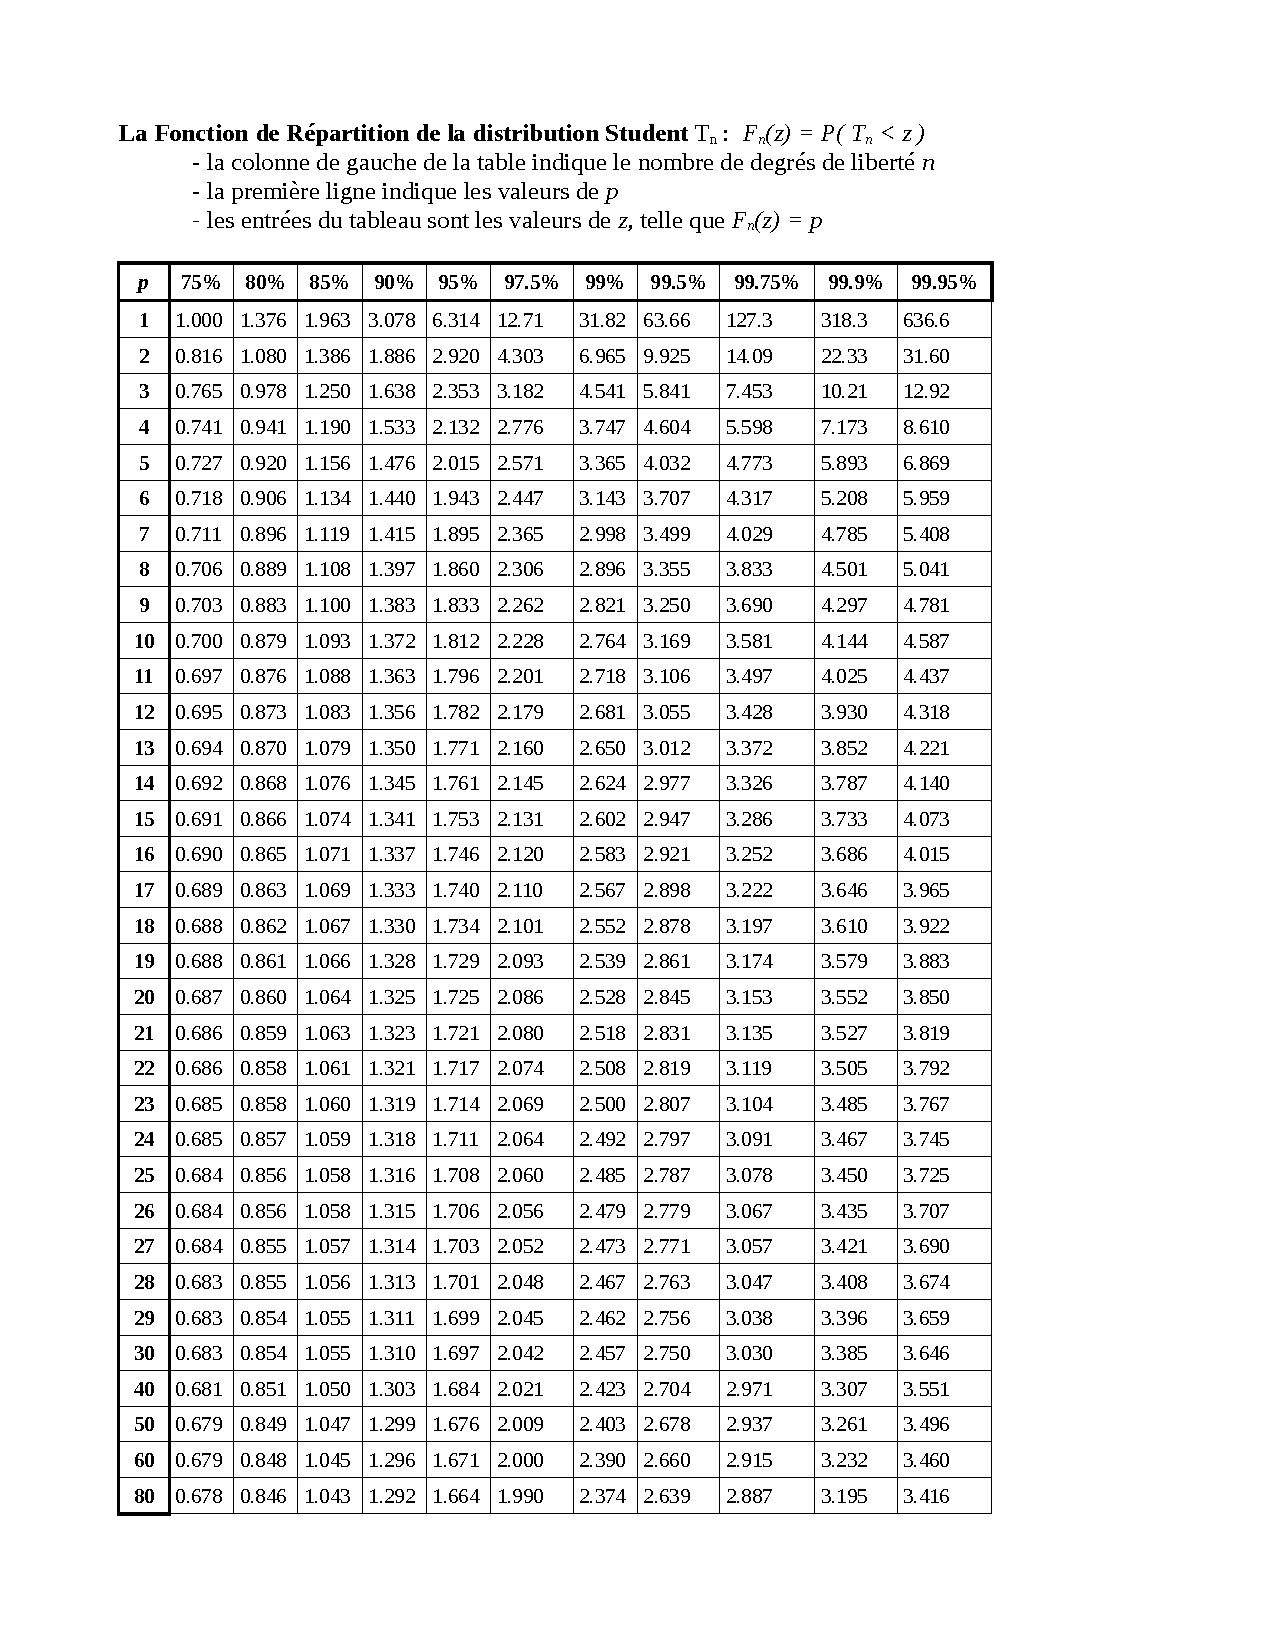
\includepdf{table1.pdf}
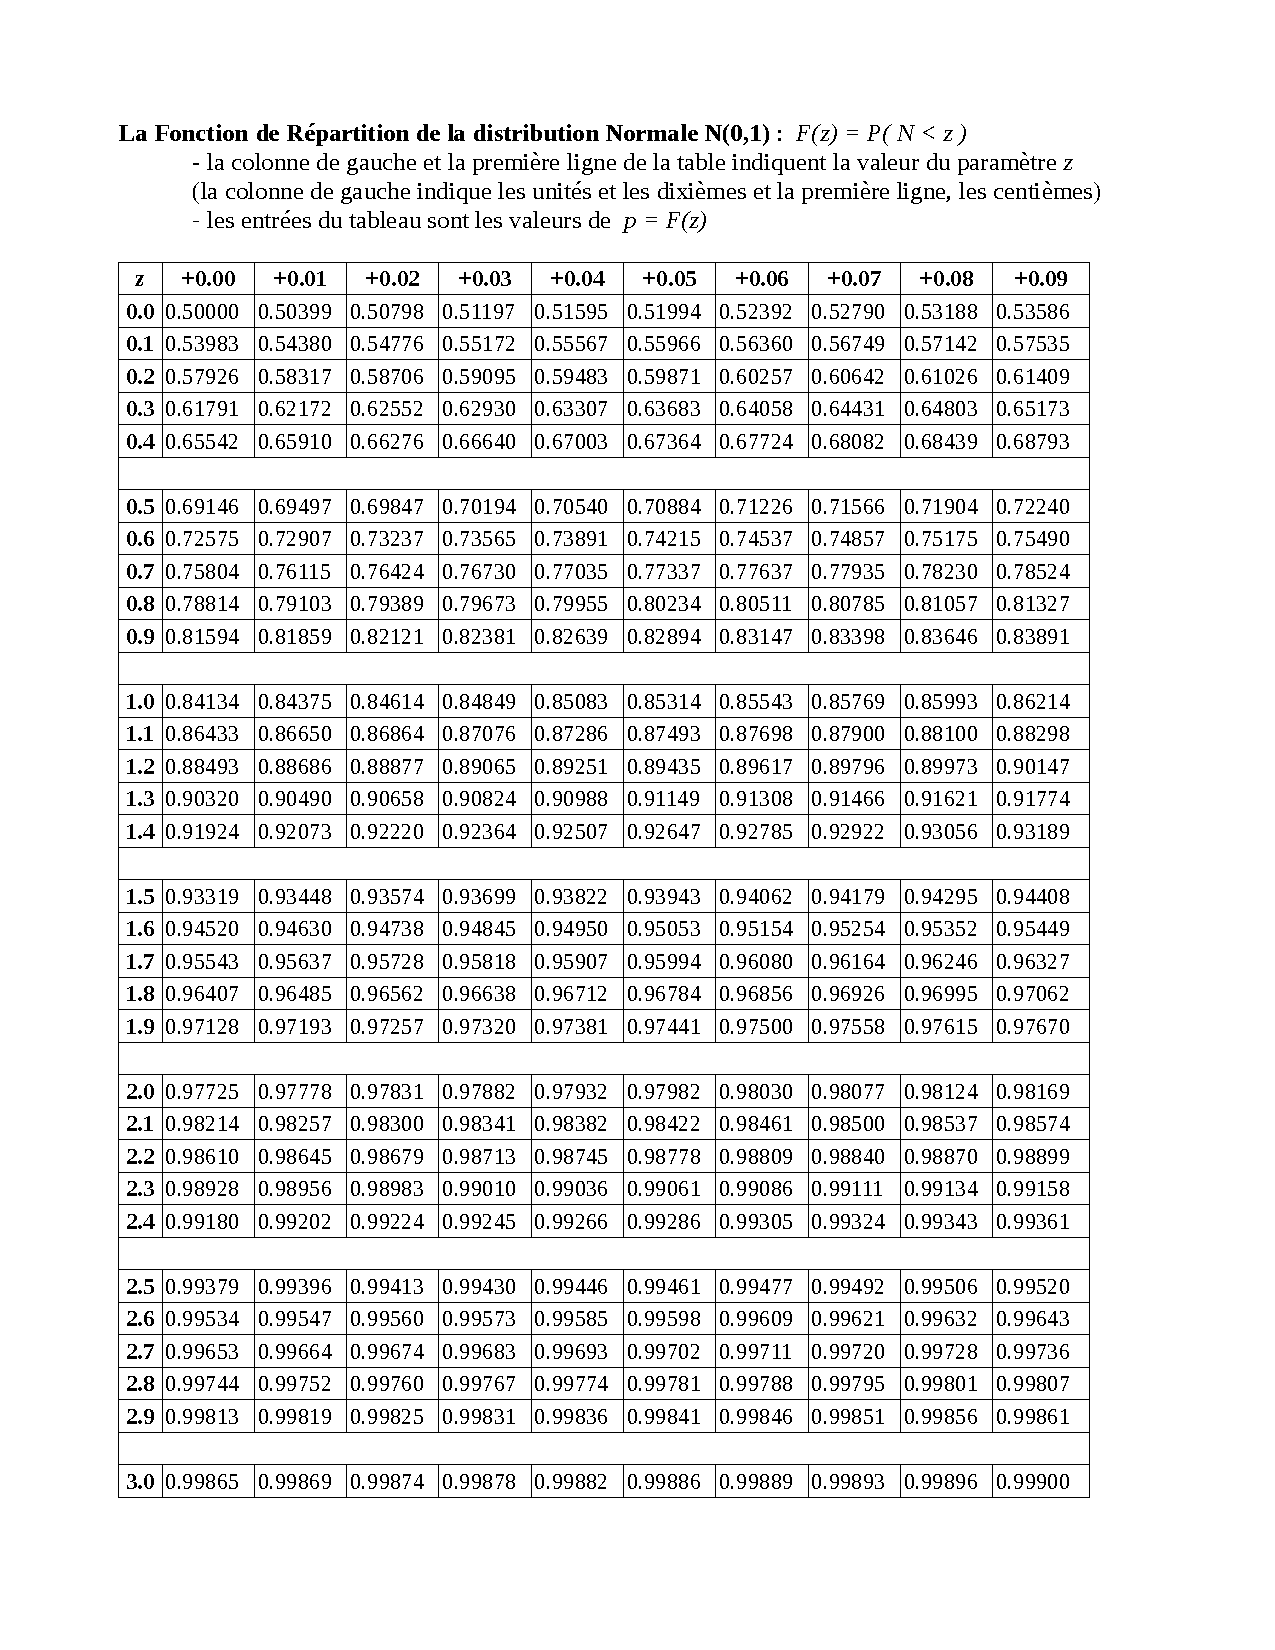
\includepdf{table2.pdf}

\end{document}

















    \begin{exmp}
        Si on considère le lancé d'un pièce, alors $\Omega = \{ pile,face\}$ auquel cas $\#\Omega = 2$.\\
        Si le résultat qu'on observe est la face qui apparaît après le lancé d'un dé non-pipé\footnote{c'est-à-dire dont chaque face est équiprobable}, alors $\Omega = \{1,2,3,4,5,6\}$ auquel cas $\#\Omega = 6$.
    \end{exmp}
    
    \begin{exmp}
        Prenons un jeu de $52$ cartes qu'on distribue à tout les joueurs. S'il y a quatre joueurs, quelle est la probabilité de $A =$"chaque joueur a un as" ? D'après ce qu'on a vu plus haut, $|A| = 4!\frac{48!}{(12!)^4}$ parce qu'on peut commencer par donner un as à chaque joueur ($4!$) puis on distribue les $48$ cartes restantes et $|\Omega| = \frac{52!}{(13!)^4}$, donc $$\P(A) = \frac{|A|}{|\Omega|} = 0,105$$
    \end{exmp}

    \begin{exmp}
        Soit le lancé de deux dés non-pipés, $\Omega = \{(1,1),(1,2),\dots,(6,6) \}$. On considère l'évènement $A=$ "la somme des résultats est égale à 5". Dans ce cas $A = \{ (1,4),(4,1),(2,3),(3,2)\}$. On peut donc dire que si on lance deux dés, la probabilité que les somme des résultats est égale à 5 est
        $$\P(A) = \frac{\#A}{\#\Omega} = \frac{4}{36} = \frac{1}{9}$$
    \end{exmp}
    
    Dans un système de cause ($A$) à effet ($B$) du type $A\Ra B$, il souvent utile de connaître la lien dans le sens inverse $B\Ra A$, c'est-à-dire de connaître $\P(A|B)$. On appel ça un \d{problème d'inférence}. En utilisant la troisième loi et développant quelques termes, nous pouvons exprimer $\P(A |B)$ en fonction de $\P(B|A)$ et de d'autres probabilités faciles à obtenir. La forme est la suivante :
        \begin{center}
            \fbox{$\displaystyle{\P(A|B) = \frac{\P(A)\P(B|A)}{\P(A)\P(B|A)+\P(\bar{A})\P(B|\bar{A})}}$}
        \end{center}

        \begin{leftbar}
            \begin{defn}
                Deux évènements $A$ et $B$ sont dis \d{indépendants} si et seulement la probabilité de l'un est indépendante du fait que l'autre se soit produit ou pas. C'est-à-dire que 
                $$\P(AB) = \P(A)\P(B) \Leftrightarrow \P(A|B) = \P(A) \text{ et } \P(B|A) = \P(B)$$
            \end{defn}
        \end{leftbar}
        
    \begin{exmp}
        On veut trouver $n$ telle que la probabilité de $A =$"au moins 2 personnes ont leur anniversaire le même jour" soit $\P(a)>\frac{1}{2}$. On sait que $n\leq365$ car si $n\geq 365$, $\P(A) = 1$. Nous avons que $\#\Omega = 365^n$. De plus, $\bar{A} =$ "personne n'a son anniversaire le même jour" et par conséquent $\#\bar{A} = A_{365}^n = \frac{365!}{(n-365)!}$. Pour trouver $\#A$ il ne reste plus qu'à utiliser la relation $\#A = \#\Omega-\#\bar{A}$. D'où $$\P(A) = \frac{\#A}{\#\Omega} = \frac{\#\Omega-\#\bar{A}}{\#\Omega} = 1-\frac{365!}{(n-365)!365^n}$$
        La solution peut alors être trouvée graphiquement. On obtient $n\approx 23$.
    \end{exmp}
    
    \begin{exmp}
        Imaginons $n$ antennes téléphoniques dont $m < n$ sont défectueuses. La transmission est assurée si aucunes antennes défectueuses sont voisines. Prenons $A=$ "transmission assurée". Dans ce cas $|A| = {n-m+1\choose m}$ parce qu'on peut commencer par placer les $n-m$ antennes qui fonctionnent bien et il reste alors $n-m+1$ possibilité (extrémités + entre deux antennes déjà placées) pour placer les $m$ antennes restantes. Et $|\Omega| = {n\choose m}$. Cela implique que 
        $$\P(A) = \frac{|A|}{|\Omega|} = \frac{{n-m+1\choose m}}{ {n\choose m}}$$
    \end{exmp}
    
    \subsection{Probabilité Bayesienne}
    
    
        \begin{leftbar}
        \begin{defn} La \d{probabilité Bayesienne} d'une proposition est un nombre qui quantifie la vraisemblance de cette proposition conditionnée à un certain état d'information sur cette proposition :
            $$\P(A,I) \neq \P(A,I')$$
        où $\P(A,I)$ est la probabilité de $A$ compte tenu d'une information $I$.
        \end{defn}
        \end{leftbar}
        
            \subsection{$X$ continue et $Y$ discrète}
        
            De nouveau en combinant les deux premiers cas, nous obtenons
            $$f_{X|Y=y}(x) = \frac{f_X(x)\P_{Y|X=x}(y)}{\P_Y(y)} = \frac{f_X(x)\P_{Y|X=x}(y)}{\int_{-\infty}^{+\infty}f_X(x)~dx~\P_{Y|X=x}(y)}$$

%schémas  : système avec les billes, chauqe distribution usuelle,arbre principe multiplicatif
%sch 3d distrib conjointe continue
%sch 3d distrib conjoite discrète